\documentclass[
        oneside,      %%coloque  % no in\'icio desta linha para imprimir frente e verso 
        english,			
%	french,				
%	spanish, 
        brazil			 
        ]{abntbibufjf}


\usepackage[T1]{fontenc}		
\usepackage[utf8]{inputenc}		%% Para converter automaticamente acentos como digitados normalmente no teclado. Mude utf8 para latin1 se precisar. 

\usepackage{lmodern} %no caso do modelo Latex, pode-se usar a fam\'ilia de fontes lmodern como aqui indicado, no lugar de Arial e Times New Roman.

\usepackage{amsmath} % Pacote para melhorar a formatação de equações
\usepackage{lastpage}
\usepackage{indentfirst}
\usepackage{color}
\usepackage{graphicx}
\usepackage{microtype}
\usepackage{hyperref}
\usepackage{xurl}
\usepackage{xcolor}
\usepackage{fancyvrb}
% \usepackage[table]{xcolor}
\usepackage{makecell}
\usepackage{todonotes}
\usepackage{chngcntr}
\usepackage{multirow}

\counterwithin{figure}{chapter}
\counterwithin{table}{chapter}

\bibliographystyle{plainnat}

%% -----------------------------------------------------------------------------

%% Obs.: Alguns acentos foram omitidos.

\titulo{Aprendizado de máquina com dados categóricos na modelagem chuva-vazão para previsão de vazão em bacias hidrográficas de Minas Gerais} %% Colocar, dentro de chaves {}, o t\'itulo do trabalho. 
%\subtitulo{subt\'itulo}  %% Colocar % no in\'icio desta linha se nao tiver subt\'itulo 
\autor{Welson de Avelar Soares Filho} %%Colocar, dentro de chaves {}, o nome completo do autor
\autorVirg{Soares Filho, Welson de Avelar} %%Colocar o sobrenome do autor, separado por v\'rgula, antes do restante do nome do autor. Ex.: Santos, Maria dos
\local{Juiz de Fora} %%Governador Valadares % N\~ao usar MG.
\data{2024} %%Colocar o ano da entrega. Por exemplo, 2019. N\~ao usar m\^es.
\orientador[Orientador:]{Leonardo Goliatt} %%Se precisar, troque [Orientador:] por [Orientadora:]
%\coorientador[Coorientador:]{Nome e sobrenome} %% Colocar ``%'' no in\'icio desta linha se n\~ao tiver coorientador. Se precisar, troque por [Cooorientadora:]. 
\orientadorTitulo{Doutor} %%Colocar, dentro de chaves {}, a titula\c{c}\~ao do(a) orientador(a). Por exemplo, Prof. Dr.
%\coorientadorTitulo{Doutora} %%Colocar, dentro de chaves {}, a titula\c{c}\~ao do(a) cooorientador(a). 
\instituicao{Universidade Federal de Juiz de Fora}
\faculdade{Instituto de Ciências Exatas} %%Colocar, dentro de chaves {}, o nome da faculdade ou do instituto.
\programa{Programa de Pós-Graduação em Modelagem Computacional} %%Colocar, dentro de chaves {}, o nome do curso. Por exemplo: Programa de P\'os\mbox{-Gra}dua\c{c}\~ao em Matem\'atica
\objeto{Dissertação (Mestrado)}  %%Tese (Doutorado)  %%%Trabalho de Conclus\~ao de Curso (gradua\c{c}\~ao)
\natureza{Dissertação  %%Tese 
apresentada ao \insereprograma ~da   %% %%%Trabalho de conclus\~ao de curso apresentado \'a \inserefaculdade da %%%%SUBSTITUIR \'a POR ao SE FOR INSTITUTO    
Universidade Federal de Juiz de Fora como requisito parcial \`a obten\c{c}\~ao do 
t\'itulo de Mestre em  %%Doutor em    %%%grau de bacharel em 
Modelagem Computacional. %%Trocar Matem\'atica por outro, se precisar.
\'Area de concentra\c{c}\~ao: Modelagem Computacional%%PREENCHER   %%%N\~ao usar esta linha se for trabalho de conclus\~ao de curso da gradua\c{c}\~ao
}

%% Abaixo, prencher com os dados da parte final da ficha catalografica
\finalcatalog{1. recursos hídricos. 2. redes neurais. 3. previsão de vazão. I. Goliatt, Leonardo, orient. II. Doutor.} %% Aqui fica 
% escrito a palavra ``T\'itulo'' mesmo, nao o do trabalho. Se tiver coorientador, os dados ficam depois dos dados 
%% do orientador (II. Sobrenome, Nome do coorientador, coorient.) e antes de ``II. T\'itulo'', o qual passa a ``III. T\'itulo''.


\usepackage[round, numbers]{natbib} %para refer\^encias bibliogr\'aficas no sistema num\'erico com () na chamada da citacao. 

%Se for usar o sistema autor-data, colocar % antes de \usepackage acima e retirar % antes de \usepackage abaixo.

%\usepackage{natbib} %para o sistema autor-data

\begin{document}

\renewcommand{\labelitemi}{$\bullet$}  % Marcador de itens no nível 1
\renewcommand{\labelitemii}{$\diamond$}

%% ELEMENTOS PR\'E-TEXTUAIS

%% Capa. N\~ao entra na contagem da pagina\c{c}\~ao.
\inserecapa

%% Folha de rosto
\inserefolhaderosto

%% Ficha catalogr\'afica. AO IMPRIMIR, DEIXAR NO VERSO DA FOLHA DE ROSTO.
\inserecatalog  


%% Folha de aprovacao. Incluir mesmo que sem assinaturas. Assinaturas eletr\^onicas via SEI.
\begin{folhadeaprovacao}
\inicfolhaaprov
        
Aprovada em (dia) de (m\^es) de (ano) %%Preencher com a data 
   
\vfill
\begin{center} BANCA EXAMINADORA \end{center}
\assinatura{\insereorientadorTitulo~\insereorientador \ - Orientador \\ Universidade Federal de Juiz de Fora}  %%Orientadora
%\assinatura{Professor Dr. \inserecoorientador \ - Coorientador \\ Universidade Federal de Juiz de Fora}
\assinatura{Titula\c{c}\~ao Nome e sobrenome \\ Universidade ???}
\assinatura{Titula\c{c}\~ao Nome e sobrenome  \\ Universidade ??} 
%\assinatura{...} %%RETIRE O % E PREENCHA SE PRECISAR
%  \assinatura{...}
%  \assinatura{...}
\end{folhadeaprovacao}
\cleardoublepage 


%% Dedicatoria. OPCIONAL. N\~ao deve haver t\'itulo. Colocar ``%'' no in\'icio de cada das 3 linhas abaixo, caso n\~ao queira. 
 \begin{dedicatoria} 
  %Dedico este trabalho ... 
 \end{dedicatoria}
 
%% Agradecimentos. OPCIONAL. Caso seja bolsista, inserir os devidos agradecimentos.
\begin{agradecimentos}
Agradeço aos meus pais, Regina e Welson, por terem se dedicado, desde sempre, para que eu, meu irmão e irmã, buscássemos nos aprimorar enquanto cidadãos através dos estudos. A participação e acompanhamento em cima de nossos estudos fixaram em mim o desejo pela busca do conhecimento. Este trabalho tem parte de vocês. Muito obrigado.

Meu irmão Raphael e irmã Patrícia. Precisei me abster, em muito, de seu convívio, mas eu nunca esqueci de seu companheirismo, de sua amizade e do quanto apoio tive neste momento da vida.

Minha noiva, Juliana, minha companheira, que tanto precisou abdicar de seu próprio lazer, de feriados e finais de semana, para que eu ficasse em casa totalmente dedicado e focado neste trabalho. Obrigado por tanto e a vida ao seu lado é, certamente, mais saborosa por isso.

Ao Instituto Federal de Educação, Ciência e Tecnologia do Sudeste de Minas Gerais, em especial ao campus de Juiz de Fora, por ter me apoiado no meu desejo de qualificar através do mestrado. Eu saí um tipo de servidor público e retorno agora bastante diferente, e desejo, profundamente, contribuir com a instituição e comunidade acadêmica para nosso aprimoramento.

Todos amigos de repartição, que aqui faço questão de nomear: Diego, Matheus, Bruno, Marcus e Jacqueline. Precisaram cobrir minhas atividades, e o fizeram com maestria, enquanto eu me dedicava ao mestrado. Vocês moram em meu coração.

Meus amigos e amigas pessoais que pouco me viram neste período, familiares também. Jamais esqueci de vocês e o quanto torciam por mim e pelo meu sucesso no cumprimento da atividade enquanto estive ausente do nosso viver. Tivemos conversas apenas por aplicativos, distantes, e anseio poder rever seus olhos.

Aos meus colegas do PGMC: meu muito obrigado. Conhecer pessoas tão incríveis com certeza ajuda a compor a relevância deste trabalho, e a amizade de vocês tornou a caminhada menos árdua.

Leonardo, meu caro orientador. Obrigado por partilhar de seu conhecimento comigo. Suas dicas e observações irão comigo onde quer que eu vá, onde quer que eu esteja.

Ao professor Celso Bandeira e à colega de projeto Paula pelas conversas e debates sobre os trabalhos desenvolvidos, ideias e tudo mais.

E, finalmente, à Rhama Analysis pela gentileza em me conceder acesso ao seu principal sistema de dados hidrológicos quando mais precisei e à Agência Nacional de Águas e Saneamento Básico (ANA) pelo hercúleo trabalho desenvolvido na gestão e conhecimento de nossas águas.

Meu muito obrigado.
\end{agradecimentos}


%% Ep\'igrafe. OPCIONAL. Com os dados do autor. A obra usada na ep\'igrafe deve constar nas refer\^encias. 

% Quando at\'e 3 linhas: \'e obrigat\'orio o uso de aspas duplas.

%\begin{epigrafemenos} %%Ep\'igrafe com 3 ou menos linhas
%``Mas para que o produto de uma pesquisa científica possa ser publicado não basta que ele apresente um conteúdo de qualidade, também é exigida qualidade de forma.'' (MAR\c{C}AL JUNIOR, 2013, p. 19-20).
%\end{epigrafemenos}

%%Quando com mais de 3 linhas.
\begin{epigrafemais} %%Ep\'igrafe com mais de 3 linhas 
	% Elemento opcional, em que o autor apresenta uma cita\c{c}\~ao, seguida de indica\c{c}\~ao de autoria, relacionada com a                       
 %  mat\'eria tratada no corpo do trabalho. (ASSOCIA\c{C}\~AO BRASILEIRA DE NORMAS T\'ECNICAS, 2011, p. 2).
\end{epigrafemais}


%% RESUMOS

%% Resumo em Portugu\^es. OBRIGAT\'ORIO. \'E obrigat\'orio o uso de par\'agrafo \'unico.
\begin{resumo}

Resumo do trabalho \\[18pt]
Palavras-chave: Aprendizado de máquina. Recursos hídricos. Previsão de vazão. %Finalizadas por ponto e inicializadas por letra maiuscula.
\end{resumo}
 
 
%% Resumo em Ingl\^es. \'E obrigat\'orio o uso de par\'agrafo \'unico.
\begin{resumo}[ABSTRACT]
 \begin{otherlanguage*}{english}

Project summary \\[18pt]
Keywords: Machine learning. Water resources. Runoff forecasting. %Finalizadas por ponto e inicializadas por letra maiuscula.
 \end{otherlanguage*}
\end{resumo}

%% Seguindo o mesmo modelo acima, pode-se inserir resumos em outras l\'inguas. 



%% Lista de ilustra\c{c}\~oes. OPCIONAL. Sao consideradas ilustra\c{c}\~oes: desenhos, esquemas, fluxogramas, figuras, fotografias, gr\'aficos, mapas, organogramas, plantas, quadros, entre outros. Tabelas n\~ao s\~ao consideradas ilustra\c{c}\~oes. A ordem da lista deve obrigatoriamente ser a mesma ordem em que as ilustra\c{c}\~oes aparecem no texto. Quando o t\'itulo ocupar mais de uma linha, a segunda linha deve estar exatamente abaixo da primeira.  

\pdfbookmark[0]{\listfigurename}{lof}

%Caso as ilustra\c{c}~oes do trabalho sejam todas do mesmo tipo (por exemplo, todas do tipo organograma), coloque % no in\'icio das duas linhas abaixo. 
\ilustvaria   %Use este comando somente caso as ilustra\c{c}\~oes n\~ao sejam todas do mesmo tipo. 
\listilustvaria  %Use este comando somente caso as ilustra\c{c}\~oes n\~ao sejam todas do mesmo tipo e caso queira inserir a lista delas. 

%\listoffigures*  %Use este comando quando todas as ilustra\c{c}\~oes s\~ao do mesmo tipo e caso queira inserir a lista delas. Veja dicas no final deste arquivo.

\cleardoublepage
\pdfbookmark[0]{\listtablename}{lot}

%% Lista de tabelas. OPCIONAL. A ordem da lista de tabelas deve obrigatoriamente ser a mesma ordem em que as tabelas aparecem no texto. 


\listoftables*    %Coloque ``%'' no in\'icio desta linha, caso n\~ao queira lista de tabelas. 

\cleardoublepage


%% Lista de abreviaturas e siglas. OPCIONAL. Nao deve haver sinal grafico entre as siglas e abreviaturas e o significado. 

\begin{siglas} %%ALTERAR OS EXEMPLOS ABAIXO, CONFORME A NECESSIDADE
  \item[ANA] Agência Nacional de Águas e Saneamento Básico
  \item[Fil.] Filosofia 
  \item[IBGE] Instituto Brasileiro de Geografia e Estat\'istica 
  \item[INMETRO] Instituto Nacional de Metrologia, Normaliza\c{c}\~ao e Qualidade Industrial
  \end{siglas}

%% Lista de s\'imbolos. OPCIONAL. Nao deve haver sinal grafico entre o simbolo e o seu significado.

\begin{simbolos} %%ALTERAR OS EXEMPLOS ABAIXO, CONFORME A NECESSIDADE
  \item[$ \forall $] Para todo
  \item[$ \in $] Pertence
 \end{simbolos}

 
%% Sum\'ario

\pdfbookmark[0]{\contentsname}{toc}
\tableofcontents*
\cleardoublepage

%% ----------------------------------------------------------

%% ELEMENTOS TEXTUAIS
\textual

\chapter{INTRODU\c{C}\~AO}  %%Nesta linha, dentro de { }, digita-se em CAIXA ALTA, como apresentado aqui

% \begin{itemize}
	%     \item \textbf{use o comando cite para fazer a citação so com o número da referencia \cite{rayyan-33388112}}
	
	%     \item \textbf{use o comando citet para fazer a citação com o nome do autor e o numero da referencia \citet{rayyan-33388114}}
	% \end{itemize}

% \begin{figure}[htb!]
	%     \centering
	%     
\includegraphics[width=0.5\linewidth]{Figuras/google.png}
	%     \caption{Caption}
	%     \label{fig:enter-label}
	% \end{figure}

% \begin{figure}[htb!]
	%     \centering
	%     
\includegraphics[scale=0.3]{Figuras/google.png}
	%     \caption{Caption}
	%     \label{fig:enter-label}
	% \end{figure}

A gestão dos recursos hídricos desempenha um papel crucial nas políticas públicas. Nos âmbitos socioeconômico, cultural e de saúde pública, conhecer a dinâmica dos recursos hídricos e entender como fatores externos impactam seu comportamento é de grande importância para os administradores públicos. A compreensão desses aspectos permite uma melhor tomada de decisões, garantindo a sustentabilidade dos recursos, a segurança hídrica e o bem-estar da população.

Neste sentido, prever a vazão de rios é um componente essencial na gestão de recursos hídricos, operação de reservatórios e mitigação de desastres naturais, especialmente em regiões onde a hidroelectricidade desempenha um papel crucial na matriz energética, como é o caso do Brasil\todo[color=blue,textcolor=white]{tem referencia para esta parte? seria bom colocar alguma coisa}. De acordo com o Balanço Energético Nacional de 2023, ano-base 2022, divulgado pelo Ministério de Minas e Energia, esta matriz energética representa cerca de 64\% da oferta interna total de geração de energia elétrica \cite{epe2023ben}. Desta forma, a previsão da vazão dos rios que abastecem os reservatórios das hidrelétricas tem importância no impacto econômico que uma usina em baixa capacidade de geração pode causar.

Em uma perspectiva mais direcionada à população, os rios abastecem represas e açudes que fornecem água potável para consumo humano e animal, além de irrigar a lavoura \todo[color=blue, textcolor=white]{referencia?}. Não apenas os rios, mas também a chuva têm impacto significativo nesse cenário. Uma análise criteriosa da previsibilidade da vazão dos rios nos dias seguintes permite ao poder público, por exemplo, reduzir ou até mesmo suspender outorgas para retirada de água, visando o bem-estar populacional. Além disso, essa análise pode auxiliar no planejamento de regimes de racionamento. Basta lembrarmos do ano de 2015, quando noticiava-se o 'uso do volume morto' \todo[color=blue, textcolor=white]{aspas no latex é feito assim ''exemplo de aspas'', deixe as aspas simples para as variáveis utilizadas nos eu modelo} na Cantareira, no estado de São Paulo, pois a estiagem fora além do previsto e o abastecimento de cidades, da cidade de São Paulo propriamente, foram severamente afetados.\cite{g1_cantareira_2015}

E quando se fala em bem-estar populacional, não podemos deixar de considerar os eventos climáticos extremos. 

%No Brasil, a ocorrência de inundações em áreas urbanas tem-se intensificado devido a diversos fatores, dentre eles a urbanização acelerada e a ocupação inadequada do solo. Além da impermeabilização dos solos, falta infraestrutura nos municípios e o desmatamento ciliar também contribui para as inundações, favorecendo o aumento do volume de vazão e a velocidade de propagação da onda de inundação em regiões onde os eventos hidrológicos constituem um risco de desastre natural (ref. CEMADEN).

Basta lembrar dos últimos desastres ocorridos nos estados de Minas Gerais, Rio de Janeiro, Paraná, São Paulo e Bahia que trouxeram não só perda econômica como também perda de vidas humanas. \cite{bbc_chuvas_bahia_2024} \cite{cnn_temporais_mg_2024} \cite{g1_temporal_es_2024} \cite{g1_temporal_petropolis_2022}

Especificamente no estado de Minas Gerais há lacunas de conhecimento sobre os processos hidrológicos das bacias hidrográficas

\section{Contextualização}
%Introduzir o tema, contextualizando a área de estudo e a relevância da pesquisa.

\section{Justificativa}
%Explicar porque a pesquisa é importante e quais são contribuições.

\section{Problema de pesquisa}
%Definir claramente o problema que a pesquisa busca resolver.

\section{Objetivos}

\todo[inline, color=blue, textcolor=white]{Separa objetivo e objetivo específico em seções}
O trabalho tem como escopo a modelagem de recursos hídricos baseada em dados históricos de vazão, contrastando com os modelos físicos tradicionalmente aplicados na área, como o modelo SMAP (Soil Moisture Accounting Procedure) e o SWAT (Soil and Water Assessment Tool). Ao invés de utilizar as abordagens físicas que simulam processos hidrológicos baseados em equações diferenciais e características fisiográficas das bacias, a proposta é aplicar métodos de modelagem orientados a dados para prever séries temporais univariadas de vazão. Essas previsões serão realizadas com o suporte de variáveis exógenas, como precipitação, e variáveis categóricas, a serem melhor descritas a posteri, que ajudam a capturar a sazonalidade e outros padrões importantes do regime de águas.

\todo[inline, color=blue, textcolor=white]{O objetivo específico deve vir em tópicos e em uma subseção do objetivo}
O objetivo mais específico é desenvolver um modelo de previsão eficiente e preciso que possa ser utilizado para auxiliar na gestão dos recursos hídricos em Minas Gerais. Em uma etapa posterior, pretende-se criar uma aplicação web para disponibilizar essas previsões ao Instituto Mineiro de Gestão das Águas (IGAM \cite{igam_site_2024}), permitindo que as informações estejam acessíveis para planejamento e tomada de decisões estratégicas.

Este trabalho se insere como um componente fundamental de um sistema gerencial maior, que visa aprimorar o planejamento e a gestão dos recursos hídricos do estado de Minas Gerais. Ao integrar previsões baseadas em dados históricos, o modelo permitirá uma melhor alocação dos recursos, suporte em períodos críticos, como secas e enchentes, e uma gestão mais eficiente das bacias hidrográficas do estado. \todo[color=blue,textcolor=white]{esta parte me parece mais uma descrição do trabalho do que um objetivo propriamente dito}

\section{Estrutura da Dissertação}
\todo[inline, color=blue, textcolor=white]{não é muito usual, alguns membros da banca podem não gostar, verificar com o léo se cabe esta parte na sua dissertação}
Resumo breve da organização dos capítulos.
\chapter{REVIS\~AO DA LITERATURA SOBRE O TEMA}
\section{Conceitos Teóricos Fundamentais}
Conceitos e teorias básicas relacionadas ao tema.

\section{Estudos Relacionados}
Revisar literatura existente, destacar pesquisas similares e identificar lacunas.

\section{Aprendizado de Máquina na Hidrologia}
Discutir a aplicação de técnicas de ML na hidrologia, citando estudos relevantes.

\section{Dados de Precipitação e Vazão}
Descrever os tipos de dados utilizados no estudo e respectivas fontes.

\section{Modelos de Previsão de Vazão}
Comparar diferentes modelos de previsão de vazão (vou comparar com SeasonalNaive e Linear Regression, duas baselines comumente aplicadas).
\chapter{PROCEDIMENTOS METODOLÓGICOS}
\section{Descrição da Área de Estudo}
%Detalhar a localização e características da minha área de estudo.

\todo[inline]{FAZER IMAGEM DAS BACIAS}

As bacias de estudo são as bacias dos rios Jequitinhonha, Doce, Grande e São Francisco. Em todas estas, o corpo d'água principal da bacia, seus respectivos rios, passam dentro do estado de Minas Gerais, por isso a escolha. Isso é para distinguir do não uso do rio Paraíba do Sul no estudo, visto que parte de sua bacia está nos limites do estado, mas o rio não passa dentro dos limites administrativos estaduais.

O rio Jequitinhonha, com sua bacia hidrográfica abrangendo cerca de 65 mil quilômetros quadrados, é uma peça fundamental na paisagem e na vida socioeconômica de Minas Gerais. Seu curso percorre 82 municípios mineiros, abrigando uma população de aproximadamente 939 mil habitantes que dependem diretamente de suas águas.\cite{ibge} \cite{jequiti_igam_mg_1} \cite{jequiti_igam_mg_2} \cite{jequiti_igam_mg_3}

A Mata Atlântica é o bioma predominante e a atividade econômica principal na região é a agropecuária, ocupando uma área considerável de 2,6 milhões de hectares, em contraste com os 3,8 milhões de hectares de floresta. Essa dinâmica evidencia a pressão exercida sobre o ecossistema, demandando um olhar atento para a gestão sustentável dos recursos naturais.\cite{mapbiomas}

O rio Doce, com sua nascente na Serra da Mantiqueira, em Minas Gerais, percorre 853 quilômetros até desaguar no Oceano Atlântico, no Espírito Santo, delineando uma bacia hidrográfica muito importante para o Sudeste brasileiro. Com uma área de drenagem de 86 mil quilômetros quadrados, abriga 200 municípios mineiros, onde residem cerca de 3,5 milhões de pessoas, e desempenha um papel crucial na dinâmica socioeconômica e ambiental da região. 

A predominância da Mata Atlântica, com uma pequena fração de Cerrado, confere à bacia uma vasta biodiversidade, ao mesmo tempo em que a coloca em posição de vulnerabilidade frente às pressões antrópicas. As principais atividades ecônomicas são a agropecuária, a agroindústria e o setor de mineração/siderurgia (Quadrilátero Ferrífero) e impulsionam a economia regional. A cobertura do solo, com 2,4 milhões de hectares de floresta e 5,5 milhões de hectares dedicados à agropecuária, reflete essa dualidade entre desenvolvimento e preservação.

O rio Grande é um dos cursos d'água mais importantes do Brasil, escorrendo por Minas Gerais e São Paulo até se unir ao rio Paranaíba e formar o rio Paraná. Com uma área de drenagem de 143 mil quilômetros quadrados, sua bacia abrange 393 municípios, impactando a vida de cerca de 9 milhões de pessoas. 

Nascido na Serra da Mantiqueira, o rio Grande é um rio de planalto, percorrendo 1286 km até seu encontro com o Paranaíba. O Cerrado é o bioma predominante em sua bacia, com trechos que se limitam à Mata Atlântica, criando uma rica diversidade de ecossistemas.

A agroindústria é a principal atividade econômica na região, impulsionada pela fertilidade do solo e pela disponibilidade de água. No entanto, o rio Grande também é fundamental para a geração de energia elétrica, abrigando 13 barragens, incluindo a importante usina de Furnas. Essa combinação de agropecuária e geração de energia molda a paisagem da bacia, com 11,1 milhões de hectares dedicados à agricultura e 2,1 milhões de hectares cobertos por florestas.

Por fim, mas certamente, não menos importante, rio São Francisco. Carinhosamente apelidado de ``Velho Chico'', conecta regiões, culturas e economias ao longo de seus quase 3 mil quilômetros de extensão. Com uma bacia hidrográfica que abrange 639 mil quilômetros quadrados, a bacia do São Francisco corresponde a 8\% do território nacional, impactando diretamente a vida de cerca de 15 milhões de pessoas.

Sua grandiosidade é tamanha que sua bacia abrange seis estados brasileiros - Minas Gerais, Goiás, Bahia, Pernambuco, Alagoas e Sergipe - e devido à tanta complexidade, a bacia é dividida em quatro regiões fisiográficas distintas: Alto, Médio, Submédio e Baixo São Francisco, cada qual com particularidades geográficas, sociais e econômicas.

A diversidade de biomas que o Velho Chico atravessa é outro ponto marcante: do Cerrado à Caatinga, passando por fragmentos da Mata Atlântica, essa variedade se reflete também na cobertura do solo de sua bacia, com predominância de áreas destinadas à agropecuária (12,4 milhões de hectares) e florestas (15,3 milhões de hectares), indicando a importância tanto da produção agrícola quanto da preservação ambiental. Suas águas impulsionam atividades como a siderurgia, mineração, indústria química e têxtil, além de pesca e agropecuária.

%O rio São Francisco é também um fenômeno cultural. Diversos poetas, cantores e escritores já escreveram sobre suas águas. Estudá-lo e compreendê-lo é também ajudar a manter viva sua poesia.

\section{Dados Utilizados}
\todo[inline]{FAZER IMAGEM DE ONDE ESTÃO AS ESTAÇÕES}

A coleta dos dados foi realizada com um misto da biblioteca HydroBR \cite{carvalho2020hydrobr} e funções próprias de extração de dados. A biblioteca permitiu a listagem de todas as estações hidrométricas disponíveis, como, por exemplo, as estações convencionais de medição de vazão. Após a identificação e seleção das estações de interesse, cujos códigos estavam disponíveis na base de dados da ANA, desenvolveu-se um conjunto de funções para automatizar o processo de extração. Essas funções permitiram o \textit{download} dos dados referentes ao período especificado diretamente do \textit{webservice} fornecido pela ANA.

O período de dados analisado compreende \textbf{de 1º de janeiro de 2013 a 31 de dezembro de 2023}, totalizando 11 anos completos.

Foram utilizadas \textbf{séries temporais diárias} de precipitação e vazão. As colunas correspondentes às datas foram formatadas como ``\textit{datetime}'', enquanto os dados de precipitação e vazão foram representados como valores de ponto flutuante (``\textit{float}''). Embora a frequência diária tenha sido adotada, é importante destacar que nem todas as séries temporais estavam originalmente nesse formato. Foi necessário lidar com quebra na continuidade das datas e com dados ausentes. Estes aspectos serão discutidos em detalhes em seções subsequentes.

Os dados de precipitação e vazão obtidos do site da ANA já estavam ajustados nas escalas padrão utilizadas em estudos hidrológicos. A precipitação foi fornecida em milímetros por dia (mm/dia), refletindo a quantidade de chuva que cai sobre uma unidade de área em um período de 24 horas e as vazões, por sua vez, foram disponibilizadas em metros cúbicos por segundo (m³/s), indicando o volume de água que passa por uma seção transversal do rio a cada segundo. Em algumas estações, foram observados valores extremamente elevados para determinados dias, tanto nas séries de precipitação quanto nas de vazão, os quais podem ser considerados \textit{outliers}. Em relação aos dados de vazão, verificou-se a ocorrência de valores nulos (vazão igual a 0), o que indicaria a interrupção completa do fluxo do rio. Esse fenômeno, no entanto, não faz sentido, considerando que não há registro de eventos de seca tão severos nos rios analisados. Apesar destas anomalias, os dados não foram descartados, pois tanto os registros de vazão quanto os de precipitação utilizados nesta pesquisa foram considerados consistidos pela ANA, ou seja, foram medidos e validados pela agência. O presente trabalho não questionou a veracidade dos dados; eles foram utilizados conforme disponibilizados pela ANA.

É relevante destacar que a consulta prévia ao sistema \textit{on-line} da ANA foi essencial, pois frequentemente selecionavam-se códigos de estação que, ao final, não possuíam dados para o período especificado ou apresentavam códigos alterados na base de dados, sendo retornados como ``inexistentes''. Quando um código de estação não retornava resultados na consulta ao sistema, foi necessário utilizar o sistema gentilmente cedido pela Rhama Analysis para verificar se o código da estação havia sido modificado. Nos casos em que se constatava a alteração, o novo código foi adotado, enquanto o código anteriormente informado como inexistente foi descartado.

Em cada rio analisado, a estação alvo, com a vazão que se pretendia prever, foram destacadas em itálico para ficar claro ao leitor como identificá-las.

A distinção entre estação convencional e telemétrica deve-se a esta ter informações a cada quinze minutos, a cada trinta minutos ou ser do tipo horária. Onde ocorreu de ter informações tão granuladas assim, para a precipitação foi feito o somatório para um dia e a vazão foi a média de um dia.

Por fim, é importante destacar a existência de estações híbridas, classificadas como ``pluviométricas/fluviométricas''. Em alguns casos, o código da estação pode indicar que se trata de uma estação de vazão (com códigos iniciados em 5 ou 6, por exemplo), mas que também possui informações de precipitação. O inverso também ocorre, onde códigos indicam estações pluviométricas (com códigos iniciados em 016 ou 019, por exemplo) que, no entanto, contêm dados de vazão. Para garantir a consistência com a nomenclatura utilizada pela ANA, manteve-se a classificação original das estações, mesmo que estas contenham apenas dados de precipitação ou vazão.

Para facilitar a visualização, as estações de vazão e precipitação utilizadas no trabalho são apresentadas abaixo. 

\begin{table}[!h]
	\centering \small
	\caption{Estações usadas no rio Jequitinhonha \\(fonte: o autor)}
	\begin{tabular}{|c|c|c|c|c|} \hline 
		\multicolumn{5}{|c|}{\textbf{Telemétricas}}\\\hline
		\multicolumn{5}{|c|}{\textbf{Pluviométricas/Fluviométricas}}\\\hline
		\textbf{Código}   & \textbf{Nome}                                 & \textbf{Município}       & \textbf{Latitude} & \textbf{Longitude}\\\hline
		\textit{54790000} & \textit{\makecell{UHE Itapebi \\ montante 1}} & \textit{Salto da Divisa} & \textit{-16,08}   & \textit{-40,0521}\\\hline
		01640000          & Jacinto                                       & Jacinto                  & -16,1386          & -40,2903\\\hline
	\end{tabular}
	\label{tab:estacoes_jequitinhonha}
\end{table}

\begin{table}[!h]
	\centering \small
	\caption{Estações usadas no rio Doce \\(fonte: o autor)}
	\begin{tabular}{|c|c|c|c|c|} \hline 
		\multicolumn{5}{|c|}{\textbf{Convencionais}}\\ \hline 
		\multicolumn{5}{|c|}{\textbf{Pluviométricas}}\\ \hline
		\textbf{Código} & \textbf{Nome}                               & \textbf{Município} & \textbf{Latitude} & \textbf{Longitude}\\\hline
		01941010        & \makecell{São Sebastião \\ da Encruzilhada} & Aimorés            & -19,4925          & -41,1617 \\\hline
		01941004        & \makecell{Resplendor - jusante}             & Resplendor         & -19,3431          & -41,2461 \\\hline
		01941006        & \makecell{Assarai - montante}               & Pocrane            & -19,5947          & -41,4581 \\\hline
		\multicolumn{5}{|c|}{}\\\hline
		\multicolumn{5}{|c|}{\textbf{Telemétricas}}\\\hline
		\multicolumn{5}{|c|}{\textbf{Pluviométricas/Fluviométricas}}\\\hline
		\textbf{Código}   & \textbf{Nome}                          & \textbf{Município} & \textbf{Latitude} & \textbf{Longitude}\\\hline
		56990005          & \makecell{UHE Aimorés \\ rio Manhuaçu} & Aimorés            & -19,4917          & -41,1614 \\\hline 
		\textit{56994500} & \textit{\makecell{Colatina ponte}}     & \textit{Colatina}  & \textit{-19,5333} & \textit{-40,6297} \\\hline
	\end{tabular}
	\label{tab:estacoes_rio_doce}
\end{table}

\begin{table}[!h]
	\centering \small
	\caption{Estações usadas no rio Grande \\(fonte: o autor)}
	\begin{tabular}{|c|c|c|c|c|} \hline 
		\multicolumn{5}{|c|}{\textbf{Telemétricas}}\\\hline
		\multicolumn{5}{|c|}{\textbf{Fluviométricas}}\\\hline
		\textbf{Código}   & \textbf{Nome}                                       & \textbf{Município}     & \textbf{Latitude} & \textbf{Longitude}\\\hline
		\textit{62020080} & \textit{\makecell{UHE Ilha Solteira \\ barramento}} & \textit{Ilha Solteira} & \textit{-20,3797} & \textit{-51,3686} \\\hline 
		\multicolumn{5}{|c|}{\textbf{Pluviométricas/Fluviométricas}}\\ \hline
		\textbf{Código} & \textbf{Nome}                              & \textbf{Município} & \textbf{Latitude} & \textbf{Longitude}\\\hline
		61998080        & \makecell{UHE Água Vermelha\\ barramento} & Ouroeste           & -19,8628          & -50,3475 \\\hline
	\end{tabular}
	\label{tab:estacoes_rio_grande}
\end{table}

\begin{table}[!h]
	\centering \small
	\caption{Estações usadas no rio São Francisco \\(fonte: o autor)}
	\begin{tabular}{|c|c|c|c|c|} \hline 
		\multicolumn{5}{|c|}{\textbf{Convencionais}}\\ \hline 
		\multicolumn{5}{|c|}{\textbf{Fluviométricas}}\\ \hline
		\textbf{Código}   & \textbf{Nome}                                 & \textbf{Município}                            & \textbf{Latitude} & \textbf{Longitude}\\\hline
		\textit{44290002} & \textit{\makecell{Pedras de Maria\\ da Cruz}} & \textit{\makecell{Pedras de Maria\\ da Cruz}} & \textit{-15,6011} & \textit{-44,3967} \\\hline
		\multicolumn{5}{|c|}{\textbf{Pluviométricas/Fluviométricas}}\\ \hline
		\textbf{Código} & \textbf{Nome}                            & \textbf{Município} & \textbf{Latitude} & \textbf{Longitude}\\\hline
		01544017        & \makecell{Pedras de Maria\\ da Cruz}     & Januária           & -15,5978          & -44,3903 \\\hline
		01544032        & \makecell{Usina do Pandeiros\\ montante} & Januária           & -15,4831          & -44,7672 \\\hline
		01544036        & \makecell{Lontra}                        & Lontra             & -15,9056          & -44,3072 \\\hline
	\end{tabular}
	\label{tab:estacoes_rio_sao_francisco}
\end{table}
\clearpage

É importante destacar algumas observações sobre as estações do rio Grande. Durante o período pesquisado, apenas foram encontrados dados de precipitação e vazão em estações localizadas no estado de São Paulo. As estações utilizadas para o rio Grande, as mais próximas da foz do rio e próximas à divisa com o estado de Minas Gerais, são aquelas listadas na tabela.

Uma situação semelhante ocorreu com o rio Doce. Não foram encontradas estações com dados disponíveis na foz do rio Doce, localizada no estado de Minas Gerais. Portanto, foi necessário utilizar a estação 56994500, situada no estado do Espírito Santo.

Estas são as únicas observações relevantes sobre as estações utilizadas.

\section{Pré-processamento dos Dados}
% Descrever os passos tomados para preparar os dados para análise (imputação de dados faltantes, gráficos de sazonalidade, etc...).

Com os dados disponíveis localmente, o primeiro passo antes de qualquer análise foi garantir a continuidade temporal dos mesmos. Existiam dias faltantes, e, para garantir uma linha do tempo contínua, foi necessário preencher essas lacunas. Os 11 anos de dados diários resultaram em um total de 4017 linhas de dados após essa etapa.

A sazonalidade é um fenômeno bem conhecido e estabelecido na análise hidrológica das bacias hidrográficas da América do Sul. O aumento da precipitação começa na primavera, em setembro, e atinge seus picos nos meses de dezembro e janeiro, durante o verão. Consequentemente, as vazões dos rios aumentam. Com a chegada do outono e, posteriormente, do inverno, os índices pluviométricos diminuem, assim como as vazões nos rios. \cite{rayyan-39677094}

Considerando esse fenômeno, o preenchimento dos dados faltantes foi realizado replicando o padrão sazonal. Para preencher um dia faltante em julho, por exemplo, foi utilizado o valor correspondente ao mesmo dia nos anos anteriores. Para evitar a repetição exata do ano anterior, utilizou-se a média dos últimos três anos. As funções desenvolvidas para essa finalidade são personalizáveis, permitindo que se opte por repetir exatamente o ano anterior ou considerar mais de três anos, dependendo das necessidades do estudo. 

Note que a estratégia de realizar a média, para o dia, dos anos anteriores nem sempre preenchia exatamente as lacunas. Quando havia muitos dados faltantes no início da série, por exemplo, isso causava problema e a inserção de dados falhava. O que é o comportamento normal.

Foi então que realizou-se uma nova contagem dos dados que ainda permaneciam faltantes. Para esses casos nulos, foi aplicada a imputação de dados utilizando o modelo kNN (k-Nearest Neighbors - k-vizinhos mais próximos), com o objetivo de garantir uma melhor dispersão dos valores imputados. O modelo kNN operou calculando a distância euclidiana dos pontos nulos utilizando os sete vizinhos mais próximos, atribuindo maior peso aos vizinhos mais próximos no cálculo. Esse método de imputação visou preservar a tendência local e o comportamento da série temporal dentro da semana em que o dado faltante estava. Após esta nova fase de imputação dos dados as séries ficaram completamente preenchidas.

É muito importante o destaque para esta fase de preenchimento de dados faltantes, e os desafios que isso apresentou ao trabalho, porque a escassez de informação foi um problema. Quando o período faltante era curto, o comportamento da série temporal preservou coerentemente os padrões sazonais, de tendência e estacionariedade. Contudo, mais especificamente para o rio Grande, isso tudo ainda não foi suficiente. A série temporal de vazão não preservou o comportamento sazonal esperado, ficando com muitos ruídos.

Neste momento cabe explicar uma nomenclatura utilizada no trabalho para rapidamente identificar o tipo de estação, se convencional ou telemétrica, de que dado ela trata (chuva ou vazão) e o código da estação. Tomemos dois exemplos que serão vistos nesta seção. Esta é a estação `c\_cv\_01941010', utilizada na análise do rio Doce. A letra `c' designa `convencional' e as letras `cv' significam `chuva', consequentemente, a sequência numérica é o código da estação registrado nos sistemas da ANA. A mesma analogia serve para as estações telemétricas. O nome `t\_cv\_54790000' significa `estação telemétrica de precipitação, código 54790000'.

\subsection{Rio Jequitinhonha}

A estação de vazão utilizada no rio Jequitinhonha apresentou uma quantidade significativa de dados faltantes, especialmente no início da série temporal. Observa-se uma clara sazonalidade na série, com picos de vazão ocorrendo predominantemente no final e início de cada ano (figura \ref{fig:jequitinhonhaSerieIncompleta_t_vz_54790000}).
As figuras (\ref{fig:jequitinhonhaSerieIncompleta_t_vz_54790000}), (\ref{fig:jequitinhonhaSerieCompleta_t_vz_54790000}), (\ref{fig:jequitinhonhaSerieIncompleta_t_vz_54790000-2013_2016}), (\ref{fig:jequitinhonhaSerieCompleta_t_vz_54790000-2013_2016}), (\ref{fig:jequitinhonhaSerieIncompleta_t_vz_54790000-2021_2022}) e (\ref{fig:jequitinhonhaSerieCompleta_t_vz_54790000-2021_2022}) apresentam gráficos comparativos entre a série original, sem dados imputados (incompleta), e a série após a imputação de dados (completa). Essa comparação, contrapondo a série fornecida pela ANA e os resultados após a inserção de dados, permitirá uma visualização mais clara do impacto das técnicas de preenchimento. Cabe relembrar que, inicialmente, foi aplicada a média dos últimos três anos para replicar a sazonalidade. Para os dados que permaneceram ausentes, utilizou-se o modelo kNN para completar a série. Esta estação, identificada como t\_vz\_54790000, apresentou 532 dias de dados nulos, o que corresponde a aproximadamente 13,24\% do total. Essa é a estação-alvo para a previsão das vazões.

\begin{figure}[!h]
	\centering
	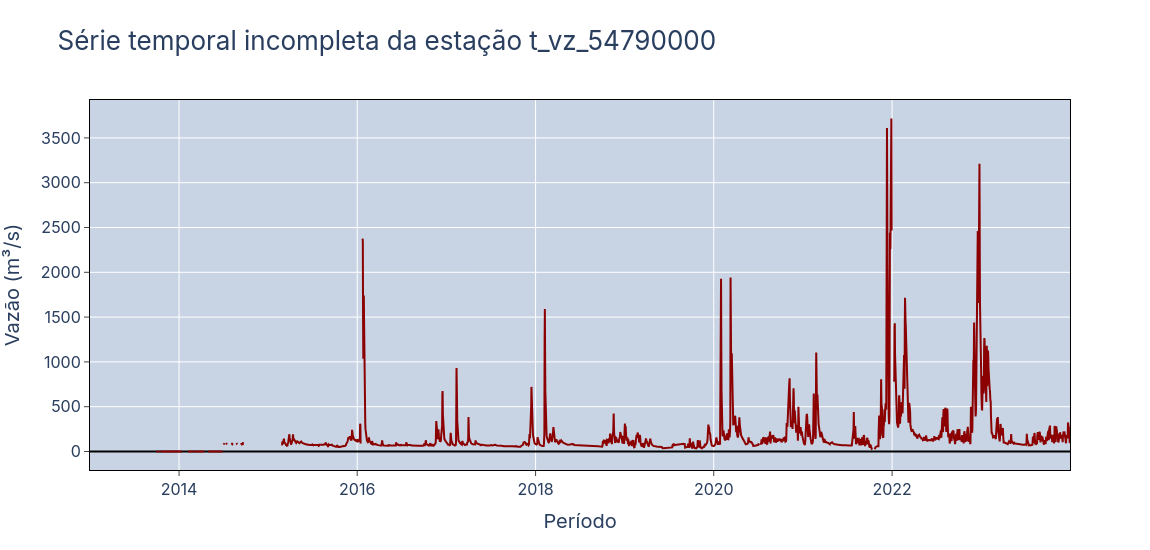
\includegraphics[scale=0.25]{Figuras/jequiti/jequitinhonhaSerieIncompleta_t_vz_54790000.png}
	\caption{Série temporal incompleta da estação t\_vz\_54790000 \\(fonte: o autor)}
	\label{fig:jequitinhonhaSerieIncompleta_t_vz_54790000}
\end{figure}

A seguir, destaca-se o trecho da série com a maior quantidade de dados faltantes (figura \ref{fig:jequitinhonhaSerieIncompleta_t_vz_54790000-2013_2016}), que abrange o período de janeiro de 2013 a janeiro de 2016. Em sequência, é apresentada a série após a imputação dos dados (figura \ref{fig:jequitinhonhaSerieCompleta_t_vz_54790000-2013_2016}). Notavelmente, essa seção não apresentou resultados ideais, uma vez que a imputação atribuiu vazões zero em vários dias, o que não é realista, pois isso indicaria a secagem completa do rio, o que é improvável. No entanto, esses valores zero não impactaram significativamente os resultados finais da análise, já que se referem a um período distante do foco principal deste estudo. Uma alternativa seria excluir todo o trecho anterior ao ano de 2016, mas optou-se por manter a uniformidade nos critérios de aproveitamento dos dados ao longo do trabalho, dado que outros rios também foram analisados, e buscava-se assegurar consistência nos resultados.

\begin{figure}[!h]
	\centering
	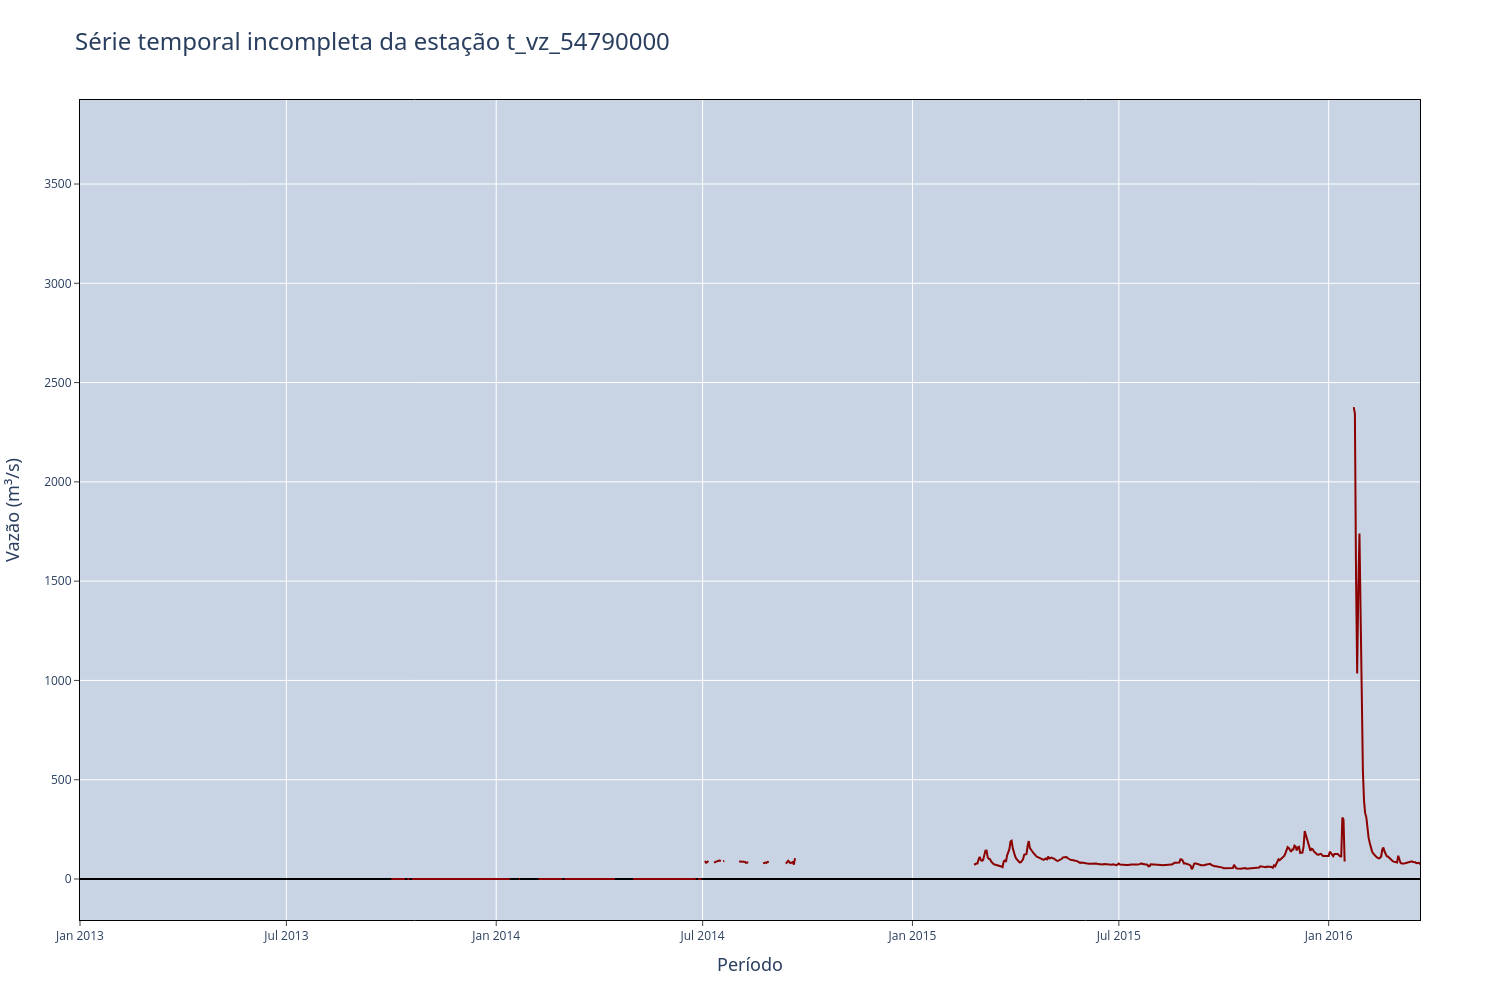
\includegraphics[scale=0.25]{Figuras/jequiti/jequitinhonhaSerieIncompleta_t_vz_54790000-2013_2016.png}
	\caption{Detalhe da série temporal da estação t\_vz\_54790000, ainda sem dados imputados, de 2013 a 2016 (fonte: o autor)}
	\label{fig:jequitinhonhaSerieIncompleta_t_vz_54790000-2013_2016}
\end{figure}

\begin{figure}[!h]
	\centering
	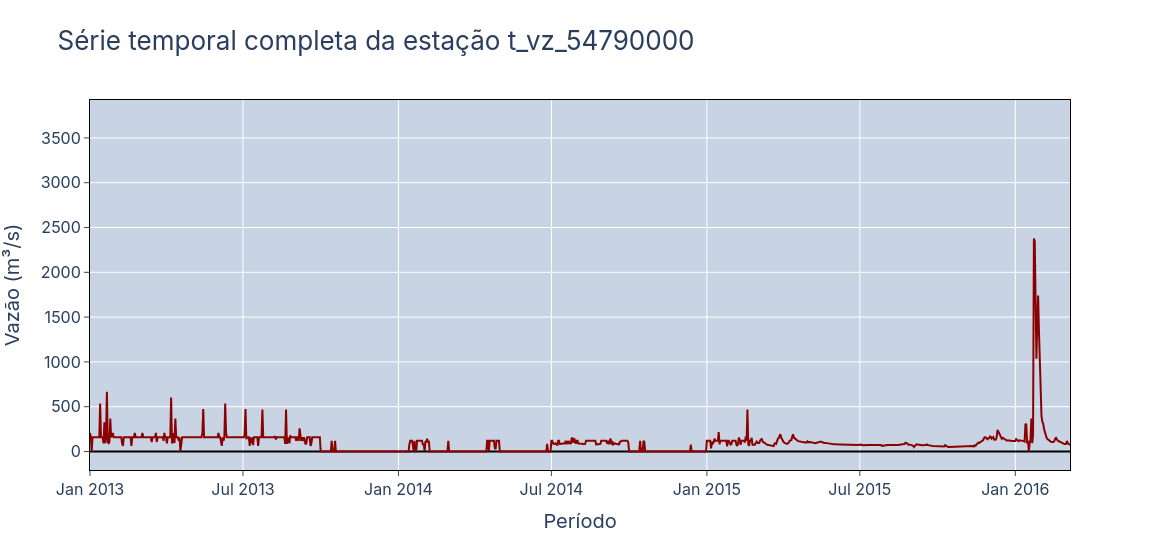
\includegraphics[scale=0.25]{Figuras/jequiti/jequitinhonhaSerieCompleta_t_vz_54790000-2013_2016.png}
	\caption{Detalhe da série temporal da estação t\_vz\_54790000, com dados imputados, de 2013 a 2016 (fonte: o autor)}
	\label{fig:jequitinhonhaSerieCompleta_t_vz_54790000-2013_2016}
\end{figure}

Observe também o trecho de dados faltantes mais próximo ao final dos anos analisados, em 2021 e 2022 (figura \ref{fig:jequitinhonhaSerieIncompleta_t_vz_54790000-2021_2022}). Esta porção da série ficou boa visto que havia informação prévia suficiente, a inserção de dados respeitou coerentemente a sazonalidade (figura \ref{fig:jequitinhonhaSerieCompleta_t_vz_54790000-2021_2022}).

\begin{figure}[!h]
	\centering
	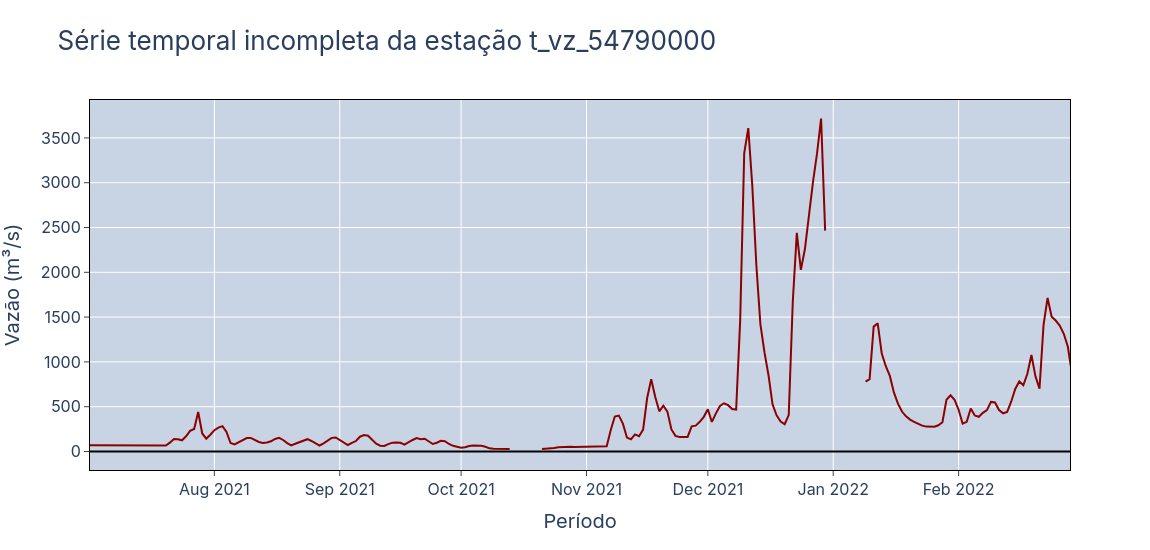
\includegraphics[scale=0.25]{Figuras/jequiti/jequitinhonhaSerieIncompleta_t_vz_54790000-2021_2022.png}
	\caption{Série temporal incompleta da estação t\_vz\_54790000 no detalhe entre 2021 e 2022 (fonte: o autor)}
	\label{fig:jequitinhonhaSerieIncompleta_t_vz_54790000-2021_2022}
\end{figure}

\begin{figure}[!h]
	\centering
	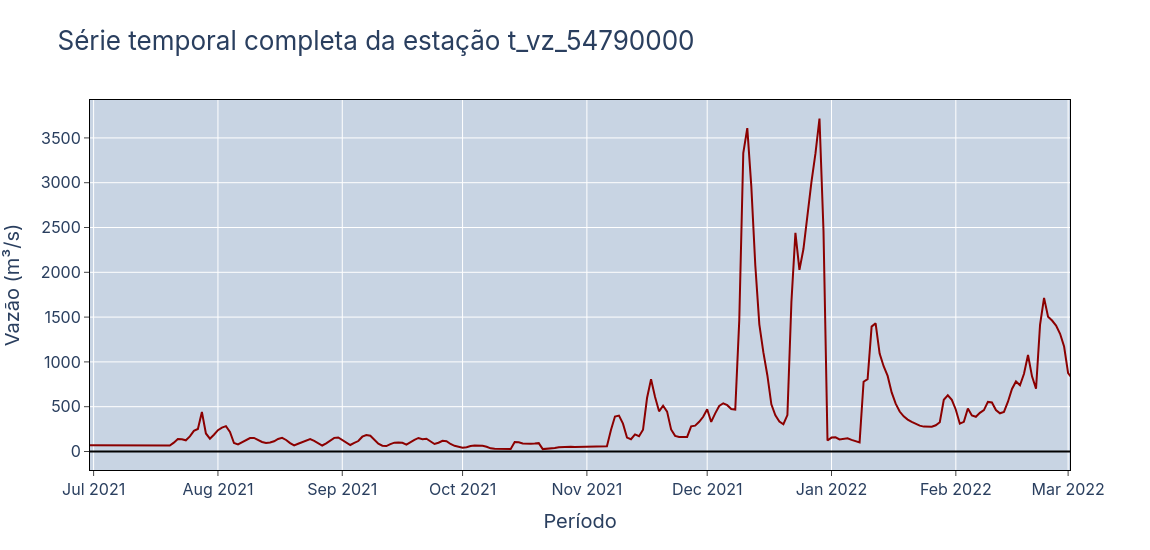
\includegraphics[scale=0.25]{Figuras/jequiti/jequitinhonhaSerieCompleta_t_vz_54790000-2021_2022.png}
	\caption{Série temporal completa da estação t\_vz\_54790000 no detalhe entre 2021 e 2022 (fonte: o autor)}
	\label{fig:jequitinhonhaSerieCompleta_t_vz_54790000-2021_2022}
\end{figure}

Por fim, uma visão ampla de como ficou a série temporal após os procedimentos de imputar os dados. (figura \ref{fig:jequitinhonhaSerieCompleta_t_vz_54790000})

\begin{figure}[!h]
	\centering
	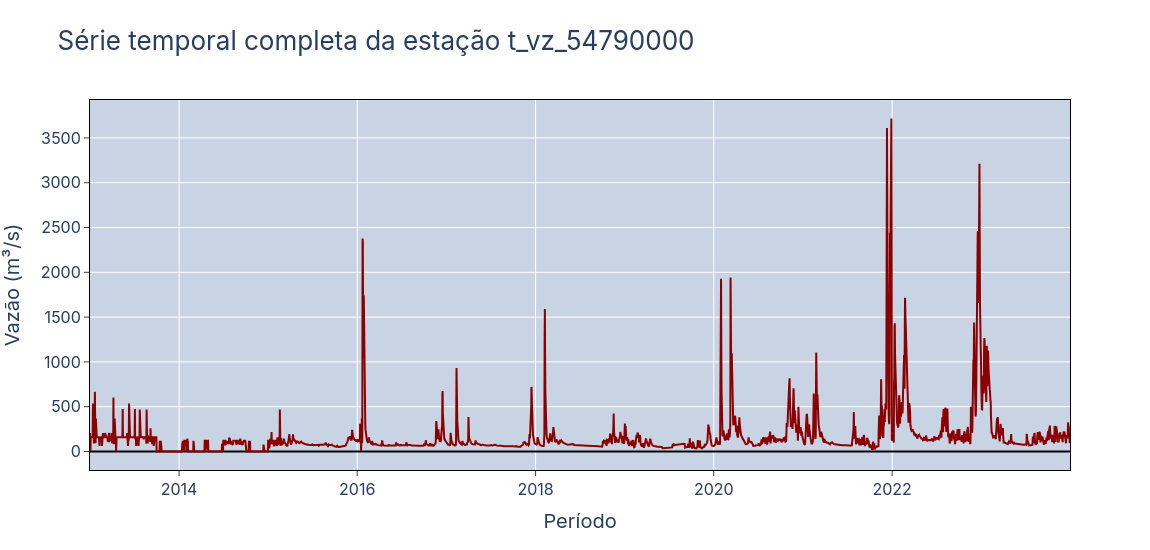
\includegraphics[scale=0.25]{Figuras/jequiti/jequitinhonhaSerieCompleta_t_vz_54790000.png}
	\caption{Série temporal completa da estação t\_vz\_54790000\\(fonte: o autor)}
	\label{fig:jequitinhonhaSerieCompleta_t_vz_54790000}
\end{figure}

A mesma análise foi realizada para as estações de chuva. Na estação t\_cv\_54790000 (figura \ref{fig:jequitinhonhaSerieIncompleta_t_cv_54790000}) faltavam 273 dias de dados (6,79\%). Já a estação t\_cv\_01640000 estava totalmente preenchida, sem valores nulos. (figura \ref{fig:jequitinhonhaSerieCompleta_t_cv_01640000})

\begin{figure}[!h]
	\centering
	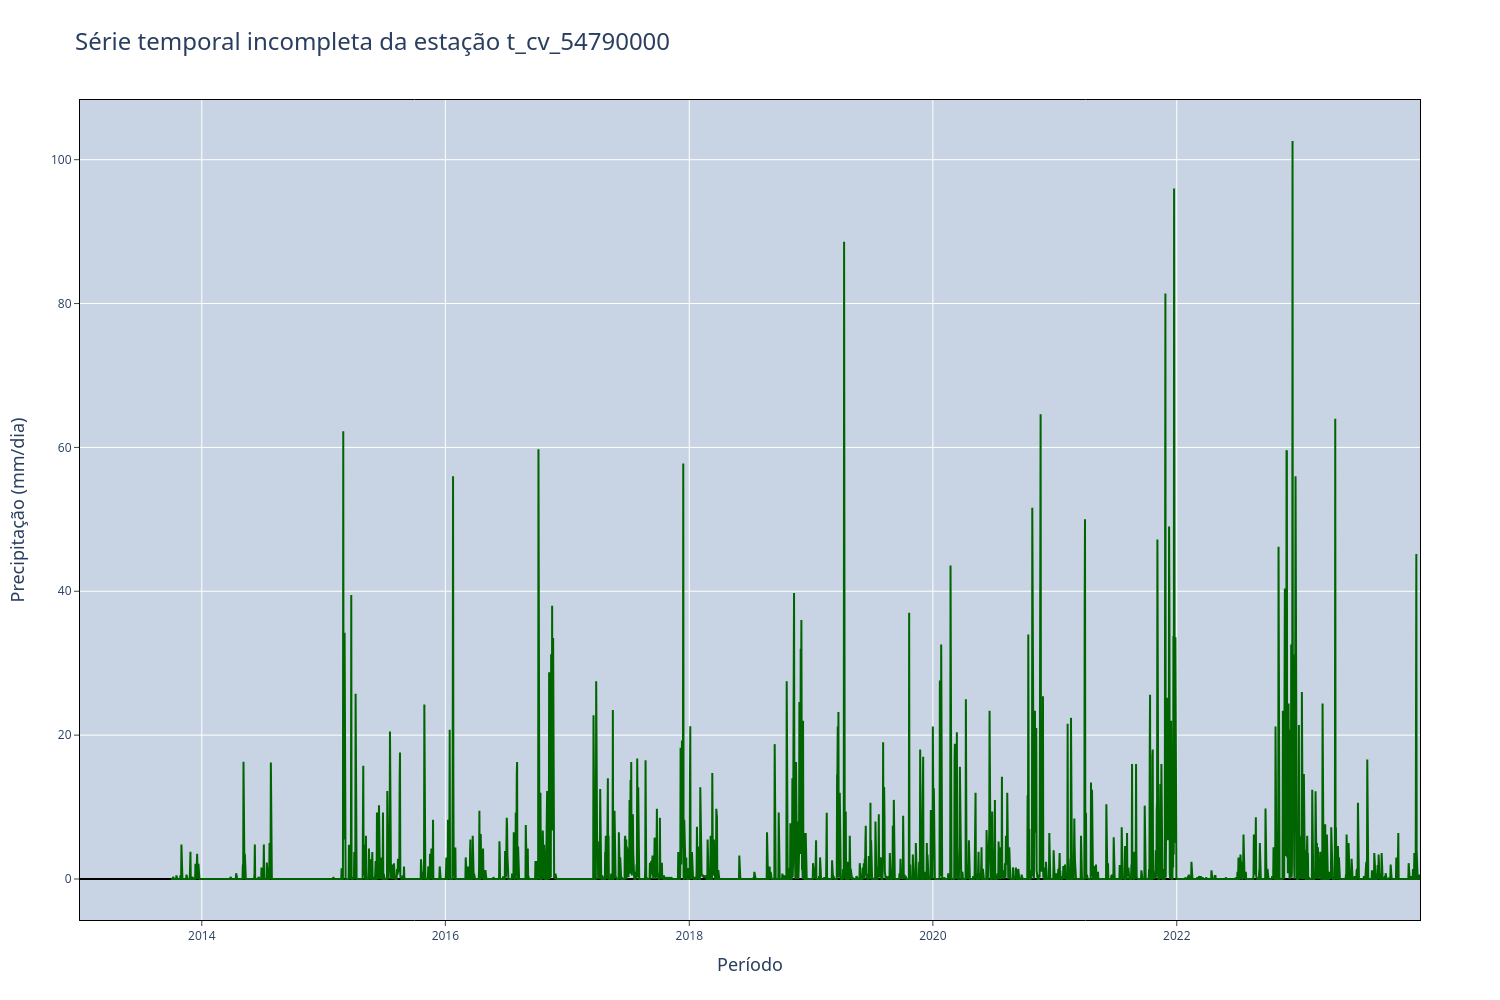
\includegraphics[scale=0.25]{Figuras/jequiti/jequitinhonhaSerieIncompleta_t_cv_54790000.png}
	\caption{Série temporal incompleta da estação t\_cv\_54790000\\(fonte: o autor)}
	\label{fig:jequitinhonhaSerieIncompleta_t_cv_54790000}
\end{figure}

Note que no início desta série de precipitação, o ano de 2013, não possuem dados. As séries de chuva completas ficaram desta forma (figuras \ref{fig:jequitinhonhaSerieCompleta_t_cv_54790000} e \ref{fig:jequitinhonhaSerieCompleta_t_cv_01640000})

\begin{figure}[!h]
	\centering
	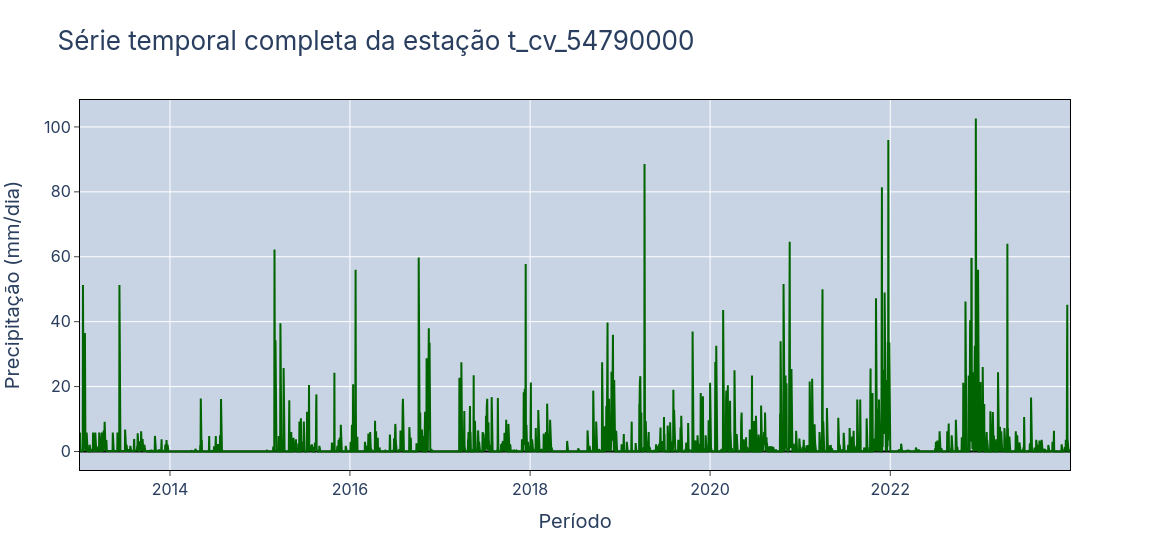
\includegraphics[scale=0.25]{Figuras/jequiti/jequitinhonhaSerieCompleta_t_cv_54790000.png}
	\caption{Série temporal completa da estação t\_cv\_54790000\\(fonte: o autor)}
	\label{fig:jequitinhonhaSerieCompleta_t_cv_54790000}
\end{figure}

\begin{figure}[!h]
	\centering
	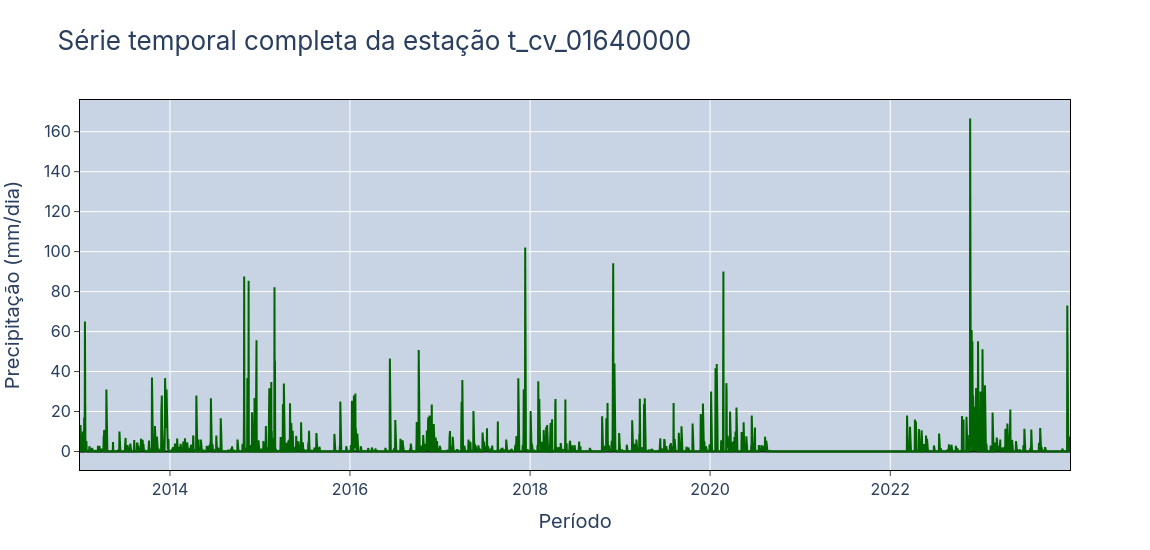
\includegraphics[scale=0.25]{Figuras/jequiti/jequitinhonhaSerieCompleta_t_cv_01640000.png}
	\caption{Série temporal completa da estação t\_cv\_01640000\\(fonte: o autor)}
	\label{fig:jequitinhonhaSerieCompleta_t_cv_01640000}
\end{figure}

\subsection{Rio Doce}

A estação alvo para o rio Doce é a estação c\_vz\_56994500. Sua série temporal foi a que apresentou melhor qualidade no que diz respeito à frequência de medições realizadas. Havia falta de apenas 3 dias, dos 4017 dias do período inteiro. Apenas o preenchimento sazonal bastou para completar a série e não foi preciso mais que isso. Cabe destacar a sazonalidade da série. Ficou bastante evidente este comportamento. (figura \ref{fig:doceSerieCompleta_c_vz_56994500})

\begin{figure}[!h]
	\centering
	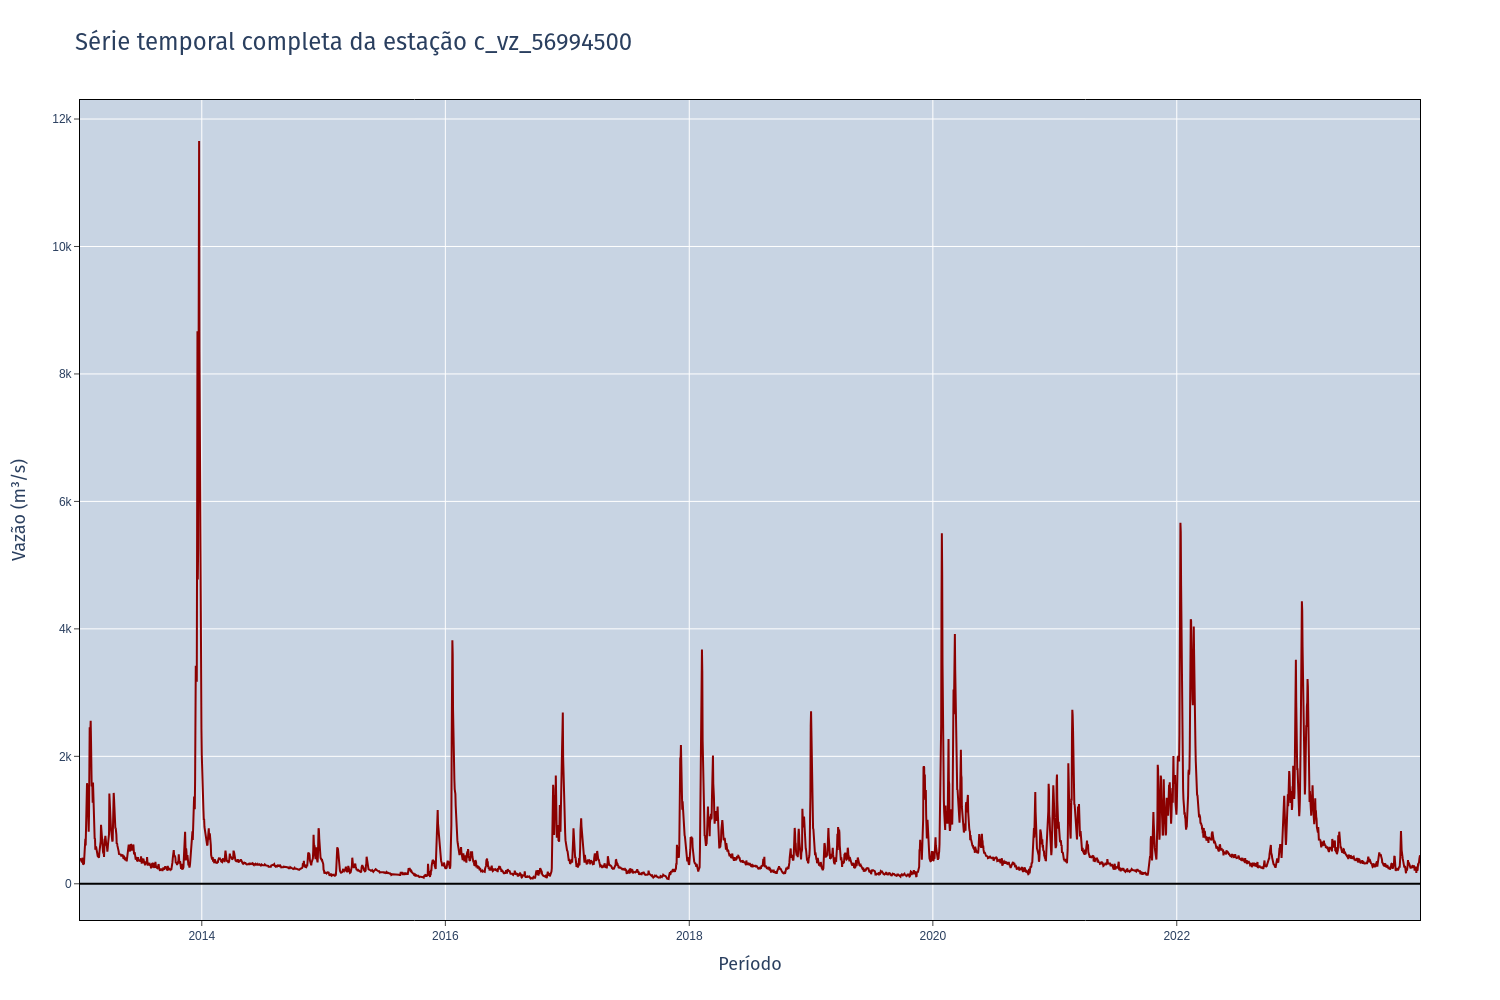
\includegraphics[scale=0.25]{Figuras/rio_doce/doceSerieCompleta_c_vz_56994500.png}
	\caption{Série temporal completa da estação c\_vz\_56994500\\(fonte: o autor)}
	\label{fig:doceSerieCompleta_c_vz_56994500}
\end{figure}

Se para os dados de vazão no rio Doce a série foi, digamos, mais comportada, o mesmo não se pode dizer exatamente das estações de chuva. Ao menos, não para duas delas. Estas estações tiveram os dados desconsiderados e foram removidos das análises. Primeiro foi a estação t\_cv\_56990850 que possuía valores discrepantes demais para serem considerados. Valores da ordem de 7000 mm/dia, 8500 mm/dia. Além deste problema, havia ainda 3134 dias com dados nulos, o que representava 78\% do total. (figura \ref{fig:doceSerieIncompleta_t_cv_56990850})

A outra estação removida foi a t\_cv\_56994500. Conforme pode ser observado na figura \ref{fig:doceSerieCompleta_t_cv_56994500}, nela havia um longo hiato de dados zerados, voltando à normalidade apenas mais recentemente. Como as informações de precipitação que deveria haver para a estação no período do hiato, pode ser retirado de outras estações usadas na modelagem, optou-se por remover esta estação completamente do trabalho.

\begin{figure}[!h]
	\centering
	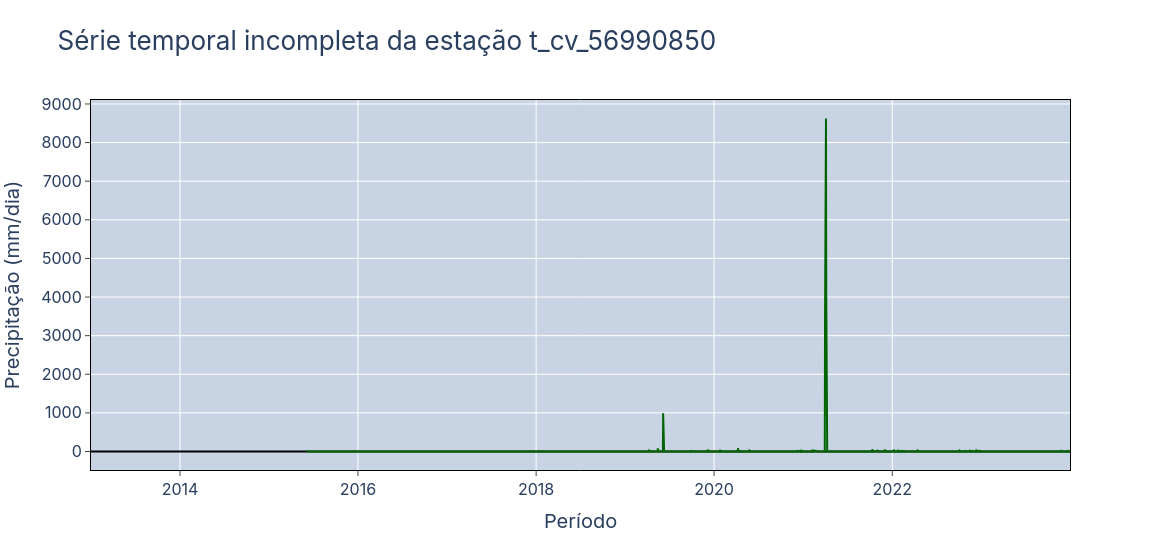
\includegraphics[scale=0.25]{Figuras/rio_doce/doceSerieIncompleta_t_cv_56990850.png}
	\caption{Série temporal da estação t\_cv\_56990850 - não utilizada\\(fonte: o autor)}
	\label{fig:doceSerieIncompleta_t_cv_56990850}
\end{figure}

\begin{figure}[!h]
	\centering
	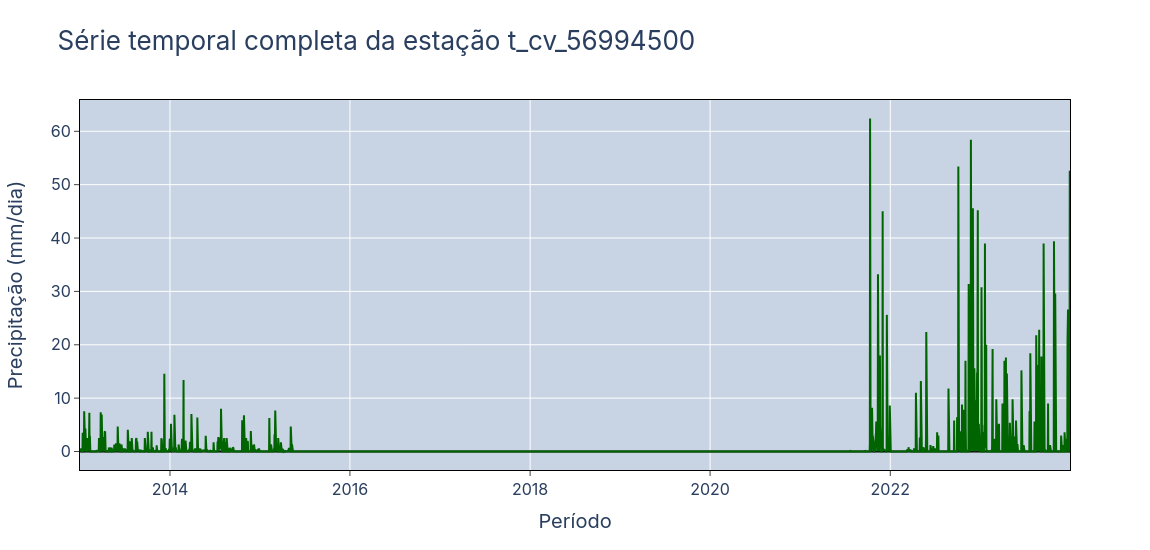
\includegraphics[scale=0.25]{Figuras/rio_doce/doceSerieCompleta_t_cv_56994500.png}
	\caption{Série temporal da estação t\_cv\_56994500 - não utilizada\\(fonte: o autor)}
	\label{fig:doceSerieCompleta_t_cv_56994500}
\end{figure}

As estações que, enfim, foram empregadas na modelagem são as que estão na tabela e, adiante, o gráfico da série temporal de cada uma delas. (figuras \ref{fig:doceSerieCompleta_c_cv_01941010}, \ref{fig:doceSerieCompleta_c_cv_01941004}, \ref{fig:doceSerieCompleta_c_cv_01941006} e \ref{fig:doceSerieCompleta_t_cv_56990005})

\begin{table}[h!]
	\centering \small
	\caption{Estações de precipitação usadas - final \\(fonte: o autor)}
	\begin{tabular}{|c|c|c|} \hline
		\textbf{Estação} & \textbf{\# dados faltantes} & \textbf{\% dados faltantes} \\ \hline
		c\_cv\_01941010  & 153                         & 3,81 \\ \hline
		c\_cv\_01941004  & 31                          & 0,77 \\ \hline
		c\_cv\_01941006  & 0                           & 0,00 \\ \hline
		t\_cv\_56990005  & 1395                        & 34,73 \\ \hline
	\end{tabular}
	\label{tab:estacoes_chuva_usadas_final_rio_doce}
\end{table}

\begin{figure}[!h]
	\centering
	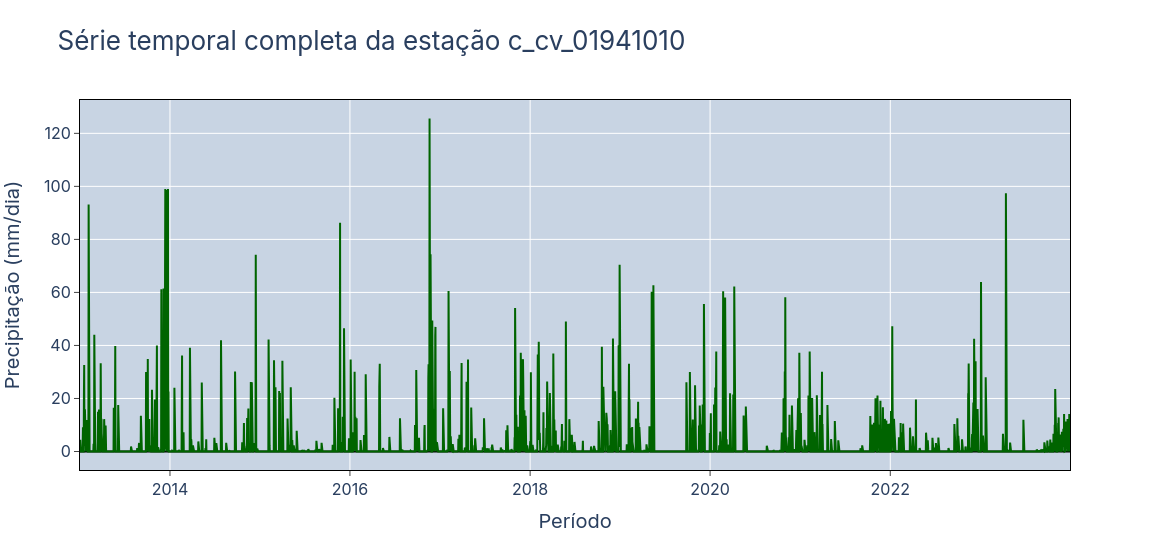
\includegraphics[scale=0.25]{Figuras/rio_doce/doceSerieCompleta_c_cv_01941010.png}
	\caption{Série temporal completa da estação c\_cv\_01941010\\(fonte: o autor)}
	\label{fig:doceSerieCompleta_c_cv_01941010}
\end{figure}

\begin{figure}[!h]
	\centering
	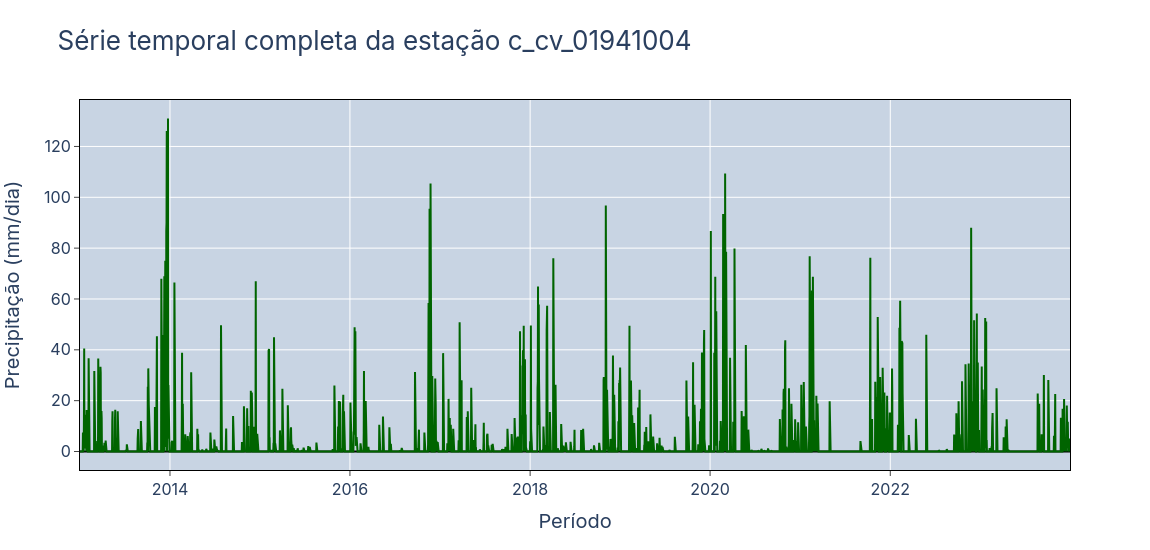
\includegraphics[scale=0.25]{Figuras/rio_doce/doceSerieCompleta_c_cv_01941004.png}
	\caption{Série temporal completa da estação c\_cv\_01941004\\(fonte: o autor)}
	\label{fig:doceSerieCompleta_c_cv_01941004}
\end{figure}

\begin{figure}[!h]
	\centering
	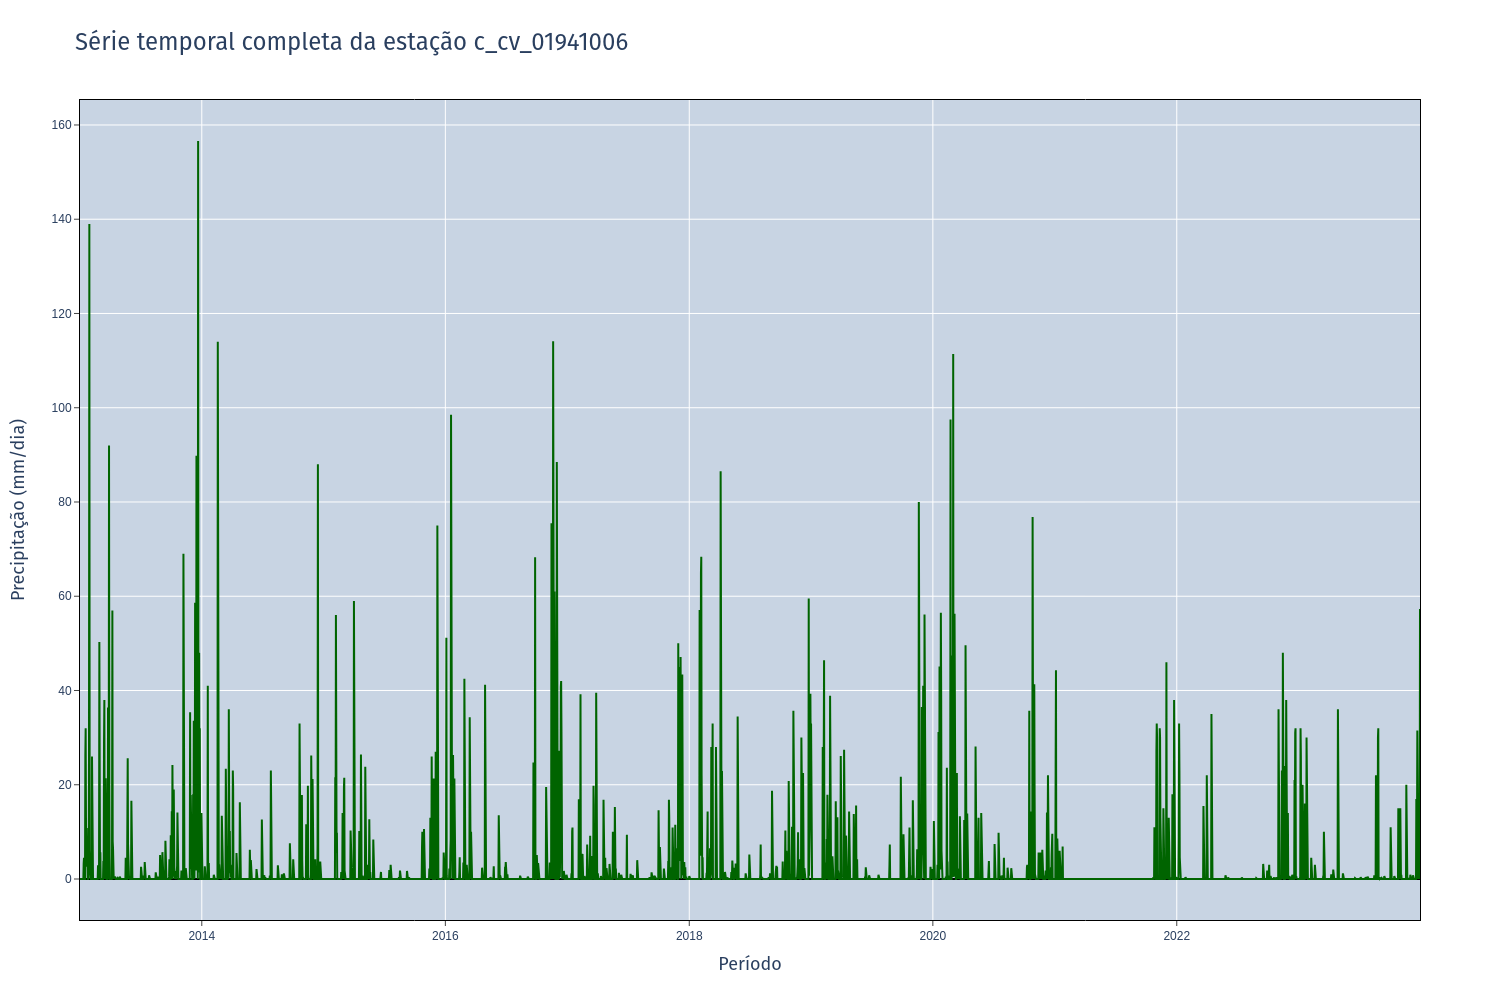
\includegraphics[scale=0.25]{Figuras/rio_doce/doceSerieCompleta_c_cv_01941006.png}
	\caption{Série temporal completa da estação c\_cv\_01941006\\(fonte: o autor)}
	\label{fig:doceSerieCompleta_c_cv_01941006}
\end{figure}

\begin{figure}[!h]
	\centering
	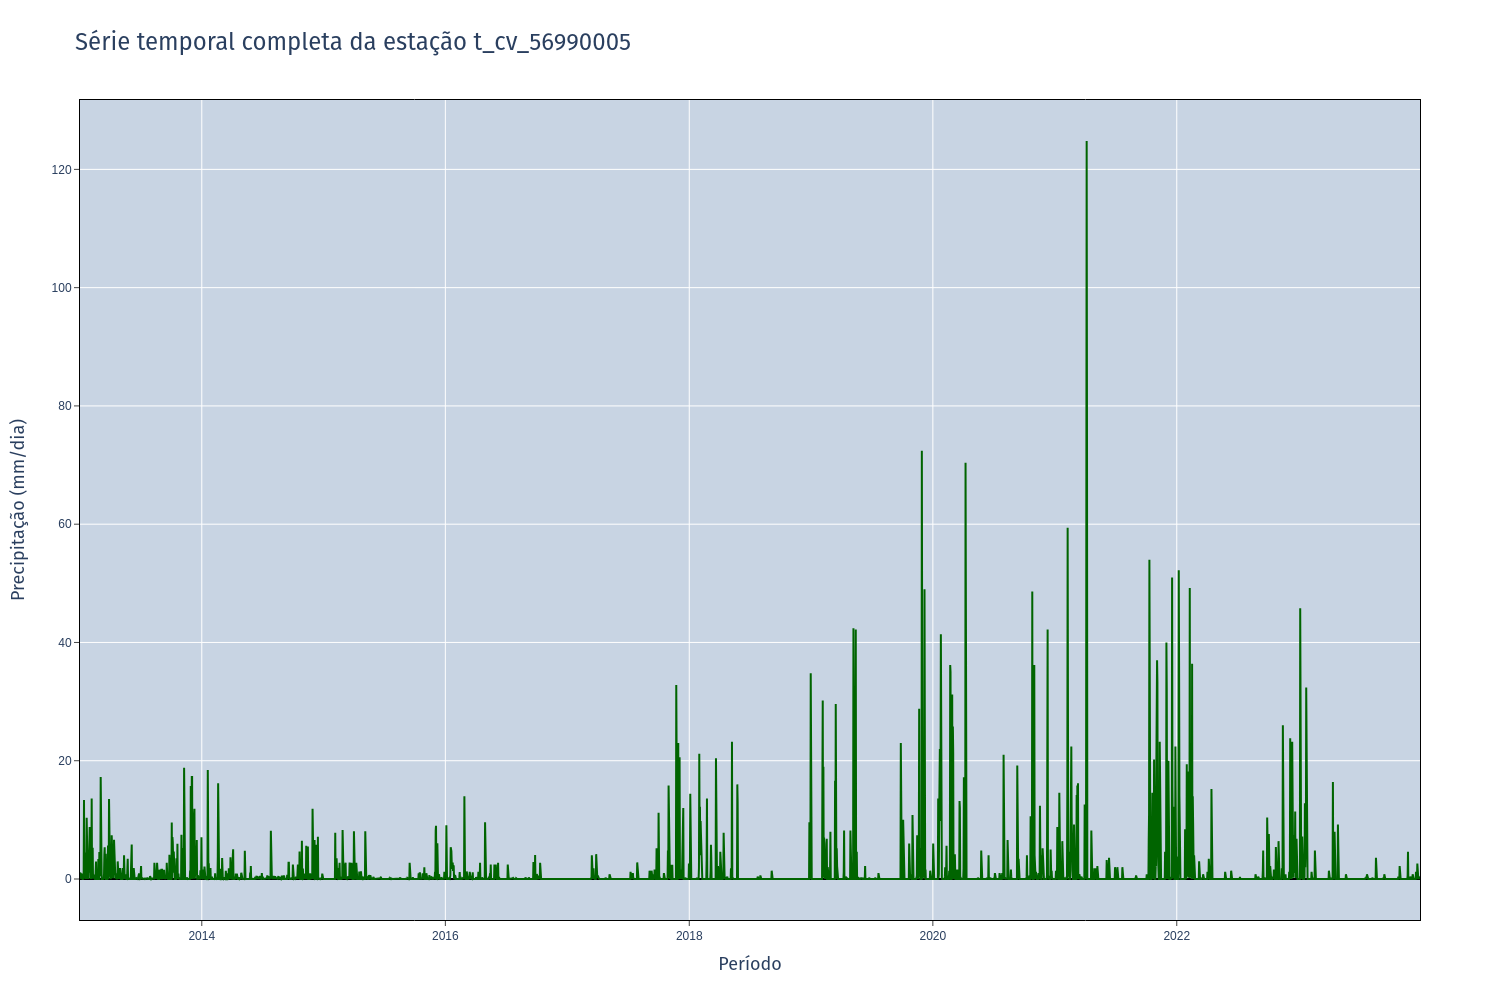
\includegraphics[scale=0.25]{Figuras/rio_doce/doceSerieCompleta_t_cv_56990005.png}
	\caption{Série temporal completa da estação t\_cv\_56990005\\(fonte: o autor)}
	\label{fig:doceSerieCompleta_t_cv_56990005}
\end{figure}

\clearpage
\subsection{Rio Grande}

O rio Grande apresentou desafios significativos ao longo de todo o desenvolvimento deste trabalho. A dificuldade inicial surgiu na ausência de dados disponíveis em estações dentro do estado de Minas Gerais para o período de análise estipulado, conforme mencionado anteriormente. Foi necessário buscar uma estação o mais próxima possível da divisa com Minas Gerais, localizada no estado de São Paulo, especificamente no município de Ilha Solteira. Entretanto, os desafios não se limitaram a essa questão geográfica.

A série temporal de vazão da estação selecionada, denominada t\_vz\_62020080, estava incompleta e não abrangia todo o período de 11 anos estipulado para a análise. (figura \ref{fig:grandeSerieIncompleta_t_vz_62020080}) Os dados disponíveis mais antigos datavam de 2020. Contudo, em conformidade com o escopo estabelecido para este estudo, foi realizado o preenchimento dos dados faltantes, aplicando-se o mesmo protocolo utilizado para os demais rios analisados. Este procedimento foi necessário para garantir a consistência, integridade e comparabilidade das análises subsequentes.

\begin{figure}[!h]
	\centering
	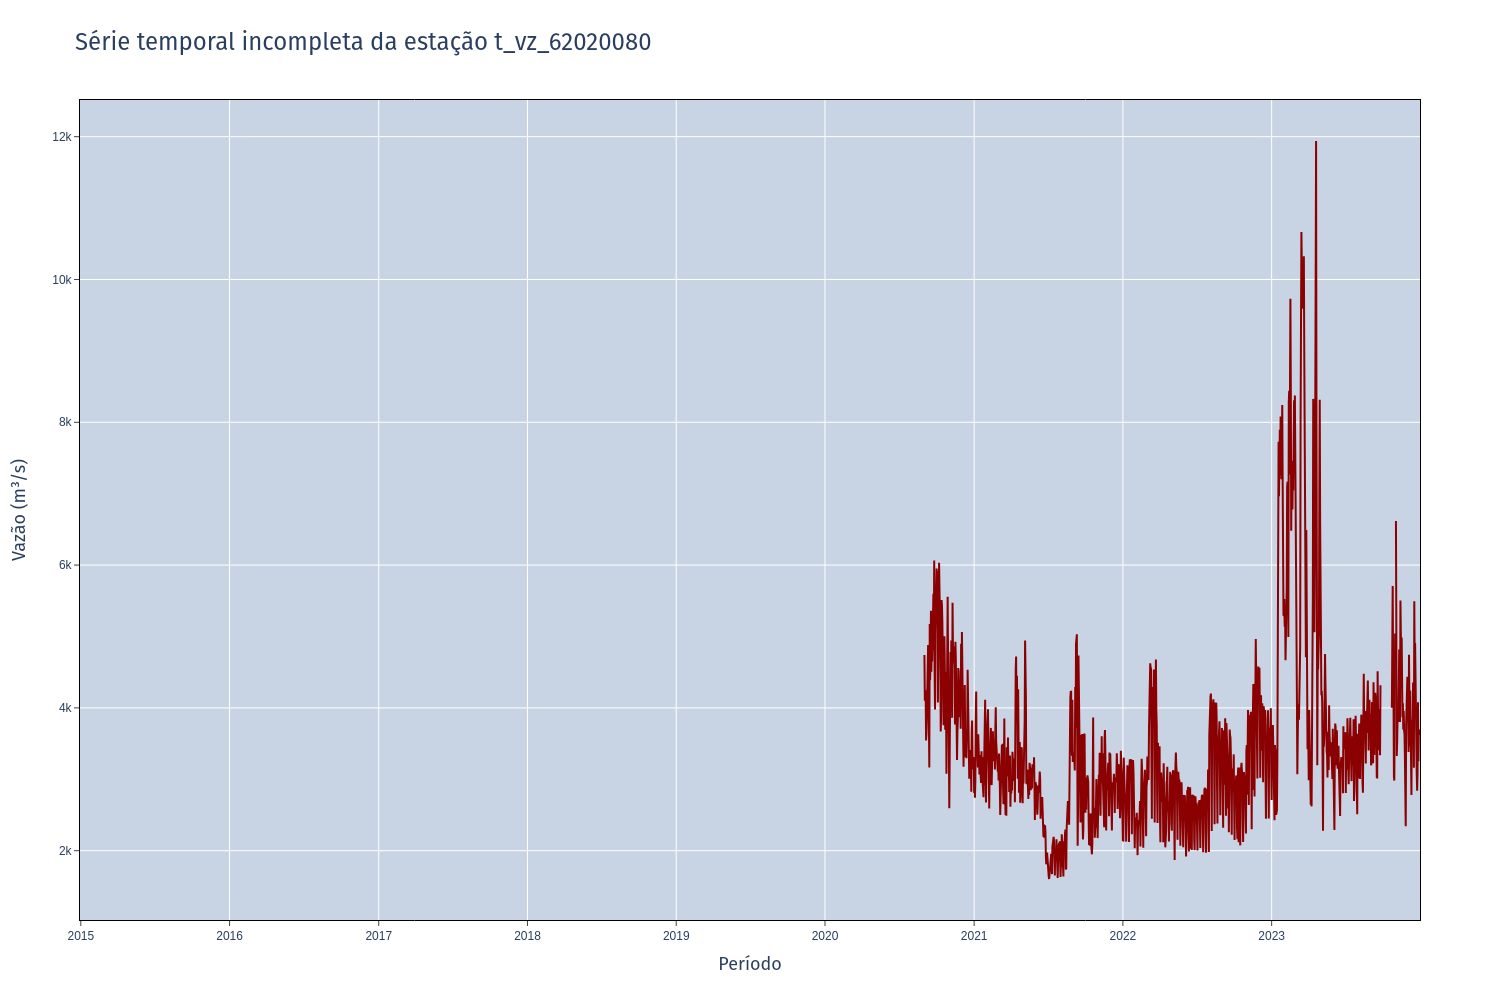
\includegraphics[scale=0.25]{Figuras/rio_grande/grandeSerieIncompleta_t_vz_62020080.png}
	\caption{Série temporal incompleta da estação t\_vz\_62020080\\(fonte: o autor)}
	\label{fig:grandeSerieIncompleta_t_vz_62020080}
\end{figure}

Infelizmente, o caráter ruidoso da série permaneceu mesmo após a aplicação do protocolo de preenchimento dos dados ausentes, conforme pode ser observado na imagem final gerada.(figura \ref{fig:grandeSerieCompleta_t_vz_62020080}) A série em questão apresentava 2099 dias faltantes, correspondendo a aproximadamente 64\% de dados nulos. Outro aspecto relevante para essa estação é que, diferentemente das outras, não foram utilizados os 4.017 registros previstos inicialmente. As informações mais antigas disponíveis datavam de 2015, resultando, assim, em um total de 3289 registros diários utilizados especificamente para o rio Grande.

\begin{figure}[!h]
	\centering
	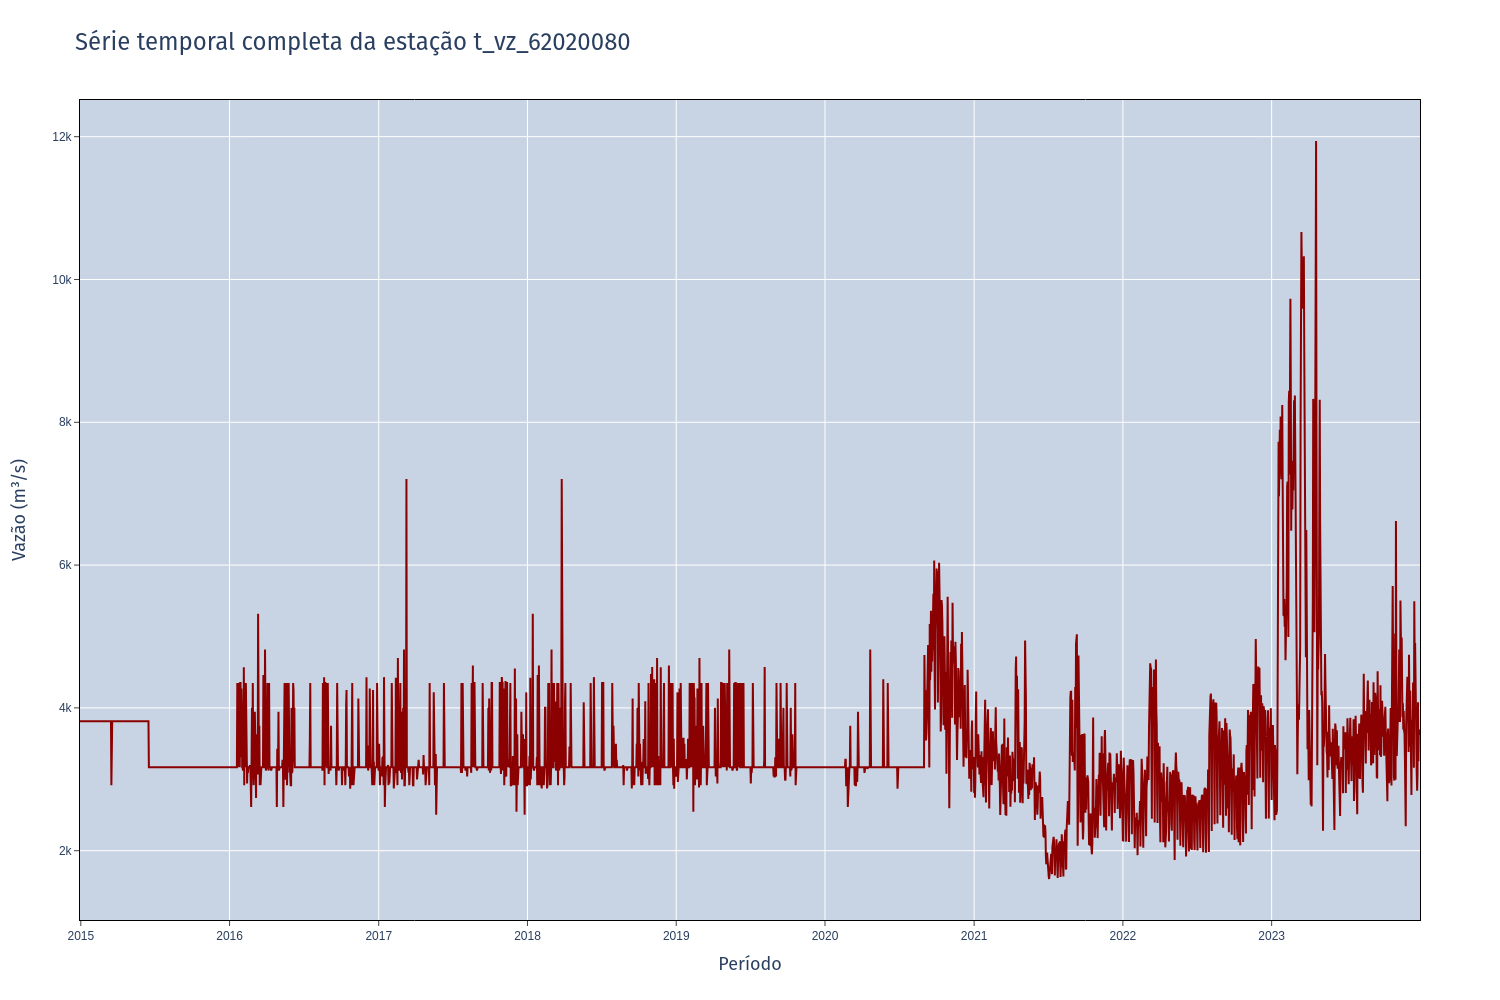
\includegraphics[scale=0.25]{Figuras/rio_grande/grandeSerieCompleta_t_vz_62020080.png}
	\caption{Série temporal completa da estação t\_vz\_62020080\\(fonte: o autor)}
	\label{fig:grandeSerieCompleta_t_vz_62020080}
\end{figure}

A estação de precipitação utilizada, a única neste caso, foi a estação t\_cv\_61998080, pois foi a única que apresentou dados válidos. Curiosamente, outra estação de precipitação disponível também apresentou dados para o período analisado, mas a base de dados consistia exclusivamente em valores zero. Por essa razão, a estação t\_cv\_62020080 foi completamente excluída do estudo.

Em relação à estação t\_cv\_61998080, houve necessidade de preencher apenas um número reduzido de dados ausentes, totalizando 169 registros, o que correspondia a 5,14\% do total. (figura \ref{fig:grandeSerieCompleta_t_cv_61998080}) Trata-se de uma série com uma quantidade expressiva de dados, que efetivamente pôde contribuir de maneira significativa para as análises realizadas.

\begin{figure}[!h]
	\centering
	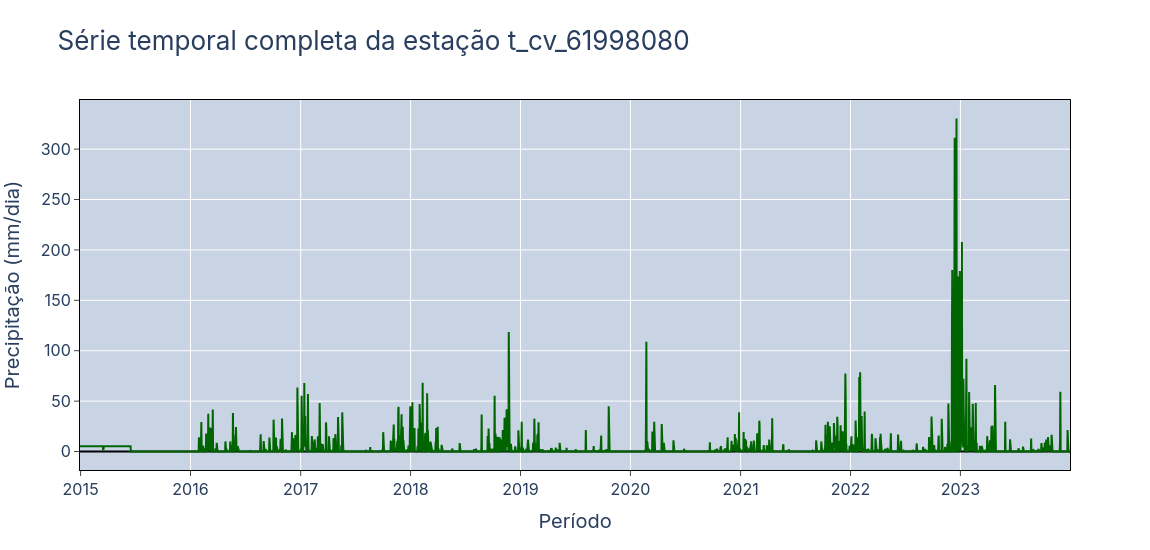
\includegraphics[scale=0.25]{Figuras/rio_grande/grandeSerieCompleta_t_cv_61998080.png}
	\caption{Série completa da estação t\_cv\_61998080\\(fonte: o autor)}
	\label{fig:grandeSerieCompleta_t_cv_61998080}
\end{figure}

Ressalta-se que o trecho de dados faltantes para a estação t\_cv\_61998080 concentrava-se no início da série temporal, especificamente no ano de 2015. No gráfico os dados já estão imputados.

\clearpage
\subsection{Rio São Francisco}

Por fim, foi realizado o procedimento de preenchimento dos dados nulos para o rio São Francisco. A estação-alvo c\_vz\_44290002 apresentou uma série bastante completa ao longo do período de análise, com apenas 120 dias nulos em um total de 4017 dias. O trecho com dados faltantes pode ser observado em detalhe na figura (\ref{fig:franciscoSerieIncompleta_c_vz_44290002-detalhe}).

Para esta estação, o preenchimento sazonal foi suficiente para suprir as lacunas existentes, não sendo necessário aplicar procedimentos adicionais de imputação de dados. (figura \ref{fig:franciscoSerieCompleta_c_vz_44290002})

\begin{figure}[!h]
	\centering
	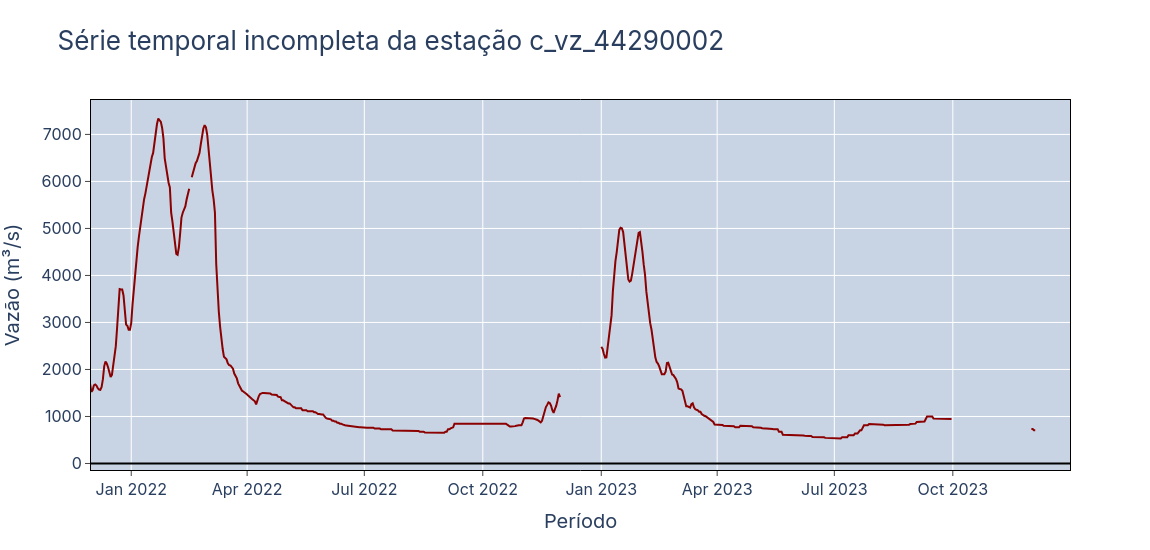
\includegraphics[scale=0.25]{Figuras/rio_sao_francisco/franciscoSerieIncompleta_c_vz_44290002-detalhe.png}
	\caption{Detalhe do trecho com dados nulos da estação c\_vz\_44290002\\(fonte: o autor)}
	\label{fig:franciscoSerieIncompleta_c_vz_44290002-detalhe}
\end{figure}

\begin{figure}[!h]
	\centering
	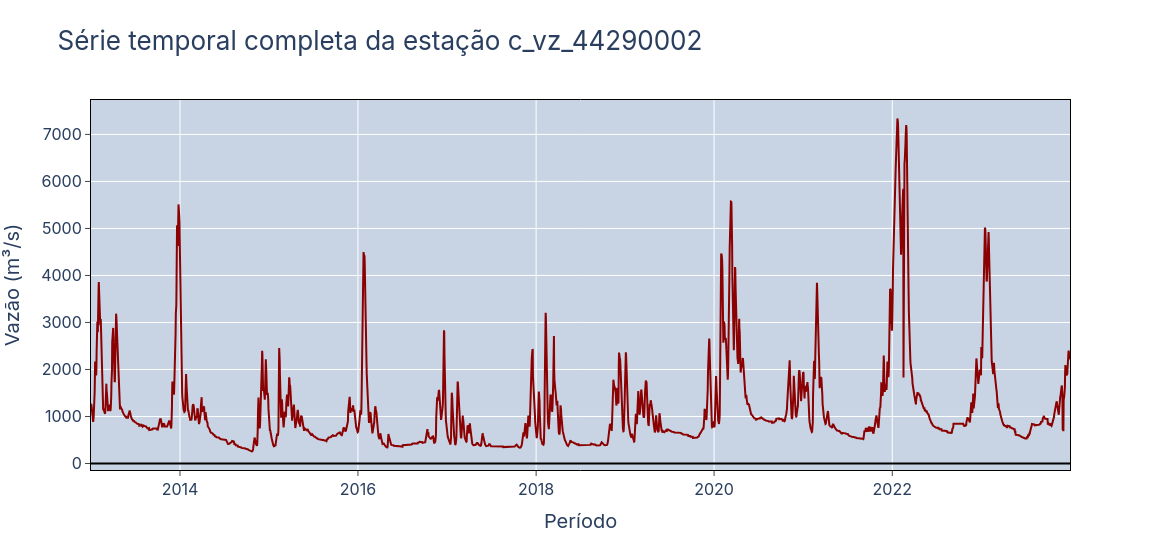
\includegraphics[scale=0.25]{Figuras/rio_sao_francisco/franciscoSerieCompleta_c_vz_44290002.png}
	\caption{Série temporal completa da estação c\_vz\_44290002\\(fonte: o autor)}
	\label{fig:franciscoSerieCompleta_c_vz_44290002}
\end{figure}
\clearpage

No que se refere às estações de precipitação selecionadas para a análise no rio São Francisco, não foi necessário realizar nenhuma inserção de dados, uma vez que todas as séries estavam completas, abrangendo a totalidade dos 4017 dias de registro. As séries temporais correspondentes podem ser visualizadas nos gráficos apresentados a seguir. (figuras \ref{fig:franciscoSerieCompleta_c_cv_01544017}, \ref{fig:franciscoSerieCompleta_c_cv_01544032}, \ref{fig:franciscoSerieCompleta_c_cv_01544036})

\begin{figure}[!h]
	\centering
	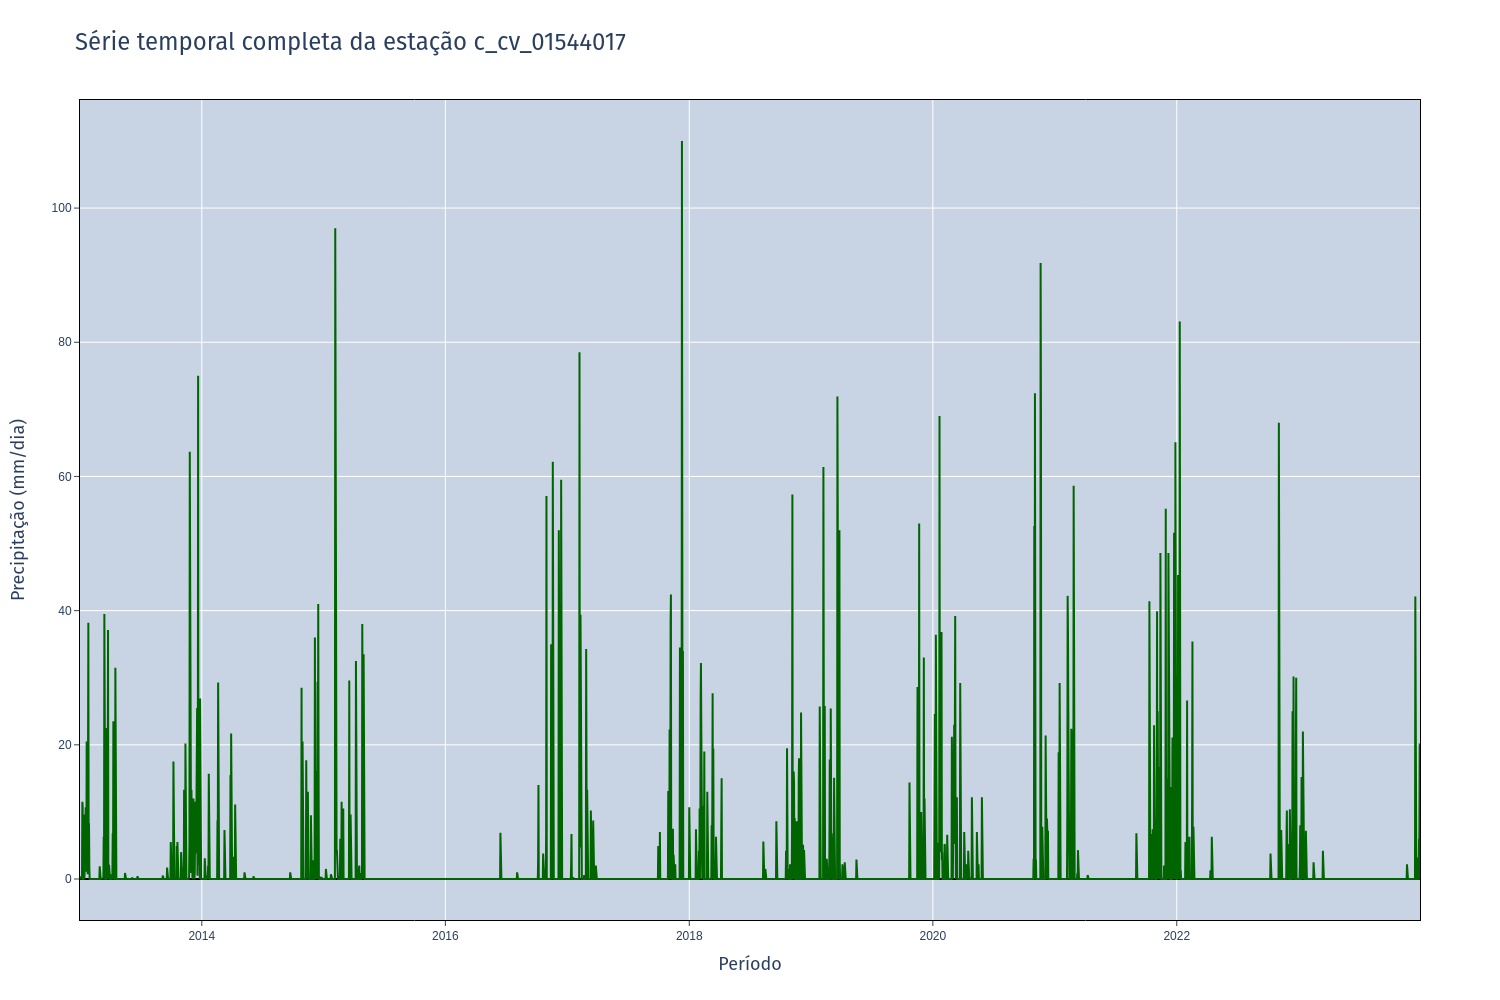
\includegraphics[scale=0.25]{Figuras/rio_sao_francisco/franciscoSerieCompleta_c_cv_01544017.png}
	\caption{Série temporal completa da estação c\_cv\_01544017\\(fonte: o autor)}
	\label{fig:franciscoSerieCompleta_c_cv_01544017}
\end{figure}

\begin{figure}[!h]
	\centering
	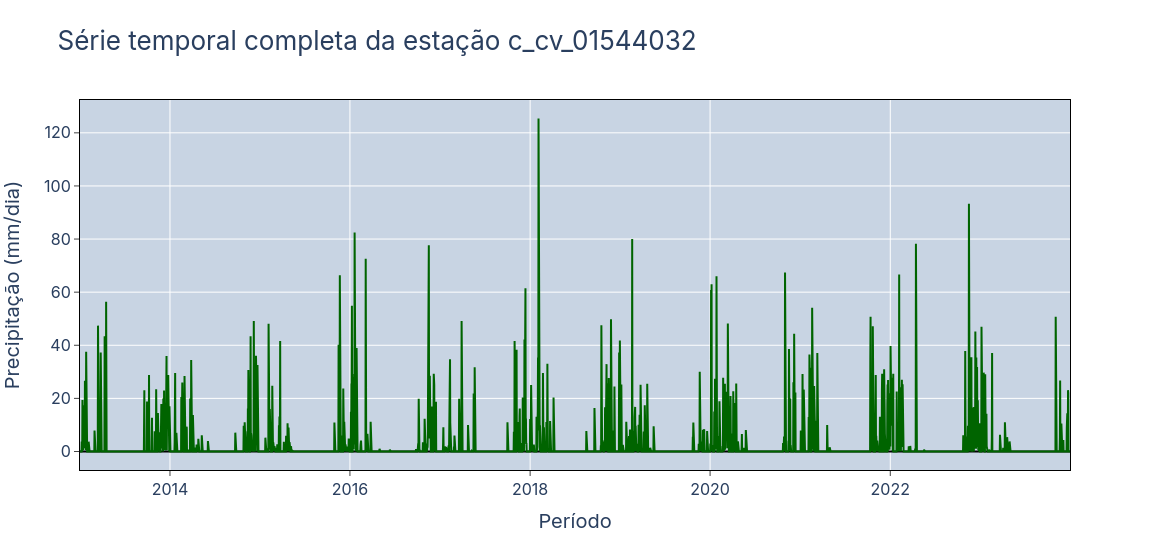
\includegraphics[scale=0.25]{Figuras/rio_sao_francisco/franciscoSerieCompleta_c_cv_01544032.png}
	\caption{Série temporal completa da estação c\_cv\_01544032\\(fonte: o autor)}
	\label{fig:franciscoSerieCompleta_c_cv_01544032}
\end{figure}

\begin{figure}[!h]
	\centering
	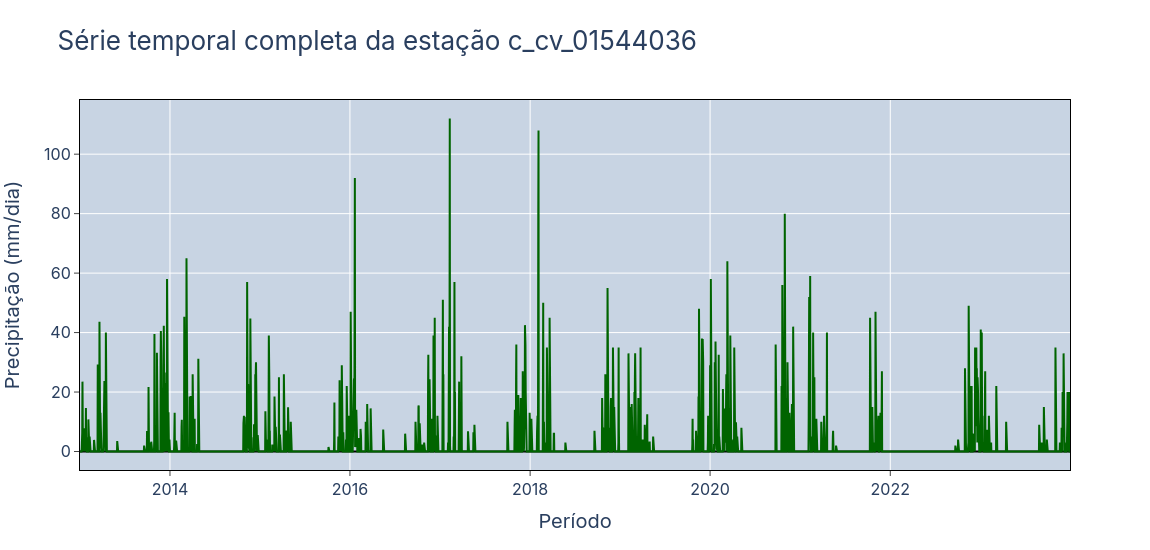
\includegraphics[scale=0.25]{Figuras/rio_sao_francisco/franciscoSerieCompleta_c_cv_01544036.png}
	\caption{Série temporal completa da estação c\_cv\_01544036\\(fonte: o autor)}
	\label{fig:franciscoSerieCompleta_c_cv_01544036}
\end{figure}
\clearpage

\section{Variáveis Utilizadas}
%Listar e explicar as variáveis contínuas e categóricas utilizadas nos modelos.

As variáveis do trabalho, exceto as categóricas, obviamente, são todas contínuas. Todas as séries temporais foram ajustadas para estarem completas dentro do período trabalhado, totalizando 4017 registros diários. A exceção ficou por conta dos dados do rio Grande, em que o dado mais antigo foi o dia 30 de dezembro de 2014.

Para que se tenha uma noção melhor, abaixo seguem alguns dados estatísticos relevantes que informam sobre os dados de vazão e precipitação utilizados. Conste-se que as unidades de precipitação estão em mm/dia e vazão em $m^3/s$.

\begin{table}[!h]
	\centering \small
	\caption{Variáveis utilizadas - rio Jequitinhonha \\(fonte: o autor)}
	\begin{tabular}{|l|r|r|r|r|r|r|} \hline 
		\textbf{Variável}   & \textbf{\#} & \textbf{Média} & \textbf{Desvio-padrão} & \textbf{Mín} & \textbf{< 50\%} & \textbf{Máx} \\\hline
		t\_cv\_01640000     & 4017        & 1,58           & 6,85                   & 0,00         & 0,00            & 166,60       \\\hline
		t\_cv\_54790000     & 4017        & 1,68           & 6,31                   & 0,00         & 0,00            & 102,60       \\\hline
		t\_vz\_54790000 (y) & 4017        & 160,95         & 267,90                 & 0,00         & 95,95           & 3716,65      \\\hline
	\end{tabular}
	\label{tab:variaveis_jequitinhonha}
\end{table}

\begin{table}[!h]
	\centering \small
	\caption{Variáveis utilizadas - rio Doce \\(fonte: o autor)}
	\begin{tabular}{|l|r|r|r|r|r|r|} \hline 
		\textbf{Variável}   & \textbf{\#} & \textbf{Média} & \textbf{Desvio-padrão} & \textbf{Mín} & \textbf{< 50\%} & \textbf{Máx} \\\hline
		c\_cv\_01941010     & 4017        & 2,21           & 8,41                   & 0,00         & 0,00            & 125,60       \\\hline
		c\_cv\_01941004     & 4017        & 2,59           & 9,83                   & 0,00         & 0,00            & 131,00       \\\hline
		c\_cv\_01941006     & 4017        & 2,44           & 9,76                   & 0,00         & 0,00            & 156,60       \\\hline
		t\_cv\_56990005     & 4017        & 1,15           & 5,19                   & 0,00         & 0,00            & 124,80       \\\hline
		c\_vz\_56994500 (y) & 4017        & 542,05         & 656,99                 & 75,15        & 341,26          & 11655,20     \\\hline
	\end{tabular}
	\label{tab:variaveis_rio_doce}
\end{table}

\begin{table}[!h]
	\centering \small
	\caption{Variáveis utilizadas - rio Grande \\(fonte: o autor)}
	\begin{tabular}{|l|r|r|r|r|r|r|} \hline 
		\textbf{Variável}   & \textbf{\#} & \textbf{Média} & \textbf{Desvio-padrão} & \textbf{Mín} & \textbf{< 50\%} & \textbf{Máx} \\\hline
		t\_cv\_61998080     & 3289        & 3,13           & 13,92                  & 0,00         & 0,00            & 330,40       \\\hline
		t\_vz\_62020080 (y) & 3289        & 3405,27        & 873,88                 & 1603,58      & 3170,08         & 11939,49     \\\hline
	\end{tabular}
	\label{tab:variaveis_rio_grande}
\end{table}

\begin{table}[!h]
	\centering \small
	\caption{Variáveis utilizadas - rio São Francisco \\(fonte: o autor)}
	\begin{tabular}{|l|r|r|r|r|r|r|} \hline 
		\textbf{Variável}   & \textbf{\#} & \textbf{Média} & \textbf{Desvio-padrão} & \textbf{Mín} & \textbf{< 50\%} & \textbf{Máx} \\\hline
		c\_cv\_01544017     & 4017        & 1,60           & 7,39                   & 0,00         & 0,00            & 110,00       \\\hline
		c\_cv\_01544032     & 4017        & 2,30           & 8,13                   & 0,00         & 0,00            & 125,40       \\\hline
		c\_cv\_01544036     & 4017        & 1,99           & 7,59                   & 0,00         & 0,00            & 112,00       \\\hline
		c\_vz\_44290002 (y) & 4017        & 1115,88        & 998,40                 & 254,75       & 812,26          & 7338,65      \\\hline
	\end{tabular}
	\label{tab:variaveis_rio_sao_francisco}
\end{table}
\clearpage

É possível identificar algumas questões importantes sobre a massa de dados a partir destas tabelas. Observe que para o rio Jequitinhonha (tabela \ref{tab:variaveis_jequitinhonha}) a vazão mínima foi 0,00 $m^3/s$, o que denotaria que o rio passou por um período de seca. Porém não foi encontrado, seja em artigos científicos sobre o rio, quanto em matérias de jornais, que o rio Jequitinhonha tenha passado por isso no período analisado. Não é de se surpreender, contudo, que estes valores zero tenham sido inseridos quando da imputação dos dados, visto que este trecho da série temporal era onde estava a maior lacuna. No entanto, não foi feita substituição dos valores zero por, por exemplo, a média de vazão. Problemas com falta de dados e crítica quanto aos dados inseridos não foram feitas. Estas e outras incertezas que permearam todas análises foram, onde puder e couber, discutidas, mas manteve-se o trabalho mesmo com estas questões levantadas, sem fazer um tratamento específico. Uma observação geral sobre os dados de vazão é que existe uma amplitude elevada entre o mínimo e o máximo, em todas as estações utilizadas, com uma pequena variação para o rio Grande. Contudo, com este rio especificamente, os dados de vazão tiveram alguns problemas e dificuldades e é provável que estes números não estejam coerentes com a realidade. Mas o rio Doce é realmente considerável. (tabela \ref{tab:variaveis_rio_doce}) Vale destacar, no entanto, que esta amplitude não especifica se foi dentro de um ano. É ao longo de toda série temporal, ou seja, ao longo dos 11 anos de dados considerados.

As variáveis de precipitação, mesmo considerando o somatório diário de precipitação, tiveram muitos dados zero. Nota-se isso a partir da análise da coluna ``< 50\%'', que significa metade de toda massa de dados de precipitação estavam abaixo deste valor, ou seja, metade de todos os dados de precipitação estavam em 0,00 mm/dia. Não foi, no entanto, um problema tamanha quantidade de valores zero. Para precipitação é até esperado, mas não foi possível ter certeza se de fato não houve precipitação na sub-bacia onde a estação estava inserida ou se isso reflete a dificuldade em se obter dados de medição.

Quanto aos dados categóricos utilizados neste estudo, foram extraídas do campo de data as informações de dia do ano (`\textit{dayofyear}'), semana do ano (`\textit{week}'), mês (`\textit{month}'), trimestre (`\textit{quarter}') e estação do ano. Com exceção da variável `estação do ano', para a qual foi desenvolvido um algoritmo específico, as demais informações foram extraídas utilizando a biblioteca Pandas.\cite{mckinney2011pandas} Essas variáveis categóricas foram incorporadas com o objetivo de capturar o comportamento sazonal da série temporal. Observa-se que os regimes de precipitação e vazão tendem a se repetir nas estações de primavera e verão, com uma redução significativa durante o outono e inverno. A inclusão das variáveis `semana do ano' e `dia do ano' visa também identificar possíveis variações pontuais que possam ocorrer ao longo do tempo.

\section{Análise exploratória dos dados}

Com os dados ajustados, algumas variáveis removidas e as séries temporais contínuas, deu-se início à análise exploratória dos dados. Esta etapa é fundamental para compreender o comportamento das séries temporais.

As análises realizadas foram idênticas para todos os rios estudados, de modo que a descrição desta fase será apresentada de forma geral, sem a necessidade de subdivisão por bacia hidrográfica.

O primeiro passo foi verificar a sazonalidade dos dados. Foram avaliadas apenas as variáveis endógenas, ou seja, as vazões. Um teste de autocorrelação foi suficiente para identificar a presença de sazonalidade. Além disso, realizou-se a decomposição das séries temporais em suas componentes sazonais para uma análise mais detalhada. A autocorrelação é uma ferramenta essencial para identificar como os valores passados influenciam os valores futuros em uma série temporal, permitindo a detecção de padrões sazonais, ciclos e tendências.

A decomposição das séries temporais foi realizada utilizando a biblioteca StatsModels, aplicando o modelo aditivo.\cite{seabold2010statsmodels} A série temporal do rio Grande apresentou o pior desempenho em termos de autocorrelação.(figura \ref{fig:acf_rio_grande}) A decomposição da série também revelou um comportamento mais ruidoso, o que pode ser atribuído ao fato de esta série conter mais lacunas e apresentar maiores desafios no preenchimento dos dados ausentes.(figura \ref{fig:sazonalidade_rio_grande}) Nos gráficos de autocorrelação, o \textit{lag} de 365 dias – correspondente a um ano – foi destacado com uma linha preta vertical.

\begin{figure}[!h]
	\centering
	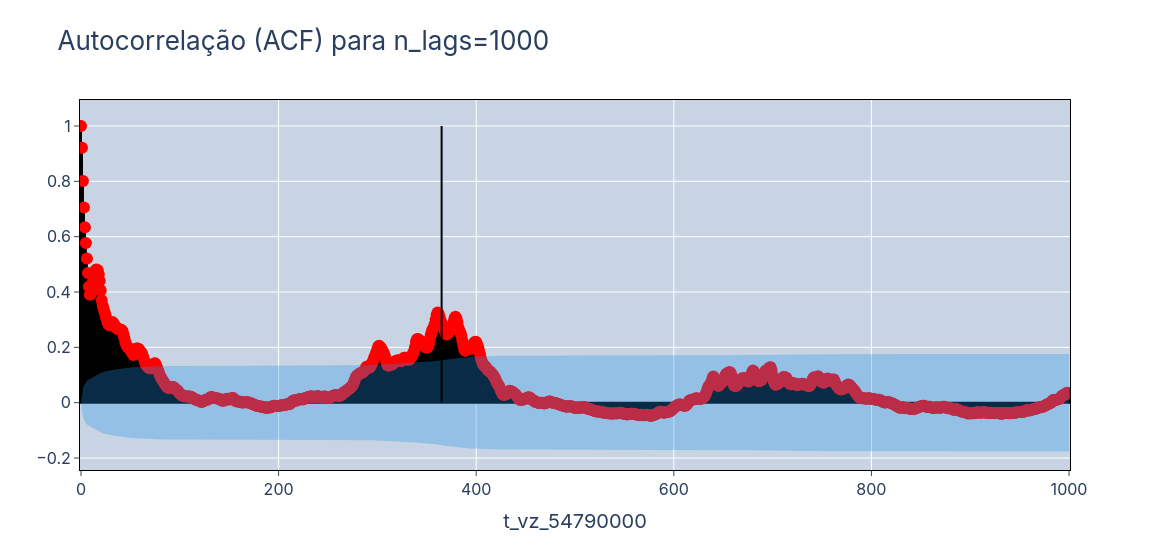
\includegraphics[scale=0.33]{Figuras/jequiti/acf_jequitinhonha.png}
	\caption{Autocorrelação para a vazão do rio Jequitinhonha\\(fonte: o autor)}
	\label{fig:acf_jequitinhonha}
\end{figure}

\begin{figure}[!h]
	\centering
	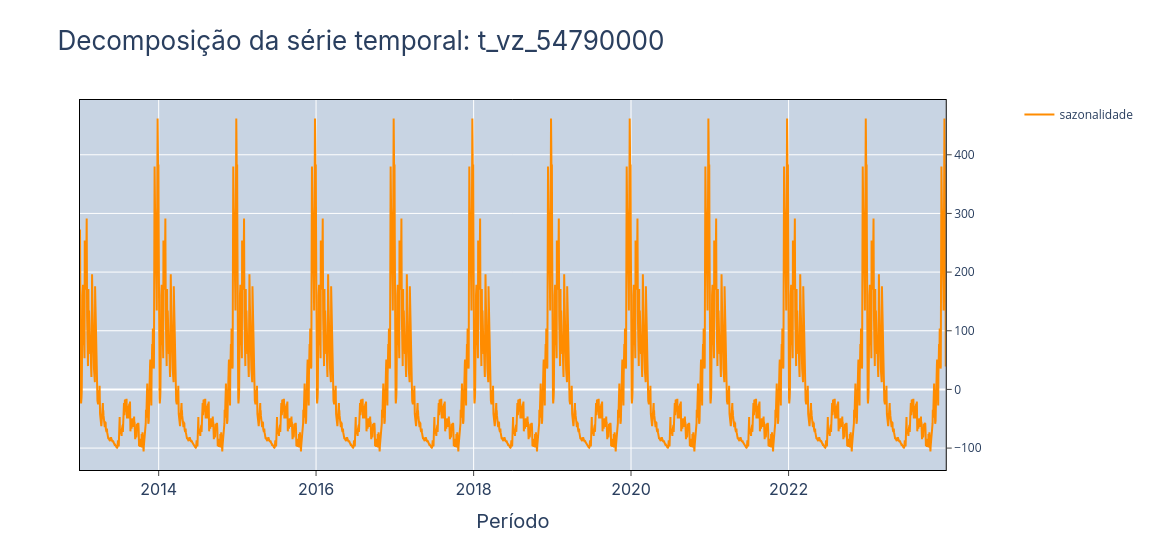
\includegraphics[scale=0.33]{Figuras/jequiti/sazonalidade_jequitinhonha.png}
	\caption{Componente sazonal da série de vazão do rio Jequitinhonha\\(fonte: o autor)}
	\label{fig:sazonalidade_jequitinhonha}
\end{figure}

\begin{figure}[!h]
	\centering
	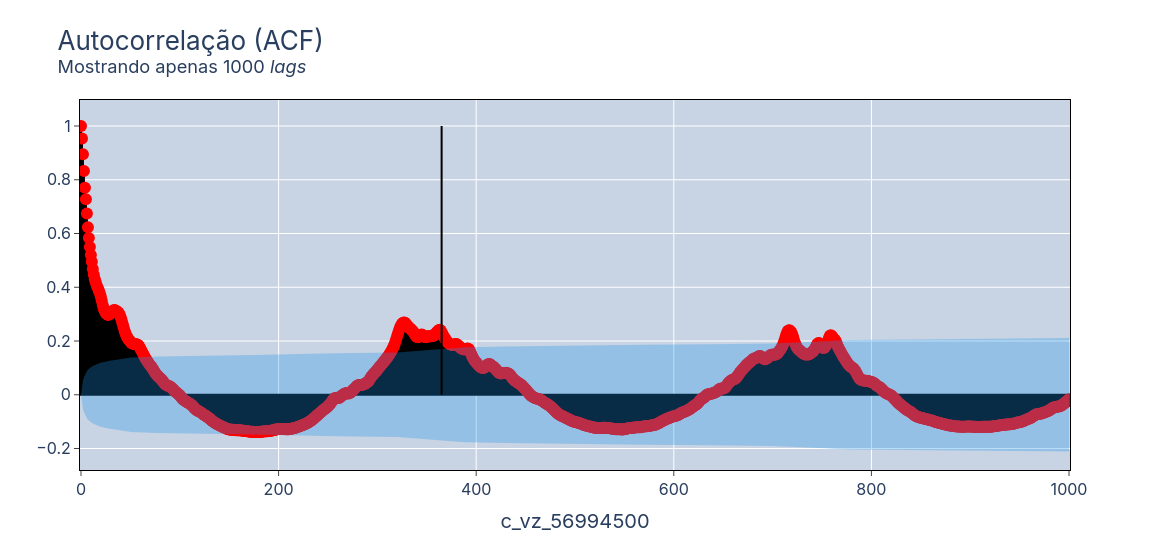
\includegraphics[scale=0.33]{Figuras/rio_doce/acf_rio_doce.png}
	\caption{Autocorrelação para a vazão do rio Doce\\(fonte: o autor)}
	\label{fig:acf_rio_doce}
\end{figure}

\begin{figure}[!h]
	\centering
	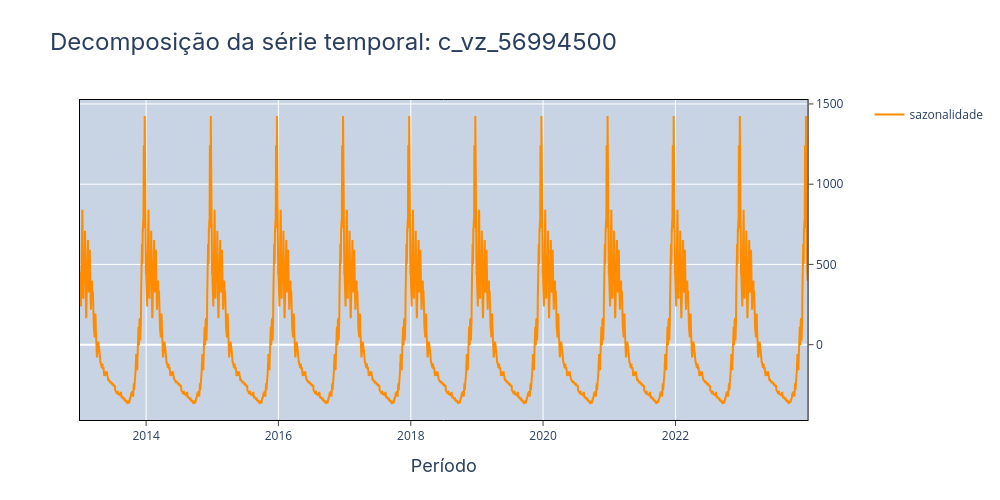
\includegraphics[scale=0.33]{Figuras/rio_doce/sazonalidade_rio_doce.png}
	\caption{Componente sazonal da série de vazão do rio Doce\\(fonte: o autor)}
	\label{fig:sazonalidade_rio_doce}
\end{figure}

\begin{figure}[!h]
	\centering
	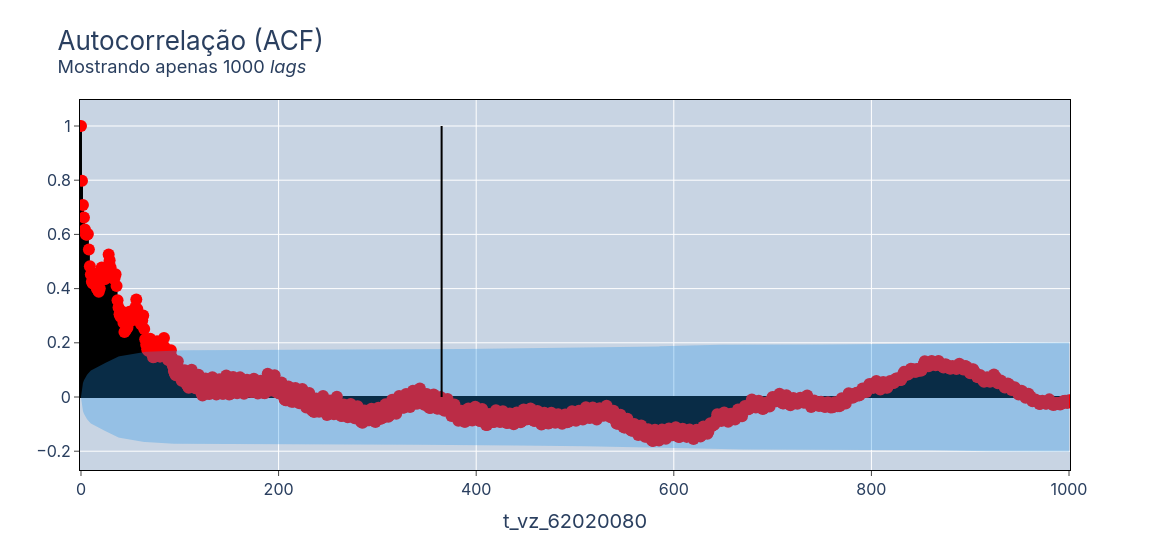
\includegraphics[scale=0.33]{Figuras/rio_grande/acf_rio_grande.png}
	\caption{Autocorrelação para a vazão do rio Grande\\(fonte: o autor)}
	\label{fig:acf_rio_grande}
\end{figure}

\begin{figure}[!h]
	\centering
	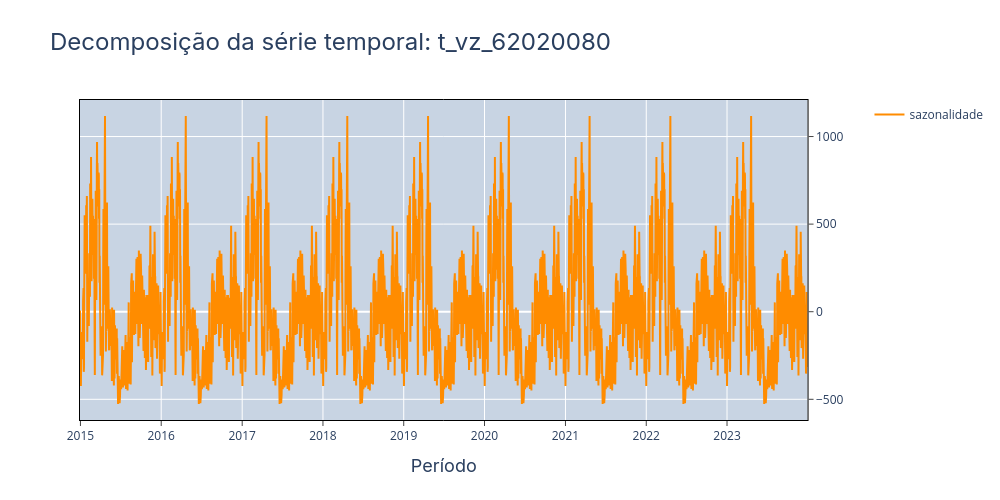
\includegraphics[scale=0.33]{Figuras/rio_grande/sazonalidade_rio_grande.png}
	\caption{Componente sazonal da série de vazão do rio Grande\\(fonte: o autor)}
	\label{fig:sazonalidade_rio_grande}
\end{figure}

\begin{figure}[!h]
	\centering
	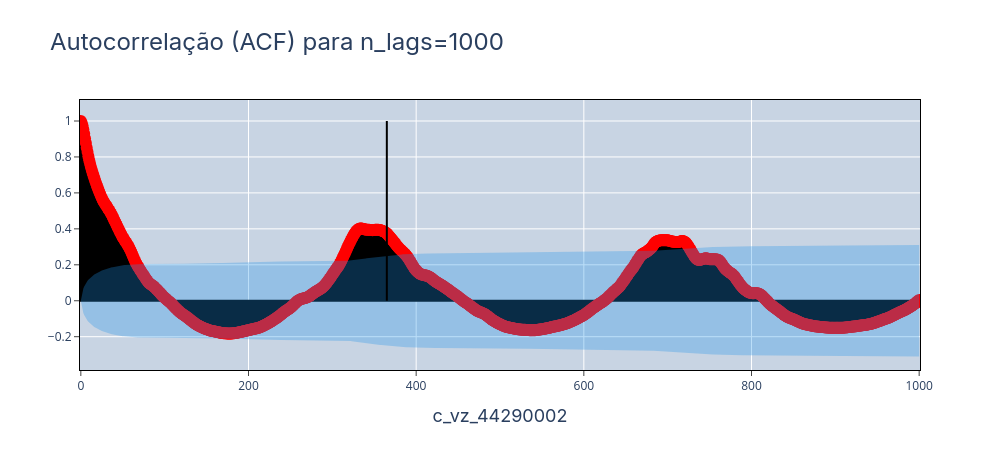
\includegraphics[scale=0.33]{Figuras/rio_sao_francisco/acf_rio_sao_francisco.png}
	\caption{Autocorrelação para a vazão do rio São Francisco\\(fonte: o autor)}
	\label{fig:acf_rio_sao_francisco}
\end{figure}

\begin{figure}[!h]
	\centering
	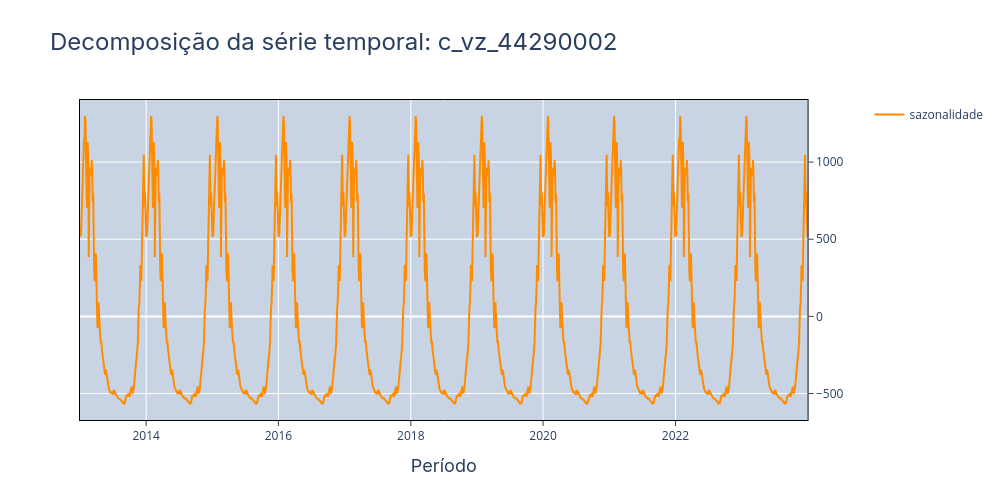
\includegraphics[scale=0.33]{Figuras/rio_sao_francisco/sazonalidade_rio_sao_francisco.png}
	\caption{Componente sazonal da série de vazão do rio São Francisco\\(fonte: o autor)}
	\label{fig:sazonalidade_rio_sao_francisco}
\end{figure}

As séries temporais consideradas, digamos, mais bem comportadas foram as dos rios Doce e São Francisco. A decomposição sazonal da série do rio Jequitinhonha apresentou algum nível de ruído, embora a sazonalidade tenha sido identificada de forma clara.

%Além da sazonalidade, a análise exploratória também incluiu a verificação da estacionariedade das séries temporais. Embora modelos estatísticos como o ARIMA não tenham sido aplicados neste trabalho, a identificação da estacionariedade é um aspecto relevante para qualquer modelo que venha a ser utilizado. Uma série estacionária possui propriedades estatísticas, como média, variância e autocorrelação, que permanecem constantes ao longo do tempo. Isso pode favorecer a convergência dos modelos preditivos e melhorar sua capacidade de previsão.
%
%Para este estudo foi aplicado um teste ADF (\textit{Augmented Dickey-Fuller} - Dickey-Fuller Aumentado) em que um valor-p (\textit{p-value}) menor ou igual a 0,05 (<= 0,05) confirmaria a estacionariedade. A biblioteca sktime tem um método pra isso e foi utilizado.\cite{loning2019sktime}

Outra característica investigada neste estudo foi a presença de `cauda longa' nos dados de precipitação e vazão. Esse comportamento é comumente observado em dados ambientais dessa natureza.\cite{elena_macdonald_2023}

A `cauda longa' refere-se a uma distribuição de frequência na qual uma proporção significativa dos eventos ocorre em uma região distante do centro ou da média da distribuição. Em uma distribuição normal, a maioria dos eventos se concentra em torno da média, com poucas ocorrências nas extremidades (caudas). No entanto, na distribuição com cauda longa, essas extremidades contêm uma quantidade substancial de eventos, que, somados, podem representar uma fração importante do total. A análise de cauda longa é um campo específico da estatística, desenvolvido para lidar com eventos de baixa frequência, mas de alta magnitude. No entanto, este trabalho não se aprofundou nas técnicas avançadas de análise de cauda longa; o foco aqui foi identificar a presença desse fenômeno e determinar um tratamento adequado para os dados.

A mitigação do efeito de cauda longa é particularmente relevante para modelos como a Regressão Linear, que pressupõe uma distribuição normal dos dados. Uma distribuição assimétrica pode comprometer a convergência do modelo. Embora os modelos baseados em \textit{boosting} utilizados neste estudo, como o CatBoost e o LightGBM, não sejam tão sensíveis a esse efeito, pois captam relações não-lineares e complexas de forma eficiente, optou-se por aplicar o mesmo tratamento a todos os modelos para garantir uma padronização na apresentação dos dados.

Dado que os dados contêm valores iguais a zero, a transformação pelo logaritmo natural (ln(.)) não foi aplicada, pois o cálculo de logaritmo não é definido para valores zero. Em vez disso, foi utilizada a transformação `log1p(.)' da biblioteca NumPy \cite{numpyref}, que adiciona 1 ao valor antes da transformação, evitando erros relacionados ao logaritmo de zero.

Após a transformação a distribuição dos eventos ficou menos assimétrica, como pode ser visto nas figuras \ref{fig:jequitinhonha_antes_log}, \ref{fig:jequitinhonha_depois_log}, \ref{fig:rio_doce_antes_log}, \ref{fig:rio_doce_depois_log}, \ref{fig:rio_grande_antes_log}, \ref{fig:rio_grande_depois_log}, \ref{fig:rio_sao_francisco_antes_log}, \ref{fig:rio_sao_francisco_depois_log}. Para o rio Grande, visualmente, parece não ter havido tanta diferença, mas quando se analisa os valores, houve um achatamento na distância entre os valores máximo e o mínimo da série.

\begin{figure}[!h]
	\centering
	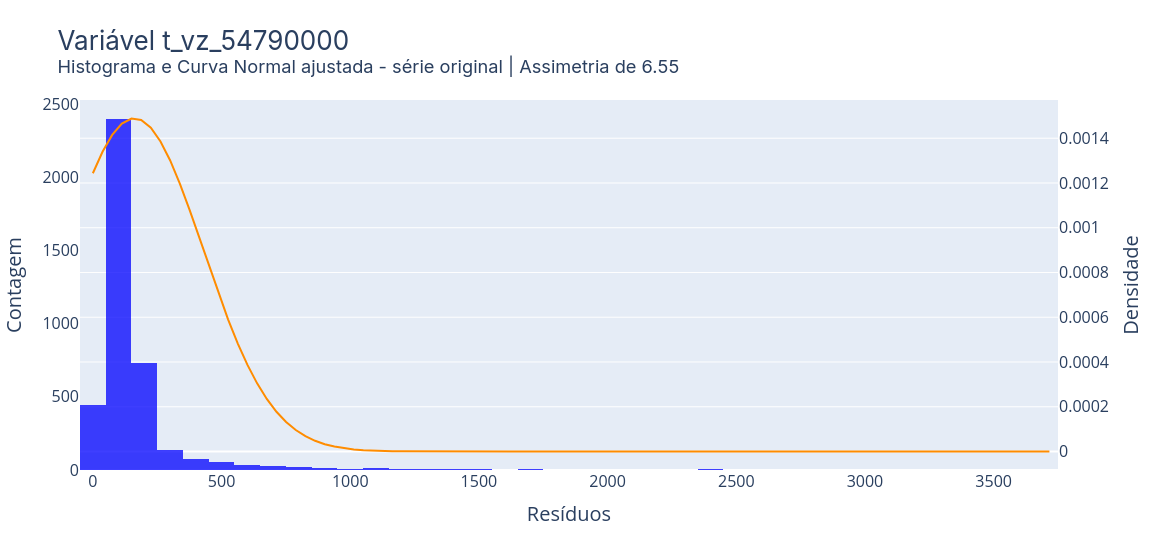
\includegraphics[scale=0.33]{Figuras/jequiti/jequitinhonha_antes_log.png}
	\caption{Dados originais para o rio Jequitinhonha\\(fonte: o autor)}
	\label{fig:jequitinhonha_antes_log}
\end{figure}

\begin{figure}[!h]
	\centering
	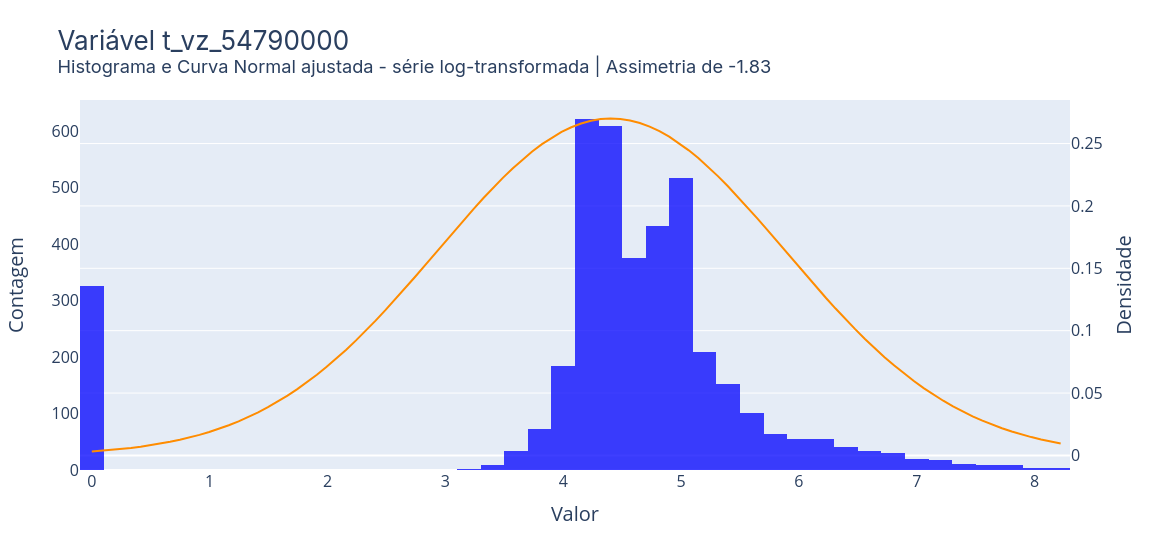
\includegraphics[scale=0.33]{Figuras/jequiti/jequitinhonha_depois_log.png}
	\caption{Dados transformados para o rio Jequitinhonha\\(fonte: o autor)}
	\label{fig:jequitinhonha_depois_log}
\end{figure}

\begin{figure}[!h]
	\centering
	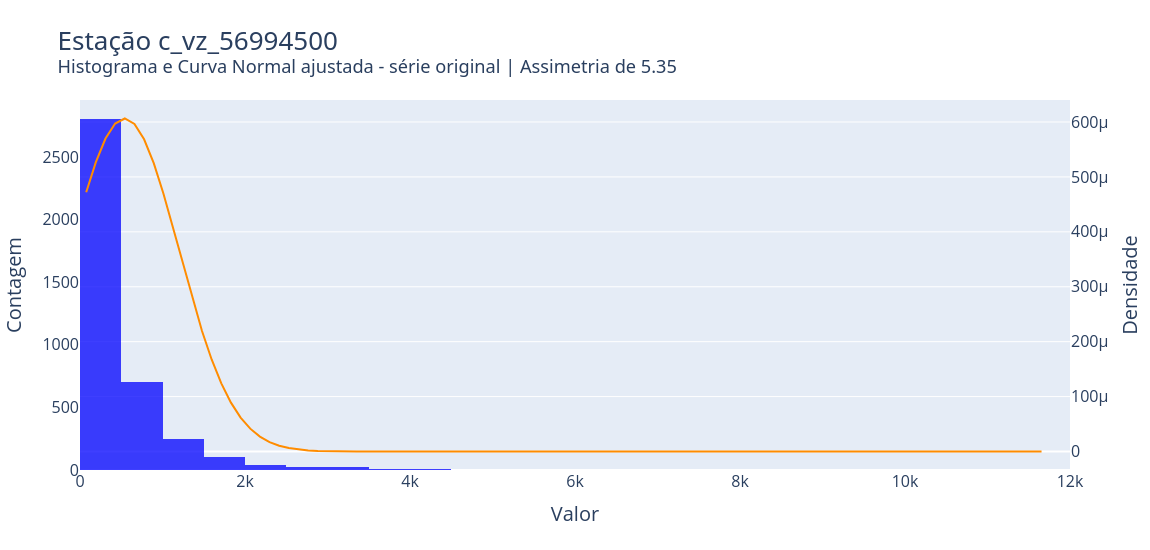
\includegraphics[scale=0.33]{Figuras/rio_doce/rio_doce_antes_log.png}
	\caption{Dados originais para o rio Doce\\(fonte: o autor)}
	\label{fig:rio_doce_antes_log}
\end{figure}

\begin{figure}[!h]
	\centering
	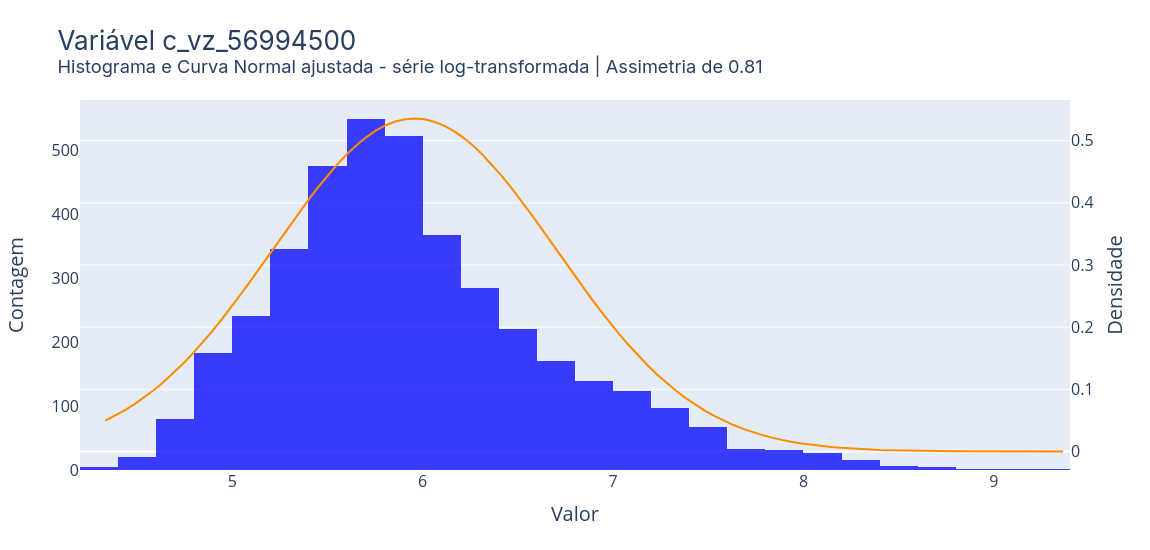
\includegraphics[scale=0.33]{Figuras/rio_doce/rio_doce_depois_log.png}
	\caption{Dados transformados para o rio Doce\\(fonte: o autor)}
	\label{fig:rio_doce_depois_log}
\end{figure}

\begin{figure}[!h]
	\centering
	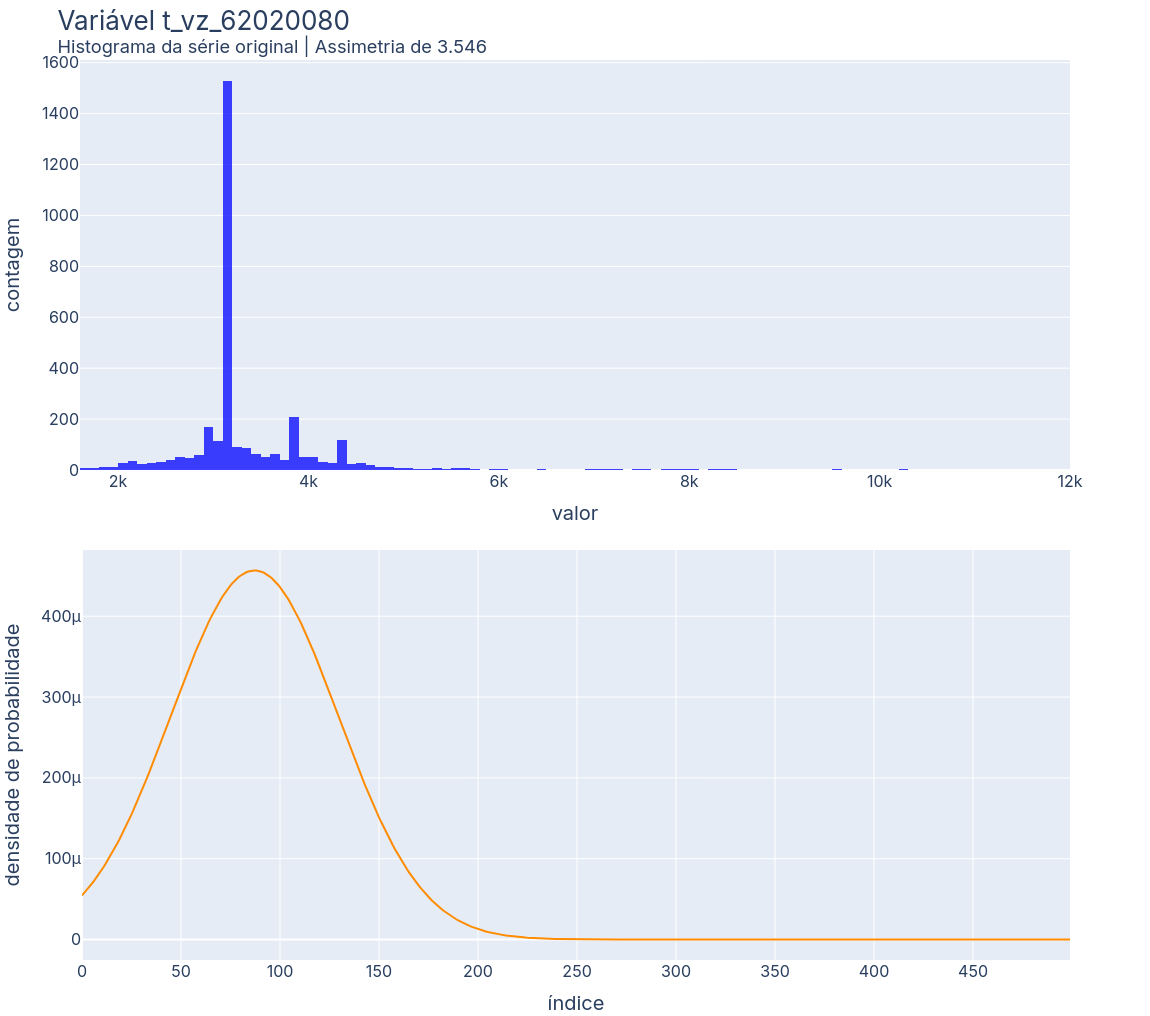
\includegraphics[scale=0.33]{Figuras/rio_grande/rio_grande_antes_log.png}
	\caption{Dados originais para o rio Grande\\(fonte: o autor)}
	\label{fig:rio_grande_antes_log}
\end{figure}

\begin{figure}[!h]
	\centering
	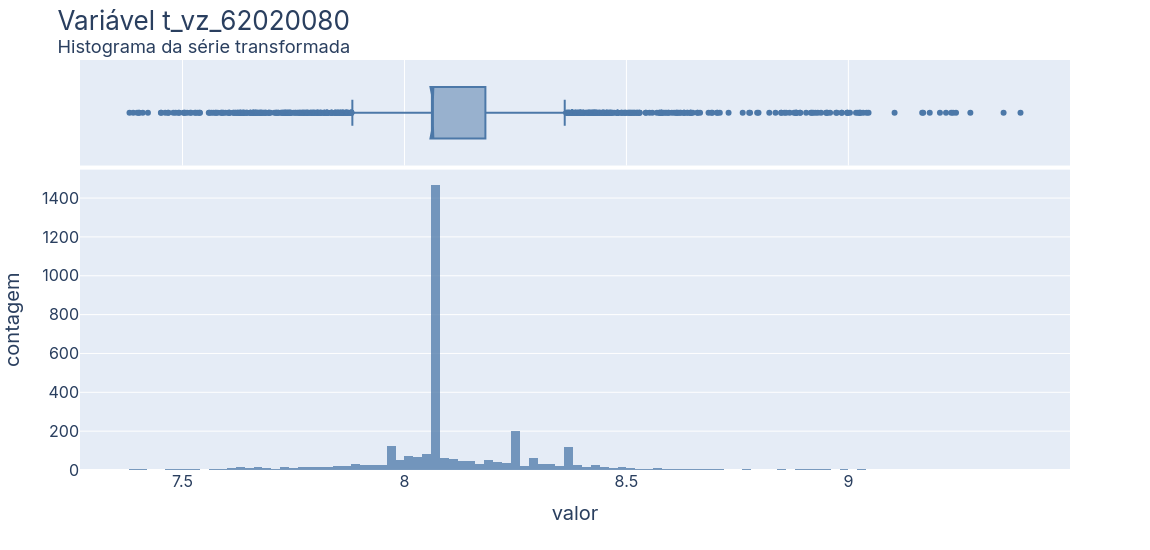
\includegraphics[scale=0.33]{Figuras/rio_grande/rio_grande_depois_log.png}
	\caption{Dados transformados para o rio Grande\\(fonte: o autor)}
	\label{fig:rio_grande_depois_log}
\end{figure}

\begin{figure}[!h]
	\centering
	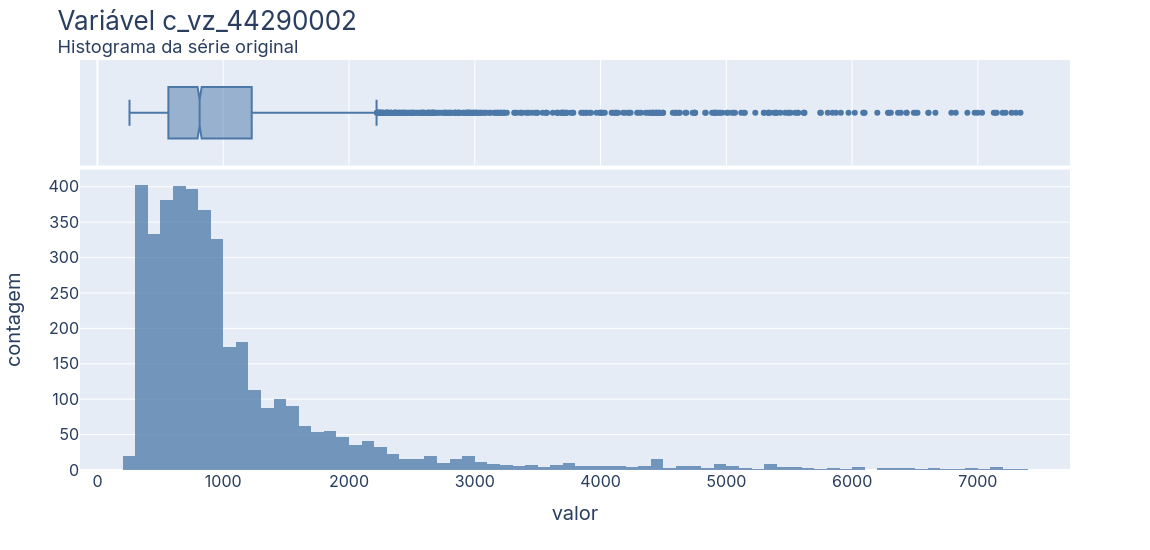
\includegraphics[scale=0.33]{Figuras/rio_sao_francisco/rio_sao_francisco_antes_log.png}
	\caption{Dados originais para o rio São Francisco\\(fonte: o autor)}
	\label{fig:rio_sao_francisco_antes_log}
\end{figure}

\begin{figure}[!h]
	\centering
	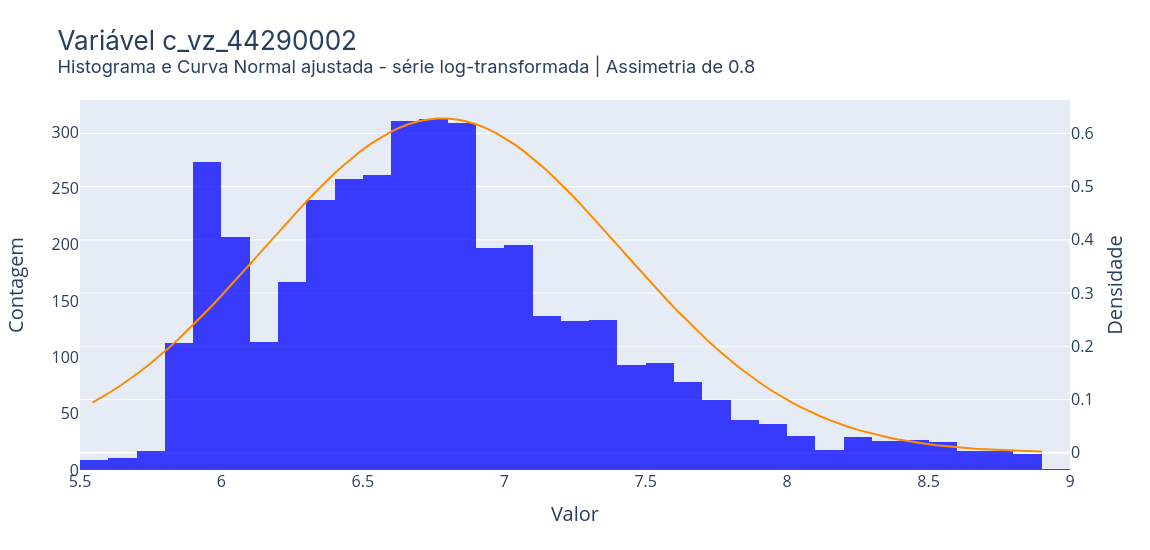
\includegraphics[scale=0.33]{Figuras/rio_sao_francisco/rio_sao_francisco_depois_log.png}
	\caption{Dados transformados para o rio São Francisco\\(fonte: o autor)}
	\label{fig:rio_sao_francisco_depois_log}
\end{figure}
\clearpage

Para finalizar, uma análise comumente realizada em séries temporais é a verificação de sua estacionariedade. No entanto, neste estudo, essa avaliação não foi realizada, pois séries temporais de dados ambientais, como precipitação e vazão, geralmente apresentam sazonalidade e tendências que violam o conceito de estacionariedade conforme explicado em \citet{hyndman_fpp3_2024e}. Outros desafios a esta análise também incluem a rápida mudança no uso do solo e remoção de cobertura vegetal original, alterando significativamente a dinâmica hidrológica da região.\cite{rayyan-33388453}

A estacionariedade pressupõe que as características estatísticas da série, como média, variância e autocorrelação, permaneçam constantes ao longo do tempo. No entanto, dados ambientais, especialmente os relacionados a fenômenos hidrológicos, costumam exibir padrões sazonais marcados e eventos extremos, o que torna inadequada a aplicação de testes de estacionariedade tradicionais. As séries de precipitação podem ser influenciadas por fatores externos, como mudanças climáticas ou eventos meteorológicos excepcionais, resultando em variações significativas ao longo do tempo. No caso da vazão, variações no uso e ocupação do solo causam impacto no escoamento.

Essas características, longe de serem consideradas como ruído ou anomalias, fazem parte da própria natureza dos dados ambientais e são cruciais para a modelagem e previsão. Assim, em vez de tentar forçar a estacionariedade, este trabalho optou por lidar com a sazonalidade e as tendências diretamente, utilizando técnicas que captam essas dinâmicas, visando garantir previsões mais realistas e representativas dos processos hidrológicos.

\section{Modelos de Aprendizado de Máquina}
%Apresentar os modelos de ML utilizados (SeasonalNaive, LinearRegression, CatBoost e LightGBM) e justificativas.

\subsection{Seasonal Naive}

O modelo \textbf{Seasonal Naive} não pode ser considerado um modelo de previsão sofisticado. Em vez disso, ele funciona como uma linha de base (baseline), servindo como ponto de partida para avaliar o desempenho de outros modelos de previsão. Este modelo simplesmente repete a sazonalidade observada no período anterior, ou seja, assume que o comportamento do próximo ciclo sazonal será o mesmo do anterior, com um possível ajuste por \textit{drift} (desvio).\cite{hyndman_fpp3_2024d}

Esse método é útil para fornecer uma idéia inicial do comportamento esperado, permitindo que os modelos subsequentes sejam comparados a ele. Por ser um modelo simples, ele não captura tendências ou variações complexas, mas estabelece um \textit{benchmark} mínimo para o qual outros métodos mais elaborados e complexos devem se comparar.

\subsection{Regressão Linear}

O modelo de Regressão Linear (\textit{Linear Regression}) é uma abordagem estatística simples, porém poderosa, que busca modelar o relacionamento entre uma variável dependente e uma ou mais variáveis independentes através de uma linha reta. 

O funcionamento da Regressão Linear envolve o cálculo de coeficientes para as variáveis independentes, que determinam o peso de cada uma destas variáveis na previsão da variável dependente. O objetivo do modelo é minimizar o erro quadrático médio, ou seja, a soma dos quadrados das diferenças entre os valores previstos e os valores reais.\cite{hyndman_fpp3_2024c}

Os resultados obtidos com este modelo mostraram-se muito bons, e na verdade, ele se destacou como um modelo-base robusto para os outros modelos mais complexos. Sua simplicidade e eficácia tornam-no uma escolha bastante sólida. Isso será discutido.

% Aqui está o fluxograma para o funcionamento do modelo de Regressão Linear \todo[inline]{INSERIR DIAGRAMA ?}

\subsection{CatBoost e LightGBM}

Estes dois modelos são descritos juntos pois o funcionamento de ambos se baseia no mesmo princípio: ambos algoritmos constroem modelos fracos de árvores de decisão (\textit{decision tree}) de forma sequencial, onde cada árvore sucessiva é treinada para corrigir os erros da árvore anterior. Contudo, o LightGBM adota uma estratégia denominada ``Leaf-wise Growth'' ao invés da forma de construção tradicional ``Level-wise Growth''. Nesta estratégia, o crescimento ocorre folha a folha, a árvore expande as folhas com a maior redução de erro, resultando em árvores mais profundas e precisas.\cite{ke2017lightgbm}\cite{LightGBM} O revés nessa estretégia é que fica mais suscetível a \textit{overfitting}, mas existem parâmetros no modelo, como por exemplo `min\_data\_in\_leaf' (quantidade mínima de dados em cada folha) que cuidam para que isso seja evitado.

O CatBoost, por sua vez, adota uma estratégia denominada ``Ordered Boosting'', em que a construção das árvores se dá de maneira sequencial, porém não se usa todos os dados disponíveis para esta construção. Os dados de treinamento são ordenados de maneira aleatória e apenas partições destes dados são utilizados no processo. Por trabalhar sempre com uma amostra dos dados de treinamento, e a apresentação aleatória destes dados ao modelos, o CatBoost tem resiliência ao \textit{overfitting}, mas parâmetros que realizam ajustes nas árvores de decisão também estão presentes e o pesquisador tem controle sobre eles.\cite{catboost_docs}\cite{dorogush2018catboost}\cite{prokhorenkova2018catboost}

%\begin{figure}[!h]
%	\centering
%	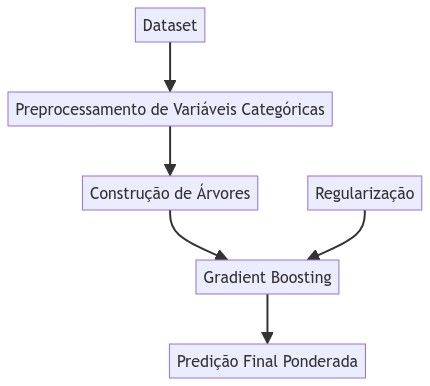
\includegraphics[scale=0.75]{Figuras/boosting_diagrama.jpg}
%	\caption{Diagrama resumindo o funcionamento dos modelos de \textit{boosting} (fonte: o autor)}
%	\label{fig:boosting_diagrama}
%\end{figure}

A escolha do modelo certo para um problema de previsão desta natureza depende das características dos dados e dos objetivos do estudo. O SeasonalNaive, embora simples, é um importante ponto de referência inicial. O modelo de Regressão Linear serve como uma \textit{baseline} confiável devido à sua eficácia e simplicidade. Já os modelos CatBoost e LightGBM foram opções mais avançadas, capazes de lidar com a complexidade dos dados e oferecer previsões precisas e eficientes. A comparação entre todos estes modelos permitiu que se escolhesse a abordagem que melhor atendesse às necessidades específicas da previsão de vazões.

\section{Métricas de Avaliação}
%Listar as métricas usadas para avaliar o desempenho dos modelos (MAPE, RMSE, PBias* e KGE não-paramétrico**).
%(*: PBias ajuda a ver se o modelo está subestimando as previsões ou superestimando)
%(**: KGEnp (não paramétrico) é uma métrica comum e muito consagrada na hidrologia. Ela tem resiliência a outliers ao avaliar a qualidade do modelo)

Para avaliar o desempenho dos modelos de previsão utilizados neste estudo, foram adotadas quatro métricas: MAPE (\textit{Mean Absolute Percentage Error}), RMSE (\textit{Root Mean Square Error}), PBIAS (\textit{Percent Bias}) e KGE (\textit{Kling-Gupta Efficiency}). A escolha dessas métricas baseia-se na necessidade de uma avaliação abrangente que considere diferentes aspectos da qualidade das previsões, como precisão, erro médio, tendência e correlação.

\begin{itemize}
	\item \textbf{MAPE (\textit{Mean Absolute Percentage Error})}: O MAPE é uma métrica amplamente utilizada para medir a precisão das previsões em termos percentuais. O algoritmo calcula a média das diferenças absolutas entre os valores observados e previstos, normalizadas pelos valores observados. O bom da métrica MAPE é a sua facilidade de interpretação, já que expressa o erro em termos percentuais, e por ser ``livre de escala'', ou seja, independente da escala dos dados, tornando os resultados comparáveis entre diferentes séries temporais e modelos. Contudo, o MAPE pode ser sensível a valores muito baixos e esta característica deve ser considerada ao interpretar os resultados. Quanto mais próximo de 0, melhor.\cite{hyndman_fpp3_2024b}
	\begin{equation}
		MAPE = \frac{100}{n} \sum_{i=1}^{n} \left| \frac{O_i - P_i}{O_i} \right|
	\end{equation}
	\begin{itemize}
		\item $O_i$ valores observados
		\item $P_i$ valores previstos
		\item $n$ o número total de observações
	\end{itemize}
	
	\item \textbf{RMSE (\textit{Root Mean Square Error})}: O RMSE mede o erro médio das previsões, penalizando erros maiores devido à sua formulação quadrática. Essa métrica é amplamente utilizada por sua sensibilidade a grandes desvios entre as previsões e os valores observados, o que a torna adequada para identificar erros extremos. O RMSE é uma escolha natural quando se deseja minimizar grandes erros e garantir maior precisão nas previsões. Quanto menor, melhor.\cite{hyndman_fpp3_2024b}
	\begin{equation}
		RMSE = \sqrt{\frac{1}{n} \sum_{i=1}^{n} (P_i - O_i)^2}
	\end{equation}
	\begin{itemize}
		\item $O_i$ valores observados
		\item $P_i$ valores previstos
		\item $n$ o número total de observações
	\end{itemize}

	\item \textbf{$R^2$ (\textit{Coefficient of Determination})}: O Coeficiente de Determinação, que é o quadrado do coeficiente de correlação de Pearson, mede a proporção da variância total nos dados observados que pode ser explicada pelo modelo. Ele varia de 0,0 a 1,0, com valores mais alto indicando uma melhor concordância entre os dados observados e os previstos. Embora o $R^2$ seja amplamente utilizado, ele apresenta limitações que podem resultar em uma avaliação imprecisa do desempenho de modelos hidrológicos, tal como ser uma métrica sensível a valores discrepantes (\textit{outliers}) e avaliar apenas relações lineares. Deve ser empregado com outras métricas para garantir uma boa interpretabilidade dos resultados dos modelos.\cite{legates1999goodness}
	\begin{equation}
		R^2 = 1 - \frac{\sum_{i=1}^{n} (O_i - {P_i})^2}{\sum_{i=1}^{n} (O_i - \bar{O})^2}
	\end{equation}
	\begin{itemize}
		\item $O_i$ valores observados
		\item $P_i$ valores previstos
		\item $\bar{O}$ média dos valores observados
		\item $n$ o número total de observações
	\end{itemize}
	
	\item \textbf{PBIAS (\textit{Percent Bias})}: O PBIAS avalia o viés das previsões, ou seja, a tendência do modelo em superestimar (PBIAS positivo) ou subestimar (PBIAS negativo) os valores observados. Ele expressa a diferença percentual entre a soma dos valores previstos e observados, permitindo identificar se o modelo apresenta uma tendência sistemática de erro. Um valor de PBIAS próximo de zero indica que o modelo não possui viés significativo. Não se espera que esta métrica seja 0, senão indicaria que a previsão foi exatamente o valor observado, mas ao mostrar o viés das previsões, isso tem impacto diretamente nas decisões de gestão de recursos hídricos.\cite{rayyan-33388455}
	\begin{equation}
		PBIAS = 100 \times \frac{\sum_{i=1}^{n} (P_i - O_i)}{\sum_{i=1}^{n} O_i}
	\end{equation}
	\begin{itemize}
		\item $O_i$ valores observados
		\item $P_i$ valores previstos
		\item $n$ o número total de observações
	\end{itemize}
	
	\item \textbf{KGE (\textit{Kling-Gupta Efficiency})}: O KGE fornece uma avaliação integrada do desempenho do modelo, considerando simultaneamente três componentes: correlação, viés e variabilidade relativa entre os valores previstos e observados. O KGE é uma métrica robusta que combina esses três fatores de forma equilibrada, fornecendo um entendimento geral da qualidade das previsões. Essa métrica é especialmente útil em estudos hidrológicos, pois tem capacidade de capturar a complexidade das relações entre variáveis hidrológicas de maneira mais eficaz do que métricas tradicionais focadas em um único aspecto. Quanto mais próximo de 1, melhor o desempenho do modelo.\cite{Gupta2009}
	
	\begin{equation}
		KGE = 1 - \sqrt{(r - 1)^2 + (\alpha - 1)^2 + (\beta - 1)^2}
	\end{equation}
	\begin{itemize}
		\item $r$ é o coeficiente de correlação linear entre os valores observados e previstos 
		\item $\alpha = \frac{\sigma_p}{\sigma_o}$ é a variabilidade relativa, sendo $\sigma_p$ o desvio-padrão das previsões e $\sigma_o$ o desvio-padrão das observações
		\item $\beta = \frac{\mu_p}{\mu_o}$ é o viés, em que $\mu_p$ é a média dos valores previstos e $\mu_o$ a média dos valores observados		
	\end{itemize}
	
\end{itemize}

%\section{Treinamento e Validação dos Modelos}
%Detalhar os procedimentos de treinamento e validação dos modelos.

\section{Modelo proposto}
% Detalhar os procedimentos de treinamento e validação dos modelos.

Tudo detalhado até aqui, agora é preciso descrever o fluxo de trabalho. Por fim, será apresentado o fluxograma do modelo proposto para uma rápida depreensão visual.

Primeiramente é necessário especificar o período histórico de análise. Depois de estipulado o período, deve-se identificar as estações de vazão para as quais serão realizadas as previsões.

Identificadas estas estações de vazão, verifica-se em linha reta, em sentido montante da estação de vazão, as estações de precipitação a 50km nas sub-bacias que deságuam no corpo hídrico analisado. Para este passo foi utilizado o programa QGis com \textit{shapefiles} das ottobacias.\cite{snirh_ottobacia_2024} Para o \textit{shapefile} de todas as estações do estado de Minas Gerais foi preciso acesso ao sistema da empresa Rhama Analysis. Sistema fechado este, no caso.

%{\color{red}No passo de verificação dos dados faltantes, o preenchimento foi realizado aplicando a média dos últimos 3 anos para os dias faltantes. O que ainda restou faltando, um modelo kNN finalizou o preenchimento usando os 7 vizinhos mais próximos.} \todo[inline, color = blue, textcolor=white]{já foi dito}

Aqui uma importante etapa: aplicar transformação logarítmica nos dados de vazão e precipitação para tratar o fenômeno de ``cauda'' longa dos dados.

A separação dos dados do último ano, 2023, foi para posteriormente simular o uso dos modelos ao longo de um ano. Realizar ajuste (`\textit{fit}') e previsão (`predict'), dia-a-dia, durante um ano inteiro, para avaliar a estabilidade dos modelos. Este procedimento é referido na literatura como \textit{Walk-Forward Validation} (WFV) e pode ser por uma janela deslizante ou por janela expandida, que foi a técnica aplicada neste trabalho. Além disso, tem duas formas de realizar as previsões: criando vários modelos que irão prever cada um dos dias futuros (`direct forecasting'), o que geraria 365 modelos distintos e, consequentemente, consumiria muita mémoria, ou o que foi adotado neste trabalho que foi realizar reajustes (`\textit{refit}') ao modelo inicial num processo recursivo (`recursive forecasting'). Esse processo de WFV permite capturar mudanças ao longo do tempo e avaliar a capacidade do modelo de generalizar para o futuro de forma mais realista. Perceba o funcionamento nas imagens a seguir (observação: a fonte de onde as imagens foram retiradas nomeia o processo de Walk-Forward Validation como `backtesting' \cite{skforecast})

\begin{figure}[!h]
	\centering
	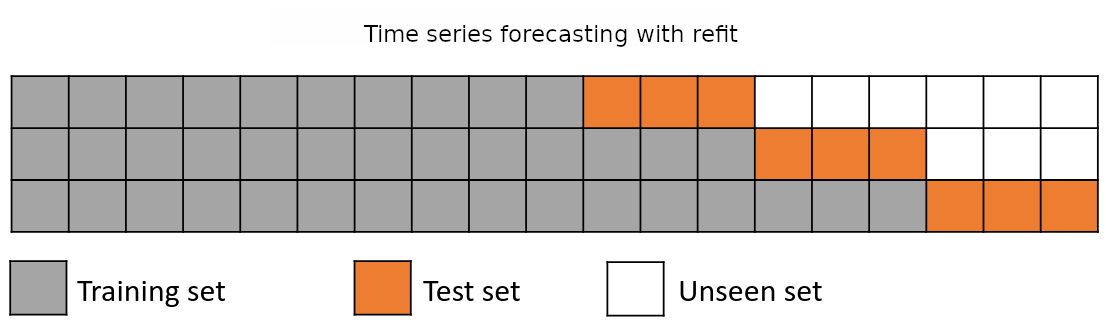
\includegraphics[scale=0.3]{Figuras/skforecast-diagram-backtesting-refit.png}
	\caption{Diagrama mostrando a divisão dos dados de treino/teste com \textit{refit}.\\(fonte: \cite{skforecast})}
	\label{fig:skforecast-diagram-backtesting-refit}
\end{figure}

\begin{figure}[!h]
	\centering
	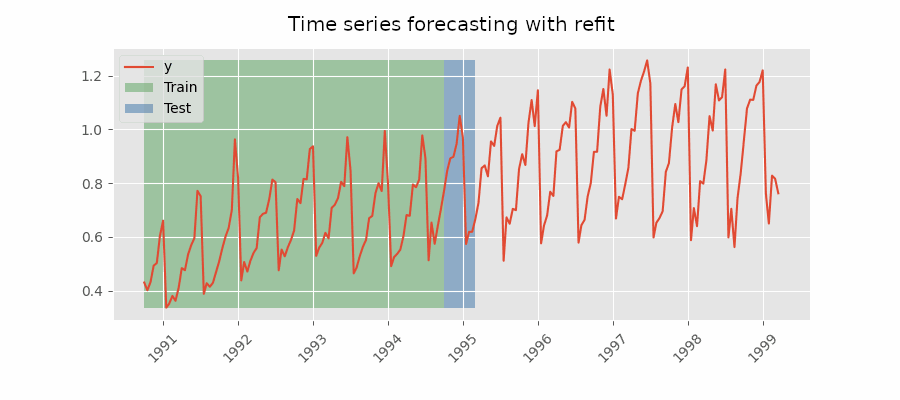
\includegraphics[scale=0.3]{Figuras/imagem1_skforecast-backtesting-refit.png}
	\caption{WFV com janela expandida e \textit{refit} - imagem 1.\\(fonte: \cite{skforecast})}
	\label{fig:imagem1_skforecast-backtesting-refit}
\end{figure}

\begin{figure}[!h]
	\centering
	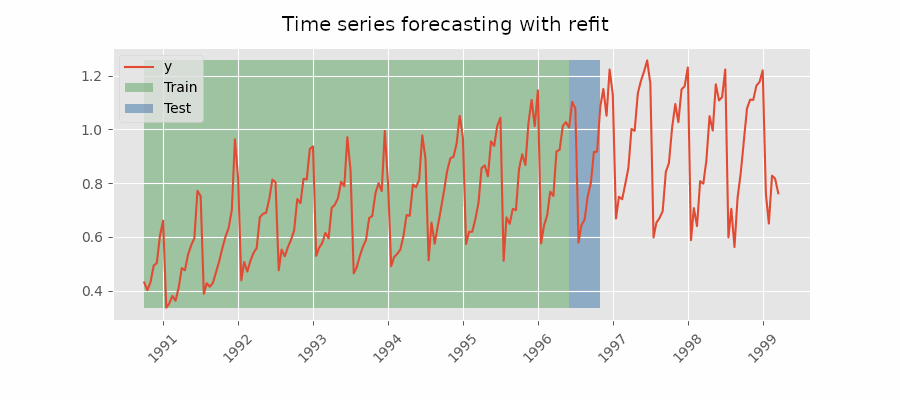
\includegraphics[scale=0.3]{Figuras/imagem2_skforecast-backtesting-refit.png}
	\caption{WFV com janela expandida e \textit{refit} - imagem 2.\\(fonte: \cite{skforecast})}
	\label{fig:imagem2_skforecast-backtesting-refit}
\end{figure}

\begin{figure}[!h]
	\centering
	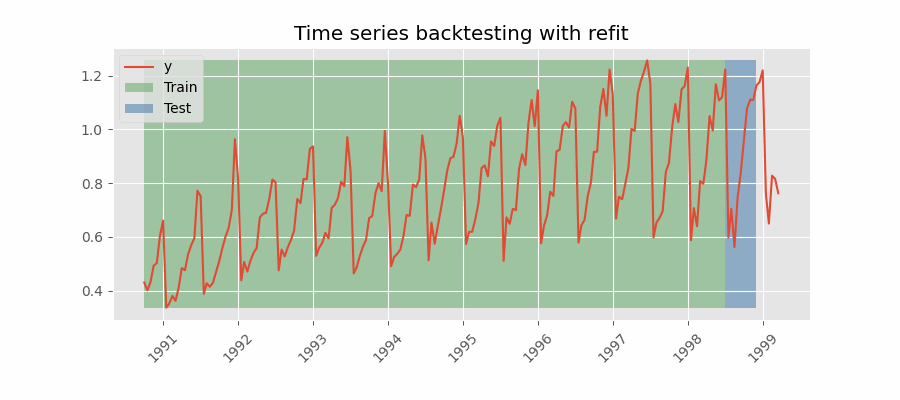
\includegraphics[scale=0.3]{Figuras/imagem3_skforecast-backtesting-refit.png}
	\caption{WFV com janela expandida e \textit{refit} - imagem 3.\\(fonte: \cite{skforecast})}
	\label{fig:imagem3_skforecast-backtesting-refit}
\end{figure}

Com os dados restantes, a saber, de 2013 a 2022, foram realizadas avaliações em alguns horizontes de previsão antes de partir para a análise mais complexa (WFV). A intenção era compreender o comportamento da modelagem em horizontes curtos e médios. Foram escolhidos os horizontes de previsão de 1, 3, 7 e 15 dias. As previsões utilizaram a previsão multietapas, com modelos diretos, ou seja, após feito o ajuste, cada dia foi previsto reiteradamente sem reajuste dos pesos e parâmetros internos dos modelos (``direct forecast''). Veja a seguir o procedimento.

\begin{figure}[!h]
	\centering
	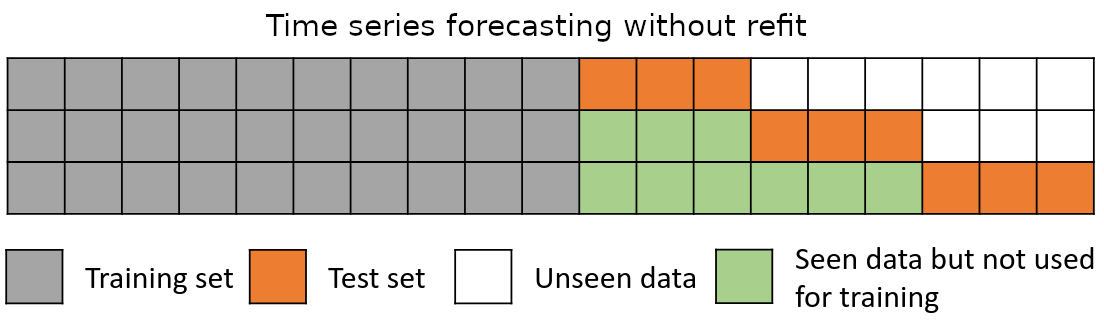
\includegraphics[scale=0.3]{Figuras/skforecast-diagram-backtesting-no-refit.png}
	\caption{Diagrama mostrando a divisão dos dados de treino/teste sem \textit{refit}.\\(fonte: \cite{skforecast})}
	\label{fig:skforecast-diagram-backtesting-no-refit}
\end{figure}

\begin{figure}[!h]
	\centering
	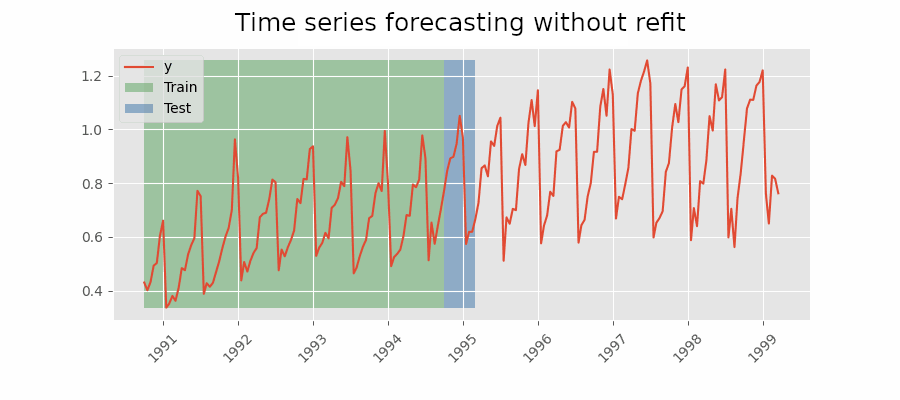
\includegraphics[scale=0.3]{Figuras/imagem1_skforecast-backtesting-no-refit.png}
	\caption{Previsão multietapas sem reajuste (\textit{refit}) - imagem 1.\\(fonte: \cite{skforecast})}
	\label{fig:imagem1_skforecast-backtesting-no-refit}
\end{figure}

\begin{figure}[!h]
	\centering
	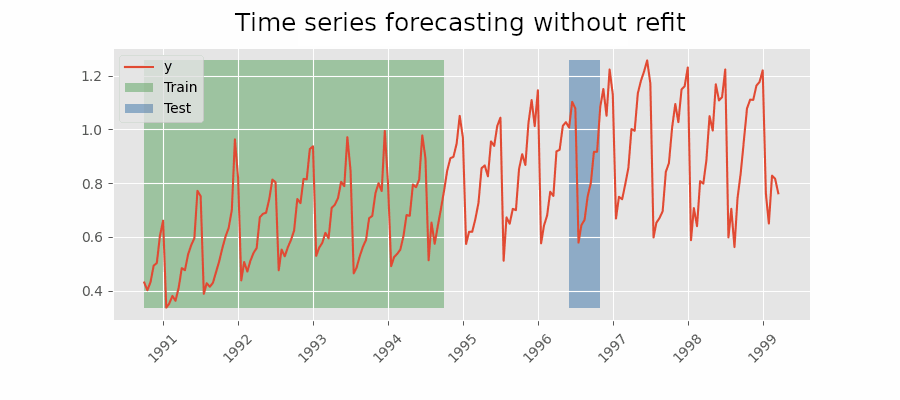
\includegraphics[scale=0.3]{Figuras/imagem2_skforecast-backtesting-no-refit.png}
	\caption{Previsão multietapas sem reajuste (\textit{refit}) - imagem 2.\\(fonte: \cite{skforecast})}
	\label{fig:imagem2_skforecast-backtesting-no-refit}
\end{figure}

\begin{figure}[!h]
	\centering
	\includegraphics[scale=0.3]{Figuras/imagem3_skforecast-backtesting-no-refit.png}
	\caption{Previsão multietapas sem reajuste (\textit{refit}) - imagem 3.\\(fonte: \cite{skforecast})}
	\label{fig:imagem3_skforecast-backtesting-no-refit}
\end{figure}

Evidentemente que para o horizonte de previsão de 1 dia não há reexecução do modelo, apenas para os outros horizontes.

O desempenho dos resultados são avaliados com as métricas propostas, para cada modelo do trablaho e para cada horizonte de previsão. Para cada horizonte de previsão foram calculados intervalos de previsão (``\textit{prediction intervals}'') de 90\%. A interpretação do intervalo de previsão é: calculados os valores inferior e superior do intervelo de 90\% (``\textit{lo-90}'' e ``\textit{hi-90}''), o valor real observado futuro tem 90\% de probabilidade de estar dentro destes limites.\cite{hyndman_fpp3_2024a}

Estes resultados encerram a análise para o comportamento de curto e médio prazo da modelagem proposta para os modelos propostos. Na sequência foi empreendida uma análise quanto à forma de uso que este trabalho pode vir a ter na prática, que é a Walk-Forward Validation. E finalmente, análise das variáveis do trabalho, buscando entendimento quanto à importância desemepenhada por cada uma, empregando o método SHAP.

%Antes, porém, foi realizada uma busca de hiperpâmetros nos modelos LightGBM e CatBoost. A busca de hiperparâmetros visa otimizar o desempenho dos modelos ao encontrar a melhor combinação de hiperparâmetros, adequadamente ajustados aos dados. Este processo foi realizado utilizando o \textit{framework} Optuna e validação-cruzada dividindo os dados de 10 anos (2013 a 2022) em 10 segmentos (\textit{folds}).\cite{akiba2019optuna}\cite{optuna_docs}\cite{skforecast}

%Com os melhores hiperparâmetros encontrados, aí sim procedeu-se para a última etapa da análise: aplicar Walk-Forward Validation.

Os resultados serão apresentados no \hyperref[cap:capitulo4]{capítulo 4}.
\clearpage

\todo[inline]{REFAZER O FLUXOGRAMA}

\begin{figure}[!h]
	\centering
	\includegraphics[scale=0.4]{Figuras/flowchart.png}
	\caption{Fluxo de trabalho\\(fonte: o autor)}
	\label{fig:fluxo_trabalho}
\end{figure}
\chapter{RESULTADOS E DISCUSS\~AO}
\label{cap:capitulo4}

\section{Desempenho dos modelos}
%Apresentar e comparar os resultados dos diferentes modelos utilizados.

Os resultados obtidos pelos modelos apresentaram variações significativas em termos de precisão, tanto nas previsões pontuais quanto nos intervalos de confiança, refletindo diferentes graus de precisão para cada cenário analisado. A análise dos resíduos revelou-se particularmente interessante, pois evidenciou comportamentos distintos em função da sazonalidade, com variações marcantes observadas em diferentes períodos do ano.

\subsection{Rio Jequitinhonha}

Iniciando pela menor bacia hidrográfica estudada, os resultados revelaram-se bastante satisfatórios, especialmente no que se refere ao modelo de Regressão Linear, que se destacou com previsões precisas, tanto em termos pontuais quanto nos intervalos de confiança. Este modelo demonstrou uma capacidade robusta de capturar a dinâmica hidrológica do rio, refletindo precisão nas métricas e desempenho consistente, aliado a um tempo de execução significativamente reduzido. Em contrapartida, o modelo (simples) SeasonalNaive apresentou resultados abaixo das expectativas em todas as situações avaliadas. (figura \ref{fig:jequiti_SN_WFV})

Com a MAPE extremamente elevada, de 150\%, os resultados indicaram um viés significativo de superestimação, conforme evidenciado pela métrica PBIAS. Verificando a KGE, ficou negativa. Em outras palavras, isso significa que o modelo não apenas falha em capturar a variabilidade dos dados observados, mas também introduz erros que o tornam menos eficaz do que uma abordagem simplista, como utiilizar a média histórica. Embora a análise superficial da qualidade dos intervalos de confiança pudesse sugerir um desempenho satisfatório do modelo, uma inspeção mais detalhada revela uma incongruência: os valores inferiores do intervalo (lo-95) foram calculados abaixo de zero, o que não faz sentido para o rio em questão, pois implicaria na ausência total de vazão, algo inviável para as condições medidas pela estação. Além disso, o atraso (\textit{delay}) da série prevista foi considerável, atingindo 56,88 dias, com um desvio-padrão de 61,3 dias, sugerindo que um evento pode demorar mais de 60 dias para ser refletido na previsão do modelo.

Considerando o desempenho insatisfatório do modelo SN, a análise foi encerrada neste ponto, sem proceder com a avaliação dos resíduos ou a análise da importância das variáveis. O modelo foi incluído apenas para fins comparativos. A análise mais aprofundada será dedicada aos modelos mais complexos, que apresentaram desempenho superior.

\begin{figure}[!h]
	\centering
	\includegraphics[scale=0.33]{Figuras/jequiti/resultados/SN_WFV.png}
	\caption{Resultado do SeasonalNaive no teste \textit{Walk-Forward Validation}\\(fonte: o autor)}
	\label{fig:jequiti_SN_WFV}
\end{figure}

%\begin{table}[!h]
%	\centering \small
%	\caption{Resultados SeasonalNaive - rio Jequitinhonha \\(fonte: o autor)}
%	\begin{tabular}{|l|r|r|r|r|r|r|} \hline 
	%		\textbf{Horizonte} & \textbf{MAPE} & \textbf{RMSE} & \textbf{PBIAS} \\\hline
	%		1 dia              & 0,871         & 831,44        & -87,11 \\\hline
	%		3 dias             & 1,528         & 1872,25       & 102,71 \\\hline
	%		7 dias             & 1,046         & 1529,13       & 49,64  \\\hline
	%		15 dias            & 0,791         & 1468,02       & -13,46 \\\hline
	%	\end{tabular}
%	\label{tab:sn_jequitinhonha_resultados}
%\end{table}

Os resultados obtidos utilizando o modelo de Regressão Linear mostraram-se bastante promissores.(figura \ref{fig:jequiti_LR_WFV_LOG}) Nesta primeira avaliação, os dados foram log-transformados. Isso é verificável pelo título com o uso de ``destransformados''. Os dados foram log-transformados e retornados para a escala original para desenhar o gráfico e ficarem acessíveis para quem lê. \underline{Essa dinâmica no título se manterá por todo trabalho}.

Partindo pela KGE calculada, o resultado mostrou-se excelente. Recordando: quanto mais próxima de 1, melhor. Este valor sugere que o modelo é eficaz na previsão do comportamento hidrológico do sistema em análise, oferecendo previsões que estão bem alinhadas com os dados observados. A MAPE de 14\% sugere que o modelo tem uma precisão razoável e é bastante confiável. O modelo apresentou um viés sistemático de subestimar os resultados, conforme aponta a PBIAS de -1,76\%. Considerando todas as métricas, o resultado indica que o modelo teve um desempenho global muito bom. A KGE alta é particularmente indicativa de um bom ajuste global, com o modelo capturando bem tanto a dinâmica quanto a magnitude dos dados observados.

Considerando a qualidade dos intervalos de previsão, a cobertura observada de 97,81\% excedeu o intervalo teórico calculado de 95\%, o que, à primeira vista, poderia ser interpretado como um desempenho satisfatório. No entanto, o limite superior do intervalo (hi-95) mostrou-se excessivamente elevado nos meses de janeiro e fevereiro, o que pode comprometer a interpretação dos resultados. Isso ocorre porque intervalos de previsão excessivamente amplos podem capturar praticamente qualquer valor observado, reduzindo a utilidade prática da previsão.

É importante destacar que os intervalos de previsão são calculados a partir dos erros do modelo durante a etapa de treinamento (\textit{in-sample residuals}). Para uma análise mais aprofundada desse comportamento, é necessário examinar os dados anteriores a 2023. A figura \ref{fig:jequiti_LR_final_2022_detalhe} revela que, nos últimos dias de 2022, houve observações significativamente elevadas. É provável que os erros associados a esse período mais próximo tenham influenciado a amplitude dos intervalos de previsão subsequentes. Essa interpretação é suportada pela observação de que o comportamento ao final de 2023 foi mais estável, possivelmente devido à ausência de eventos ruidosos imediatamente anteriores (meses de maio a agosto).

\begin{figure}[!h]
	\centering
	\includegraphics[scale=0.33]{Figuras/jequiti/resultados/LR_WFV_LOG.png}
	\caption{\textit{Walk-Forward Validation} para o modelo Regressão Linear - LR\\(fonte: o autor)}
	\label{fig:jequiti_LR_WFV_LOG}
\end{figure}

\begin{figure}[!h]
	\centering
	\includegraphics[scale=0.33]{Figuras/jequiti/resultados/LR_final_2022_detalhe.png}
	\caption{Detalhe do trecho final dos dados, em 2022, usados para treinamento.\\(fonte: o autor)}
	\label{fig:jequiti_LR_final_2022_detalhe}
\end{figure}

A análise de \textit{delay} mostrou um resultado médio de $-0,87$. Se pegar a série prevista pelo modelo e comprimir linearmente em $-0,87$, ambas as sequências serão idênticas, ou seja, a série prevista será a série observada. Considerando que os dados estão numa frequência diária, isso pode ser interpretado como o modelo atrasando a previsão em $0,87$ dias, o que seria menos de 24 horas entre o evento ocorrer e ele ser percebido na previsão. Afirmar que o modelo está atrasado 20,88 horas, talvez, não convirja com a realidade, por isso que se considerar o desvio-padrão no resultado, confere mais coerência, pois indicaria que o atraso percebido no fenômeno é de cerca de um dia e meio, dois dias.

\begin{figure}[!h]
	\centering
	\includegraphics[scale=0.33]{Figuras/jequiti/resultados/LR_WFV_LOG_RESID_x_PREV.png}
	\caption{Dispersão dos resíduos.\\(fonte: o autor)}
	\label{fig:jequiti_LR_WFV_LOG_RESID_x_PREV}
\end{figure}

Na figura \ref{fig:jequiti_LR_WFV_LOG_RESID_x_PREV} podemos observar a concentração dos resíduos em torno de zero. A linha vermelha tracejada é onde o valor previsto e observado são iguais, designando a previsão perfeita, com resíduo $0$. Este é o comportamento que se espera, idealmente, os resíduos estarem distribuídos aleatoriamente em torno de zero, sem padrões evidentes (nenhuma tendência clara de curvatura ou cone). Contudo, à medida que se caminha sobre a linha vermelha tracejada, aumentando o valor no eixo x, há um aumento na dispersão dos resíduos. A área sombreada demarcada são os valores calculados para \textit{lower fence} e \textit{upper fence} a partir do primeiro ($-14,68$) e terceiro ($19,93$) quartil, que aqui resultaram em $-66,60$ e $71,85$, respectivamente. Entre estes valores é onde se espera que os resíduos estejam distribuídos (houve uma prevalência de $87,95\%$ dos resíduos nesta área), o que fica de fora dessas faixas pode ser interpretado como um \textit{outlier}. Considerando que os dados de treinamento não foram tratados para valores \textit{outliers}, isso parece estar se refletindo neste resultado, mesmo com a transformação logarítmica. O modelo não captou corretamente os valores elevados nos dados observados, por isso resíduos tão grandes assim, ainda que tenha apresentado um comportamento geral bom, como visto nas métricas anteriormente. Outro fator a se considerar também é que por estar na escala log, qualquer pequena variação nesta escala, quando retornada para a escala original, pode significar números elevados.

Veja na figura \ref{fig:jequiti_LR_WFV_LOG_RESID_x_TEMPO} como os resíduos estão dispersos ao longo do tempo. No início do ano e final do ano, exatamente quando os eventos de chuva mais ocorrem, o modelo tende a se dispersar. No início do ano, como discutido anteriormente, pode ser que devido às vazões elevadas do final do ano de 2022, isso tenha causado ruídos em excesso na previsão do modelo. Quando houve vazões mais moderadas, os resíduos foram também mais moderados, como pode-se observar no final do ano de 2023, em que a influência imediata é o meio do ano, meses de inverno, e início de primavera. Quando da estação de baixa dos rios, os meses de outono e inverno, os resíduos estiveram bem alinhados em torno do $0$. Para encerrar essa análise, a figura \ref{fig:jequiti_LR_WFV_LOG_RESID_x_CURVA_NORMAL} apresenta que os resíduos estão próximos da normalidade quanto à distribuição destes em torno de $0$, com uma assimetria de $1,46$, o que pode ser considerada baixa, mas não descartável. O valor positivo para assimetria sugere que houve casos em que o modelo subestimou os valores (existe uma cauda à direita do centro dos dados), o que combina com os gráficos anteriores de dispersão. Mas cabe destacar que os resíduos não estão significativamente desviados em nenhuma direção, apresentam distribuição aleatória e não sistemática e este é um comportamento desejado. A análise da função de autocorrelação (ACF) está na figura \ref{fig:jequiti_LR_WFV_LOG_RESID_ACF} e aqui é analisado se existe independência ou dependência temporal entre os resíduos. A área sombreada representa a faixa ideal de permanência dos resíduos, onde se espera que a maioria dos resíduos esteja concentrada caso não haja autocorrelação significativa. Algumas \textit{lags} estão fora destes limites (picos), mais precisamente, \textit{lags} que estão mais próximas da \textit{lag} de referência. Este comportamento indica que o modelo pode ser refinado para melhor capturar dinâmicas temporais, possivelmente incorporando termos de tendência. Mas no aspecto geral, está bom o comportamento dos resíduos. Para melhorar os resíduos com valores tão elevados um tratamento de \textit{outliers} pode verter bons resultados.

\begin{figure}[!h]
	\centering
	\includegraphics[scale=0.33]{Figuras/jequiti/resultados/LR_WFV_LOG_RESID_x_TEMPO.png}
	\caption{Resíduos da previsão ao longo do tempo.\\(fonte: o autor)}
	\label{fig:jequiti_LR_WFV_LOG_RESID_x_TEMPO}
\end{figure}

\begin{figure}[!h]
	\centering
	\includegraphics[scale=0.33]{Figuras/jequiti/resultados/LR_WFV_LOG_RESID_x_CURVA_NORMAL.png}
	\caption{Histograma dos resíduos.\\(fonte: o autor)}
	\label{fig:jequiti_LR_WFV_LOG_RESID_x_CURVA_NORMAL}
\end{figure}

\begin{figure}[!h]
	\centering
	\includegraphics[scale=0.33]{Figuras/jequiti/resultados/LR_WFV_LOG_RESID_ACF.png}
	\caption{Resíduos da previsão ao longo do tempo.\\(fonte: o autor)}
	\label{fig:jequiti_LR_WFV_LOG_RESID_ACF}
\end{figure}
\clearpage

Agora os resultados sem emprego da log-transformação, com os dados originais. Salientando que para o modelo LR não é correto aplicar os dados originais na escala em que se encontram, foi precisar realizar normalização antes empregando algoritmo MinMax. Este algoritmo coloca todos os dados em valores entre $0$ e $1$, sendo o valor mínimo correspondente a cada série temporal passado para $0$ e o valor máximo é passado para $1$. Com os demais valores é feito, basicamente, uma regra de três para achar o valor correspondente na escala entre $0$ e $1$.

Dito isso, o resultado para os dados originais ficou levemente inferior ao modelo com os dados log-transformados. Em todas as métricas que se avaliar o resultado ficou piorado. Um comportamento destacado foi as faixas nos valores dos intervalos de previsão. Diferentemente do comportamento anterior (figura \ref{fig:jequiti_LR_WFV_LOG}), em que houve uma prevalência de faixas elevadas no início do ano, neste resultado o início do ano esteve, digamos, bem comportado. Ao decorrer do ano que os intervalos incrementaram, ali a partir do mês de fevereiro, e foram aumentando até o fim do ano. Isso pode ser um indicativo de que o modelo teve problemas na estabilidade de longo prazo, acumulando incertezas no período.

Ainda que tenha apresentado uma KGE inferior, bem como nas demais métricas, quando se observa o comportamento dos resíduos, houve uma prevalência de $90,96\%$ dos resíduos na área sombreada no gráfico de dispersão.(figura \ref{fig:jequiti_LR_WFV_SCLD_RESID_x_PREV}) Isso significa que houve menos \textit{outliers} nas previsões. Pode-se verificar também este resultado na figura \ref{fig:jequiti_LR_WFV_SCLD_RESID_x_TEMPO}, no início do ano, em que menos \textit{outliers} estão presentes, ainda que na porção final do ano tenha aparecido alguns a mais que não foram vistos na análise anterior (figura \ref{fig:jequiti_LR_WFV_LOG_RESID_x_TEMPO}). Para os dados originais, ainda que nas métricas pareça piorado, pela análise dos resíduos o modelo mostrou boa estabilidade nas previsões pontuais. Quando se considera os intervalos de previsão, precisa considerar com parcimônia, visto que o crescimento dos valores superioes (hi-95) e valores de vazão $0 m^3/s$ na faixa inferior (lo-95) indicam instabilidade de longo prazo.

Para a análise de \textit{delay}, o mesmo feito anteriormente serve para este: aplicar o valor do desvio-padrão parece ser mais coerente com o comportamento real, sendo que aqui houve uma piora significativa no atraso, passando para mais de 3 dias ($3,78$).

Caminhando para o fim, o histograma e curva-normal apresentou uma assimetria consideravelmente superior ($3,38$) ao resultado de antes, com presença de cauda longa à direita.(figura \ref{fig:jequiti_LR_WFV_SCLD_RESID_x_CURVA_NORMAL}) O modelo teve tendência de subestimar os resultados, o que é verificável pelo PBIAS. Na figura \ref{fig:jequiti_LR_WFV_SCLD_RESID_ACF} é possível perceber picos fora do intervalo de confiança. Depois de cerca de 10 lags, os pontos de autocorrelação ficam dentro desta faixa, indicando que a maioria dos resíduos após esse ponto não está significativamente correlacionada com valores anteriores. Este pontos vermelhos no início do gráfico indicam que pode haver correlações significativas entre os resíduos com pequenos \textit{lags}, o que sugere, nos primeiros períodos, que os resíduos estão correlacionados com os valores anteriores. Isso é indicativo de que o modelo pode não estar capturando totalmente a estrutura temporal dos dados. Pode ser necessário ajustar o modelo, adicionar variáveis que expliquem essa dependência temporal, ainda que variáveis de valor acumulado tenham sido inseridas exatamente na intenção de capturar tais comportamentos. Mas claramente precisaria aprimorar.

\begin{figure}[!h]
\centering
\includegraphics[scale=0.33]{Figuras/jequiti/resultados/LR_WFV_SCLD.png}
\caption{\textit{Walk-Forward Validation} para o modelo Regressão Linear - LR.\\(fonte: o autor)}
\label{fig:jequiti_LR_WFV_SCLD}
\end{figure}

\begin{figure}[!h]
\centering
\includegraphics[scale=0.33]{Figuras/jequiti/resultados/LR_WFV_SCLD_RESID_x_PREV.png}
\caption{Dispersão dos resíduos.\\(fonte: o autor)}
\label{fig:jequiti_LR_WFV_SCLD_RESID_x_PREV}
\end{figure}

\begin{figure}[!h]
\centering
\includegraphics[scale=0.33]{Figuras/jequiti/resultados/LR_WFV_SCLD_RESID_x_TEMPO.png}
\caption{Dispersão dos resíduos ao longo do ano.\\(fonte: o autor)}
\label{fig:jequiti_LR_WFV_SCLD_RESID_x_TEMPO}
\end{figure}

\begin{figure}[!h]
\centering
\includegraphics[scale=0.33]{Figuras/jequiti/resultados/LR_WFV_SCLD_RESID_x_CURVA_NORMAL.png}
\caption{Histograma e curva-normal dos resíduos.\\(fonte: o autor)}
\label{fig:jequiti_LR_WFV_SCLD_RESID_x_CURVA_NORMAL}
\end{figure}

\begin{figure}[!h]
\centering
\includegraphics[scale=0.33]{Figuras/jequiti/resultados/LR_WFV_SCLD_RESID_ACF.png}
\caption{Gráfico ACF dos resíduos.\\(fonte: o autor)}
\label{fig:jequiti_LR_WFV_SCLD_RESID_ACF}
\end{figure}
\clearpage

Passando agora à análise dos modelos principais deste trabalho, cujos resultados serão comparados ao modelo de referência, optou-se por realizar a análise de forma concomitante, uma vez que ambos os modelos apresentaram comportamentos similares, embora o modelo RandomForest tenha demonstrado um desempenho superior ao CatBoost.

Na métrica KGE, comparando-se os resultados com o comportamento ilustrado na figura \ref{fig:jequiti_LR_WFV_LOG}, observa-se que ambos os modelos não conseguiram superar o modelo de referência, com destaque para o CB, que apresentou uma performance consideravelmente inferior. No entanto, ao considerar a precisão percentual média, avaliada pela métrica MAPE, ambos os modelos baseados em árvores apresentaram melhorias em relação ao modelo de referência, evidenciando um desempenho superior em termos de erro percentual médio.

A KGE, relembrando, combina três aspectos fundamentais: variabilidade, viés e correlação entre os dados observados e previstos. Considerando esses fatores, com os dados log-transformados, o modelo LR capturou de forma mais eficaz os três aspectos mencionados. É provável que a linearização tenha sido um fator determinante para o bom desempenho deste modelo olhando por esta métrica, uma vez que, ao analisar a MAPE, os modelos não-lineares (CB e RF) apresentaram desempenhos melhores. Um desempenho médio percentual melhor pode dever-se à resiliência dos modelos não-lineares à sua robustez diante de valores discrepantes, aos quais o modelo linear é mais sensível.

Observa-se que tanto o CB quanto o RF apresentaram intervalos de previsão menos amplos no início do ano, em comparação com o modelo LR, mesmo impactados pelas vazões elevadas no final de 2022 (figura \ref{fig:jequiti_LR_final_2022_detalhe}). Em termos de previsão pontual, ambos os modelos não lineares demonstraram-se robustos. No entanto, ao analisar a cobertura empírica dos intervalos de previsão, o modelo RF mostrou-se consideravelmente defasado em relação aos modelos LR e CB. Isso pode ser explicado pela possível ``otimização'' excessiva do modelo ao calcular os intervalos, ao presumir uma repetição dos eventos e erros passados, resultando em intervalos estreitos. Esse fenômeno é descrito por \citet{RobHyndman_prediction_intervals}. Apesar disso, a cobertura empírica de $80\%$ do modelo RF ainda pode ser considerada satisfatória, e a cobertura de $88\%$ obtida pelo CB demonstra um bom desempenho.

Pode-se inferir que os modelos CB e RF conseguiram equilibrar a previsão pontual, indicada pela MAPE de $0,12$, com os intervalos de previsão. Um ajuste de hiperparâmetros poderia potencialmente melhorar esse desempenho. Em relação ao PBIAS, ambos os modelos apresentaram um desvio sistemático, subestimando os valores previstos. No que diz respeito ao \textit{delay}, todos os modelos, incluindo o LR, apresentaram um comportamento semelhante, com um atraso de aproximadamente 1 a 2 dias para que um evento na série observada fosse captado nas previsões. Essa análise leva em consideração o desvio-padrão.

\begin{figure}[!h]
\centering
\includegraphics[scale=0.33]{Figuras/jequiti/resultados/CB_WFV_LOG.png}
\caption{\textit{Walk-Forward Validation} para o modelo CatBoost - CB.\\(fonte: o autor)}
\label{fig:jequiti_CB_WFV_LOG}
\end{figure}

\begin{figure}[!h]
\centering
\includegraphics[scale=0.33]{Figuras/jequiti/resultados/RF_WFV_LOG.png}
\caption{\textit{Walk-Forward Validation} para o modelo RandomForest - RF.\\(fonte: o autor)}
\label{fig:jequiti_RF_WFV_LOG}
\end{figure}
\clearpage

Os resíduos em modelos não-lineares podem ser mais difíceis de interpretar porque esses modelos capturam interações e padrões complexos. Porém, mesmo assim, detectar padrões sistemáticos nos resíduos ajuda a elucidar se os modelos conseguiram capturar todas as nuances dos dados.

Em ambos os casos, não houve prevalência de comportamento anormal para os resíduos. Estiveram aleatoriamente distribuídos em torno de $0$, com uma menção importante para a maior dispersão de possíveis valores \textit{outliers} para o modelo CB à medida que as medições aumentaram.(figura \ref{fig:jequiti_CB_WFV_LOG_RESID_x_PREV}).

\begin{figure}[!h]
\centering
\includegraphics[scale=0.33]{Figuras/jequiti/resultados/CB_WFV_LOG_RESID_x_PREV.png}
\caption{Dispersão dos resíduos.\\(fonte: o autor)}
\label{fig:jequiti_CB_WFV_LOG_RESID_x_PREV}
\end{figure}

\begin{figure}[!h]
\centering
\includegraphics[scale=0.33]{Figuras/jequiti/resultados/RF_WFV_LOG_RESID_x_PREV.png}
\caption{Dispersão dos resíduos.\\(fonte: o autor)}
\label{fig:jequiti_RF_WFV_LOG_RESID_x_PREV}
\end{figure}
\clearpage

A dispersão ao longo do tempo foi praticamente a mesma para ambos os modelos, com resíduos de valor elevado mais presentes no início da série. (figuras \ref{fig:jequiti_CB_WFV_LOG_RESID_x_TEMPO} \ref{fig:jequiti_RF_WFV_LOG_RESID_x_TEMPO}) Aqui vale a interpretação usada para o modelo de referência, de que os valores elevados aferidos em final de 2022 possam ter interferido. Houve uma prevalência de $84,11\%$ e $86,03\%$, respectivamente CB e RF, dos resíduos na área sombreada, correspondente à área de erro aceitável. Uma leve melhor prevalência para o modelo RF, que pode ser vista também em menos dispersão de resíduos para fora dos limites da área sombreada no início do ano.

\begin{figure}[!h]
\centering
\includegraphics[scale=0.33]{Figuras/jequiti/resultados/CB_WFV_LOG_RESID_x_TEMPO.png}
\caption{Dispersão dos resíduos ao longo do ano.\\(fonte: o autor)}
\label{fig:jequiti_CB_WFV_LOG_RESID_x_TEMPO}
\end{figure}

\begin{figure}[!h]
\centering
\includegraphics[scale=0.33]{Figuras/jequiti/resultados/RF_WFV_LOG_RESID_x_TEMPO.png}
\caption{Dispersão dos resíduos ao longo do ano.\\(fonte: o autor)}
\label{fig:jequiti_RF_WFV_LOG_RESID_x_TEMPO}
\end{figure}
\clearpage

Em termos de assimetria da distribuição dos resíduos, ambos modelos comportaram-se iguais, com assimetria positiva indicando cauda à direita. Com valores de $2,56$ para o modelo CB e $2,54$ para o RF, isso mostra tendência de subestimar as previsões (visto no PBIAS de ambos os modelos).

\begin{figure}[!h]
\centering
\includegraphics[scale=0.33]{Figuras/jequiti/resultados/CB_WFV_LOG_RESID_x_CURVA_NORMAL.png}
\caption{Histograma e curva-normal dos resíduos.\\(fonte: o autor)}
\label{fig:jequiti_CB_WFV_LOG_RESID_x_CURVA_NORMAL}
\end{figure}

\begin{figure}[!h]
\centering
\includegraphics[scale=0.33]{Figuras/jequiti/resultados/RF_WFV_LOG_RESID_x_CURVA_NORMAL.png}
\caption{Histograma e curva-normal dos resíduos.\\(fonte: o autor)}
\label{fig:jequiti_RF_WFV_LOG_RESID_x_CURVA_NORMAL}
\end{figure}
\clearpage

Observando os gráficos de autocorrelação dos modelos, houve um comportamento parecido nas \textit{lags} iniciais. Nas primeiras \textit{lags}, os gráficos mostram pontos de autocorrelação que ultrapassam a faixa de confiança (sombreada em azul), indicando que os resíduos possuem dependência temporal significativa nos primeiros períodos. Esse padrão sugere que os modelos não conseguiram capturar totalmente a estrutura temporal dos dados, resultando em resíduos correlacionados em curtos períodos de tempo. Uma possível explicação pode ser a presença de componentes sazonais ou padrões de curto prazo que não foram completamente modelados.

A partir de aproximadamente a \textit{lag} 20, a autocorrelação dos resíduos cai para valores próximos de zero e permanece dentro da faixa de confiança para as \textit{lags} seguintes até a \textit{lag} 365. Este é um comportamento esperado para um bom modelo, onde os resíduos devem ser independentes e distribuídos aleatoriamente ao longo do tempo. A presença de resíduos com baixa autocorrelação em \textit{lags} maiores indica que, em períodos mais longos, os modelos não apresentam problemas de dependência temporal.

\begin{figure}[!h]
\centering
\includegraphics[scale=0.33]{Figuras/jequiti/resultados/CB_WFV_LOG_RESID_ACF.png}
\caption{Gráfico ACF dos resíduos.\\(fonte: o autor)}
\label{fig:jequiti_CB_WFV_LOG_RESID_ACF}
\end{figure}

\begin{figure}[!h]
\centering
\includegraphics[scale=0.33]{Figuras/jequiti/resultados/RF_WFV_LOG_RESID_ACF.png}
\caption{Gráfico ACF dos resíduos.\\(fonte: o autor)}
\label{fig:jequiti_RF_WFV_LOG_RESID_ACF}
\end{figure}
\clearpage

Neste momento será apresentado o resultado dos modelos CB e RF para os dados em sua escala original, sem a log-transformação. Recapitulando: a log-transformação lineariza os dados e para o modelo LR ela realmente resultou em melhora do comportamento do modelo. Esperava-se que o mesmo pudesse, eventualmente, ocorrer com estes modelos não-lineares, pois simplificaria as relações entre as variáveis. Porém, aconteceu o oposto. Permanecer com os dados originais, \textit{in natura} por assim dizer, foi o que fez ambos se comportarem melhor.

Veja o comportamento do \textit{walk-forward validation}. Houve melhoras em todas métricas nos dois modelos, com exceção para o modelo RF, que a MAPE piorou com os dados originais em relação aos dados log-transformados, ficando $1,4\%$ acima. É ínfimo, porém não descartável. Mas a KGE, uma métrica mais robusta, melhorou bastante entre o resultado anterior e este resultado em tela. Aplicando os modelos CB e RF nos dados originais, melhorou também o viés sistemático (PBIAS). O modelo CB continuou mostrando tendência de subestimar as previsões mas aqui o modelo RF inverteu, passando a apresentar tendência de superestimar as previsões. A cobertura empírica dos intervalos de previsão melhoraram, sendo o CB pouco mais de $1\%$ melhor, mas o RF melhorou mais de $4\%$ nos cálculos dos intervalos. À respeito dos intervalos de previsão, os modelos mostraram tendência de aumento das faixas ao longo do ano. Diferentemente da análise log-transformada, aqui os modelos parecem ter demostrado incerteza quanto aos erros calculados em eventos anteriores, ainda que no início do ano, para ambos, pareça ter ficado mais estável o cálculo dos intervalos.

\begin{figure}[!h]
\centering
\includegraphics[scale=0.33]{Figuras/jequiti/resultados/CB_WFV_ORIG.png}
\caption{\textit{Walk-Forward Validation} para o modelo CatBoost - CB.\\(fonte: o autor)}
\label{fig:jequiti_CB_WFV_ORIG}
\end{figure}

\begin{figure}[!h]
\centering
\includegraphics[scale=0.33]{Figuras/jequiti/resultados/RF_WFV_ORIG.png}
\caption{\textit{Walk-Forward Validation} para o modelo RandomForest - RF.\\(fonte: o autor)}
\label{fig:jequiti_RF_WFV_ORIG}
\end{figure}
\clearpage

Observa-se que a maior parte dos resíduos está concentrada em torno da linha de referência $y=0$, o que indica que os modelos CatBoost foram capazes de produzir previsões relativamente boas para a maioria dos dados. Ambos apresentaram também valores extremos, \textit{outliers}, e essa presença pode indicar que os modelos enfrentaram dificuldades em prever corretamente alguns valores mais extremos, resultando em erros maiores para certas previsões. O modelo RF apresenta uma distribuição de resíduos um pouco mais ampla que o CB, com alguns pontos chegando a resíduos superiores a $400$ e abaixo de $-300$.

Ambos os modelos apresentaram bom desempenho geral, com a maioria dos resíduos concentrados em torno da linha de $y=0$, indicando previsões razoáveis. No entanto, também apresentaram \textit{outliers} e tendência dos resíduos aumentarem em magnitude para previsões maiores. Isso indica que tanto o modelo CB quanto o RF podem enfrentar dificuldades em prever valores extremos com precisão, um comportamento já demonstrado anteriormente.

\begin{figure}[!h]
\centering
\includegraphics[scale=0.33]{Figuras/jequiti/resultados/CB_WFV_ORIG_RESID_x_PREV.png}
\caption{Dispersão dos resíduos.\\(fonte: o autor)}
\label{fig:jequiti_CB_WFV_ORIG_RESID_x_PREV}
\end{figure}

\begin{figure}[!h]
\centering
\includegraphics[scale=0.33]{Figuras/jequiti/resultados/RF_WFV_ORIG_RESID_x_PREV.png}
\caption{Dispersão dos resíduos.\\(fonte: o autor)}
\label{fig:jequiti_RF_WFV_ORIG_RESID_x_PREV}
\end{figure}
\clearpage

A maior parte dos resíduos está concentrada em torno da linha de referência $y=0$, indicando que os modelos mantiveram um desempenho geral estável ao longo do tempo. Porém, há \textit{outliers} significativos no início de 2023 (valores de resíduos acima de $400$ e abaixo de $-400$ para o CB e acima de $500$ e abaixo de $-300$ para o RF). Esses outliers indicam que, durante o início do ano, ambos tiveram dificuldades em prever alguns eventos específicos, resultando em erros grandes.

Para o modelo CB, após fevereiro de 2023 (março para o modelo RF), os resíduos parecem estar melhor distribuídos dentro da faixa delimitada pelas faixas, com menos \textit{outliers} extremos, sugerindo que os modelos ajustaram-se melhor aos dados ao longo do tempo.

Em geral, ambos os modelos apresentaram um padrão de melhora ao longo do ano, com resíduos mais bem distribuídos após o primeiro trimestre de 2023. No entanto, os \textit{outliers} iniciais indicam que os modelos podem ter dificuldades com eventos específicos de sazonalidade ou anomalias no início do ano. O CB parece ter uma leve vantagem em termos de previsões mais consistentes ao longo do tempo (valores menos extremos). Ajustes de hiperparâmetros podem ajudar os modelos nos períodos mais desafiadores do ano, como no início do ano, ou adição de componentes de tendência e sazonalidade localizada.

\begin{figure}[!h]
\centering
\includegraphics[scale=0.33]{Figuras/jequiti/resultados/CB_WFV_ORIG_RESID_x_TEMPO.png}
\caption{Dispersão dos resíduos ao longo do ano.\\(fonte: o autor)}
\label{fig:jequiti_CB_WFV_ORIG_RESID_x_TEMPO}
\end{figure}

\begin{figure}[!h]
\centering
\includegraphics[scale=0.33]{Figuras/jequiti/resultados/RF_WFV_ORIG_RESID_x_TEMPO.png}
\caption{Dispersão dos resíduos ao longo do ano.\\(fonte: o autor)}
\label{fig:jequiti_RF_WFV_ORIG_RESID_x_TEMPO}
\end{figure}
\clearpage

A distribuição dos resíduos do modelo CB (figura \ref{fig:jequiti_CB_WFV_ORIG_RESID_x_CURVA_NORMAL}) apresenta uma assimetria positiva de $1,33$, o que indica que a cauda direita da distribuição é mais longa que a esquerda. Isso significa que há um maior número de resíduos positivos mais elevados (erros positivos grandes) do que negativos. A curva normal ajustada (em vermelho) não se ajusta perfeitamente à distribuição observada, especialmente nas caudas, o que indica que a distribuição dos resíduos não é perfeitamente normal. Esse comportamento é esperado, dado o valor da assimetria. A maior parte dos resíduos está concentrada em torno de $y=0$, com uma contagem elevada próxima a zero. Isso é um bom sinal, pois sugere que o modelo fez previsões razoavelmente precisas para a maior parte dos dados.
No entanto, a presença de resíduos elevados tanto na cauda direita (acima de $200$) quanto na cauda esquerda (abaixo de $-100$) indica que o modelo teve dificuldades em prever com precisão alguns valores mais extremos. A distribuição assimétrica com cauda longa à direita indica que o modelo CB teve mais dificuldades com previsões que resultaram em grandes erros positivos. Esses erros podem ser atribuídos a eventos atípicos ou extremos nos dados, que o modelo não conseguiu prever corretamente.

A distribuição dos resíduos do modelo RF (\ref{fig:jequiti_RF_WFV_ORIG_RESID_x_CURVA_NORMAL}) apresenta uma assimetria positiva de $0,49$, o que indica que a cauda direita é um pouco mais longa, mas a assimetria é menos pronunciada do que no modelo CB. A curva normal ajustada se aproxima mais da distribuição observada do que no gráfico do CB, o que sugere que os resíduos do RF seguem uma distribuição mais próxima de uma normal, apesar da pequena assimetria positiva. Assim como no gráfico do CB, a maior parte dos resíduos está concentrada em torno de zero, com a maioria das previsões sendo razoavelmente precisas. No entanto, o RF apresenta uma distribuição ligeiramente mais equilibrada, com menos resíduos extremos do que o CB. As caudas, tanto à esquerda quanto à direita, são menos pronunciadas, com menos resíduos extremos (acima de $200$ e abaixo de $-200$). Isso indica que o RF teve um desempenho mais estável e com menos erros em eventos extremos.

O RF tem um comportamento de resíduos mais próximo de uma distribuição normal, com menos assimetria e menos resíduos extremos. Isso indica que o modelo é mais estável e robusto em termos de previsões para a maioria dos dados. O CB mostrou maior sensibilidade a eventos extremos, com resíduos mais dispersos e uma assimetria maior, indicando que o modelo enfrenta dificuldades em capturar corretamente os valores mais extremos, resultando em erros maiores. Mas em geral, ambos os modelos apresentam uma boa concentração de resíduos em torno de zero, mostrando que a maioria das previsões está correta, ainda que o CB tenha se apresentado mais suscetível a \textit{outliers}.

\begin{figure}[!h]
\centering
\includegraphics[scale=0.33]{Figuras/jequiti/resultados/CB_WFV_ORIG_RESID_x_CURVA_NORMAL.png}
\caption{Histograma e curva-normal dos resíduos.\\(fonte: o autor)}
\label{fig:jequiti_CB_WFV_ORIG_RESID_x_CURVA_NORMAL}
\end{figure}

\begin{figure}[!h]
\centering
\includegraphics[scale=0.33]{Figuras/jequiti/resultados/RF_WFV_ORIG_RESID_x_CURVA_NORMAL.png}
\caption{Histograma e curva-normal dos resíduos.\\(fonte: o autor)}
\label{fig:jequiti_RF_WFV_ORIG_RESID_x_CURVA_NORMAL}
\end{figure}
\clearpage

Nas primeiras \textit{lags}, há autocorrelações significativas que ultrapassam a faixa de confiança, especialmente nas primeiras 10 \textit{lags}. Isso indica que, para curtos intervalos de tempo, os resíduos do modelo CB estão correlacionados, sugerindo que o modelo deixou de capturar padrões de curto prazo.(figura \ref{fig:jequiti_CB_WFV_ORIG_RESID_ACF}) A presença dessas correlações positivas nos primeiros lags pode sugerir que há padrões temporais nos dados que o modelo CB não capturou adequadamente. No entanto, a partir de aproximadamente a \textit{lag} 20, as autocorrelações caem para valores dentro da faixa de confiança de $95\%$ e permanecem próximas de zero. Isso sugere que, para intervalos maiores, os resíduos não apresentam correlação significativa, o que é um sinal positivo de que, em termos de longo prazo, o modelo está capturando a variabilidade dos dados de forma satisfatória.

Assim como no gráfico do CB, o modelo RF também apresenta autocorrelações significativas nas primeiras \textit{lags} (até cerca de 10 \textit{lags}).(figura \ref{fig:jequiti_RF_WFV_ORIG_RESID_ACF}) Isso indica uma dependência temporal de curto prazo que o modelo RF não capturou completamente, resultando em resíduos correlacionados em intervalos curtos. No entanto, as correlações significativas parecem ser um pouco mais dispersas em comparação com o modelo CB, o que pode indicar um comportamento ligeiramente melhor para curtos intervalos no modelo RF. A partir de aproximadamente a \textit{lag} 20, as autocorrelações do RF caem para dentro da faixa de confiança e permanecem próximas de zero, assim como no modelo CB, indicando que, para previsões de longo prazo, o modelo RF está capturando bem a estrutura dos dados e os resíduos se comportam de maneira aleatória.

Ambos os modelos CB e RF apresentam autocorrelações significativas nas primeiras \textit{lags}, denotando que nenhum modelo conseguiu capturar completamente a dependência temporal de curto prazo nos dados. No entanto, o RF teve uma dispersão um pouco menor de correlações significativas em comparação com o CB, o que indica um desempenho ligeiramente melhor no curto prazo.

Para \textit{lags} maiores (acima de 20), tanto o CB quanto o RF apresentaram resíduos que se comportaram de maneira aleatória, com autocorrelações dentro da faixa de confiança e próximas de zero. Considernado as previsões de longo prazo, ambos os modelos estão funcionando de forma satisfatória e não apresentaram padrões remanescentes nos resíduos.

\begin{figure}[!h]
\centering
\includegraphics[scale=0.33]{Figuras/jequiti/resultados/CB_WFV_ORIG_RESID_ACF.png}
\caption{Gráfico ACF dos resíduos.\\(fonte: o autor)}
\label{fig:jequiti_CB_WFV_ORIG_RESID_ACF}
\end{figure}

\begin{figure}[!h]
\centering
\includegraphics[scale=0.33]{Figuras/jequiti/resultados/RF_WFV_ORIG_RESID_ACF.png}
\caption{Gráfico ACF dos resíduos.\\(fonte: o autor)}
\label{fig:jequiti_RF_WFV_ORIG_RESID_ACF}
\end{figure}
\clearpage

Para o rio Jequitinhonha a análise termina aqui. Aplicar a log-transformação melhorou o resultado do modelo LR de quando não aplicada essa transformação, e os modelos CB e RF (não-lineares) foram melhores quando os dados não foram transformados. Aqui, para este rio, foi este o resultado, mais adiante será visto para os demais rios.

Uma coisa que precisa ficar claro aqui: só serão discutidos para os outros rios os melhores resultados. Para o Jequitinhonha foi mostrada toda linha de trabalho para que ficasse claro que toda comparação foi realizada entre resultados log-transformados e não transformados, tudo foi estudado e analisado. Mas pelo bem da concisão (e deve ter ficado evidente as voltas dadas no texto mostrando exatamente cada resultado), todo resultado não mostrado neste capítulo será colocado em um apêndice para que o leitor e a leitora possam averiguar a corretude do trabalho. E não será mais incluída a análise para o modelo SeasonalNaive.

Adiante.

\subsection{Rio Doce}

xxxxxxxxxxxxxxxxxxxxxXxxxxxxxxxxxxxxxxxxxxxxxxxx

\section{Importância das variáveis}
%Analisar a importância das variáveis contínuas e categóricas na previsão (feature importance).

\section{Discuss\~ao dos resultados}
%Interpretar os resultados e discutir as limitações. Se possível, comparar com estudos anteriores.
\chapter{CONCLUS\~AO E PERSPECTIVAS}
\section{Conclus\~ao}
Resumo das principais descobertas da pesquisa

\section{Contribuiç\~oes para a área}
Destacar as contribuições do estudo para a área de hidrologia (aperfeiçoamento da previsão com uso de atributos categóricos, além das variáveis contínuas; dados de chuva fazendo "ajuste fino" na previsão de vazão).

\section{Recomendações para Trabalhos Futuros}
Sugerir direções para futuras pesquisas baseadas nas descobertas e limitações do meu estudo.
%\chapter{CITA\c{C}\~{O}ES} %%Nesta linha, dentro de { }, digita-se em CAIXA ALTA, como apresentado aqui.

As citações são informa\c{c}\~{o}es extra\'idas de fonte consultada pelo autor da obra em desenvolvimento. Podem ser diretas, indiretas ou citação de citação. Para exemplos, consultar o apêncice D no Manual de Normalização de Trabalhos Acadêmicos disponível no \textit{link} abaixo: \\ 
\url{https://www2.ufjf.br/biblioteca/wp-content/uploads/sites/56/2020/08/Manual-2020-revisado.pdf}

\section{SISTEMA AUTOR-DATA} %%Nesta linha, dentro de { }, digita-se o nome da se\c{c}\~ao secund\'aria em CAIXA ALTA, como apresentado aqui.

Para o sistema autor-data, considere: 
\begin{itemize}
 \item[a)] \textbf{citação direta} \'e caracterizada pela transcri\c{c}\~{a}o textual da parte consultada. Se com at\'e tr\^es linhas, deve estar entre aspas duplas, exatamente como na obra consultada. Se com mais de tr\^es linhas, devem estar com recuo de 4 cm da margem esquerda, com letra menor (um ponto), espaçamento simples, sem aspas. Sendo a chamada: (AUTOR, data e p\'agina) ou na senten\c{c}a Autor (data, p\'agina). 
 \item[b)] \textbf{cita\c{c}\~{a}o indireta} \'e aquela em que o texto foi baseado na(s) obra(s) consultada(s). Em caso de mais de tr\^es fontes consultadas, a cita\c{c}\~{a}o deve seguir a ordem alfab\'etica. 
 \item[c)] \textbf{A cita\c{c}\~{a}o de cita\c{c}\~{a}o} \'e baseada em um texto em que n\~ao houve acesso ao original. 
\end{itemize} 
 
\section{SISTEMA NUM\'ERICO} %%Nesta linha, dentro de { }, digita-se o nome da se\c{c}\~ao secund\'aria em CAIXA ALTA, como apresentado aqui.

\textbf{Para o sistema num\'erico:} 

A indica\c{c}\~{a}o da fonte \'e feita por uma numera\c{c}\~{a}o \'unica e consecutiva respeitando a ordem que aparece no texto. Deve-se usar algarismos ar\'abicos remetendo \'a lista de refer\^encias. A indica\c{c}\~{a}o da numera\c{c}\~{a}o \'e apresentada entre par\^enteses no corpo do texto ou como expoente. N\~ao usar colchetes. O autor pode aparecer ou n\~ao no texto. Para separar diversos autores, utiliza-se v\'irgula. N\~{a}o utilizar nota explicativa (rodap\'{e}) quando utilizar o sistema num\'{e}rico. 
Observe os exemplos no Manual de Normaliza\c{c}\~{a}o de Trabalhos Acad\^emicos dispon\'ivel em \cite{UFJF2020}
\section{NOTAS} %%Nesta linha, dentro de { }, digita-se o nome da se\c{c}\~ao secund\'aria em CAIXA ALTA, como apresentado aqui.

Notas de rodap\'e s\~ao observa\c{c}\~{o}es e/ou aditamentos que o autor precisa incluir no texto \footnote[2]{As notas devem ser alinhadas sendo que na segunda linha da mesma nota, a primeira letra deve estar abaixo da primeira letra da primeira palavra da linha superior, destacando assim o expoente.}. Para a numera\c{c}\~{a}o das notas deve-se utilizar algarismos ar\'abicos. As notas devem ser digitadas dentro das margens, ficando separadas do texto por um espa\c{c}o simples entre as linhas e por filete de 5 cm a partir da margem esquerda e em fonte menor (um ponto) do corpo do texto. Observe os exemplos no Manual de Normaliza\c{c}\~{a}o de Trabalhos Acad\^emicos dispon\'ivel no \textit{link} abaixo: \\
\url{https://www2.ufjf.br/biblioteca/wp-content/uploads/sites/56/2020/08/Manual-2020-revisado.pdf}

%\begin{citacao}
%As cita\c{c}\~oes diretas, no texto, com mais de tr\^es linhas, devem ser destacadas 
%com recuo de 4 cm da margem esquerda, com letra menor que a do texto utilizado 
%e sem as aspas. [...] Para enfatizar trechos da cita\c{c}\~ao, deve-se destac\'a-los indicando esta 
%altera\c{c}\~ao com express\~ao grifo nosso entre par\^enteses, ap\'os a chamada da cita\c{c}\~ao, ou grifo 
%do autor, caso o destaque j\'a fa\c{c}a parte da obra consultada. (ASSOCIA\c{C}\~AO BRASILEIRA DE NORMAS 
%T\'ECNICAS, 2002, p. 2-3)
%\end{citacao}

%As instru\c{c}\~oes aqui contidas buscam ajudar a direcionar e orientar quanto \`a padroniza\c{c}\~ao das monografias, dissertac\~oes e teses na UFJF. 
%Ser\~ao apresentados alguns exemplos de refer\^encias apenas como modelo de documento. Detalhes completos sobre como apresentar as refer\^encias se 
%encontram na norma ABNT NBR 6023:2018. Mais informa\c{c}\~oes sobre as normas de padroniza\c{c}\~ao s\~ao encontradas diretamente nas bibliotecas da UFJF e em 
%http://www.ufjf.br/biblioteca/servicos/normalizacao-2


% \chapter{NOME DA SE\c{C}\~{A}O} %%Nesta linha, dentro de { }, digita-se em CAIXA ALTA, como apresentado aqui

% Ap\'os a introdu\c{c}\~ao, segue-se o elemento desenvolvimento. Este elemento obrigat\'orio \'e que ir\'a desenvolver a ideia principal do trabalho. 
% \'E o elemento mais longo, podendo ser dividido em v\'arias se\c{c}\~oes %(prim\'arias, secund\'arias, etc.) 
% e subse\c{c}\~oes que devem conter texto. 

% Apresentamos nesta p\'agina um exemplo de nota \footnote{As notas devem ser digitadas ou datilografadas dentro das margens, ficando separadas do texto
% por um espa\c{c}o simples entre as linhas e por filete de 5 cm a partir da margem esquerda e em fonte menor (um ponto) do corpo do texto. (ASSOCIA\c{C}\~AO
% BRASILEIRA DE NORMAS T\'ECNICAS, 2011, p. 10).}.


% %No sistema num\'erico para cita\c{c}\~oes de refer\^encias, as refer\^encias devem ser numeradas de acordo com a ordem sequencial em que aparecem no texto 
% %pela primeira vez e colocadas em lista nesta mesma ordem. (ABNT, 2018).

% %O sistema num\'erico n\~ao deve ser utilizado quando h\'a notas de rodap\'e. (ABNT, 2002).  

% \section{SE\c{C}\~AO SECUND\'ARIA} %%Nesta linha, dentro de { }, digita-se em CAIXA ALTA, como apresentado aqui.

%     Um exemplo de cita\c{c}\~ao de refer\^encia no sistema num\'erico \'e \cite{GOLDBERG2016} \cite{zhao2016new}.


%%%%%%%%%%%%%%%%%%%%%
%%%%%%%%%%%%%%%%%%%%%
%Exemplos para citar refer\^encia no sistema autor-data (n\~ao o sistema num\'erico). Caso queira usar, selecionar \usepackage{natbib}  antes de \begin{document} e colocar % antes de \usepackage[round, numbers]{natbib}.

%Conforme \citep[p. 4]{t1}, isto ... 
%% (Para chamada de refer\^encia quando usar o sistema autor-data e par\^enteses em toda a cita\c{c}\~ao. %[p. 4] \'e opcional.)

%Conforme \citet*[p. 4]{t1}, isto ... 
%% (Para chamada de refer\^encia quando usar o sistema autor-data e o nome do autor fora de par\^enteses. %[p. 4] \'e opcional.)

%Conforme \citep{Bauman99}, ...

%De acordo com \citet*{disp2019}, ...
%%%%%%%%%%%%%%%%%%%
%%%%%%%%%%%%%%%%%%%

%%%%%%%%%%%%%%%%%%%%%%%%%%
%%%%%%%%%%%%%%%%%%%%%%%%%%
%EXEMPLOS DE ILUSTRA\c{C}\~OES DE TIPOS DIFERENTES. PARA EXEMPLOS DO MESMO TIPO, VEJA A DICA NO FINAL DESTE ARQUIVO.



% Abaixo, s\~ao apresentados exemplos de ilustra\c{c}\~oes.

% \begin{figure}[!htb]
%     \centering
%     \captiondelim{: }
%     \caption{Exemplo de ilustração}
%     \includegraphics{Figuras/Logo_da_UFJF.png}
%     \fonte{Adaptado de~\cite{Hall2011}.}
%     \label{fig:my_label}
% \end{figure}

% Qualquer que seja o tipo de ilustra\c{c}\~ao, sua identifica\c{c}\~ao aparece na parte superior, 
% precedida da palavra designativa (desenho, esquema, fluxograma, fotografia, gr\'afico, mapa, organograma, planta, 
% quadro, retrato, figura, imagem, entre outros) ... A ilustra\c{c}\~ao deve ser citada no texto ...(ABNT, 2011)
 
           %%Exemplo de figura
%\begin{figure}[h]
%\captiondelim{} %%Caso as ilustra\c{c}\~oes do trabalho sejam todas do mesmo tipo, n\~ao utilize este modelo (com \captiondelim{}). Utilize o do final deste arquivo.
%\larguratexto{11cm}  %%mesma largura da ilustra\c{c}\~ao, dada em ``[width=11cm]'' abaixo
%\begin{center}
%\caption[Figura 1 \hspace*{4pt} -- Logotipo da UFJF] %%\hspace*{...} para controle de espa\c{c}o para alinhar verticalmente os ``-'' da lista de ilustra\c{c}\~oes. 
%%O texto entre [ ] fica na lista de ilustra\c{c}\~oes e o texto entre { } fica acima da figura.
%{Figura 1 - Logotipo da UFJF} %%Informa\c{c}\~ao acima da figura
%\includegraphics[width=11cm]{logo.jpg}
%\fonte{Universidade Federal de Juiz de Fora (2012).} 
%\nota{Ilustração incompleta.} %%Indicar a fonte consultada (elemento obrigat\'orio, mesmo que seja produ\c{c}\~ao do pr\'oprio autor).
%\end{center}
%\end{figure}


%%Caso a ilustracao seja elaborada pelo autor, usar ``\fonte{Elaborado pelo autor. (ano).}'' substituindo, se necessario, autor por autora ou Elaborado por Elaborada.

           %%Exemplo de quadro
%\begin{figure}[h]
%\captiondelim{} %%Caso as ilustra\c{c}\~oes do trabalho sejam todas do mesmo tipo, n\~ao utilize este modelo (com \captiondelim{}). Utilize o do final deste arquivo.
%\larguratexto{14cm}  %%Mesma largura da ilustra\c{c}\~ao, dada em ``[width=14cm]'' abaixo
%\begin{center}
%\caption[Quadro 1 \hspace*{0.1pt} -- Bibliotecas da UFJF %%\hspace*{...} para controle de espa\c{c}o para alinhar verticalmente os ``-'' da lista de ilustra\c{c}\~{o}es 
%em Juiz de Fora]      %%O texto entre [ ] fica na lista de ilustra\c{c}\~oes e o texto entre { } fica acima da ilustra\c{c}\~{a}o.
%{Quadro 1 - Bibliotecas da UFJF em Juiz de Fora} %%Informa\c{c}\~ao acima da ilustra\c{c}\~{a}o..
%\includegraphics[width=14cm]{bibliotecas.png}
%\fonte{Universidade Federal de Juiz de Fora (2012).} %%Indicar a fonte consultada (elemento obrigat\'orio, mesmo que seja produ\c{c}\~ao do pr\'oprio autor).
%\end{center}
%\end{figure}

%Quadro possui dados diversos, tabela possui obrigatoriamente dados numericos.

           %%exemplos de gr\'aficos
%\begin{figure}[h]
%\captiondelim{} %%Caso as ilustra\c{c}\~oes do trabalho sejam todas do mesmo tipo, n\~ao utilize este modelo (com \captiondelim{}). Utilize o do final deste arquivo.
%\larguratexto{10cm} %%Mesma largura da ilustra\c{c}\~ao, dada em ``[width=11cm]'' abaixo
%\begin{center}
%\caption[Gráfico 1 \hspace*{2.5pt} -- \'Indice de qualifica\c{c}\~{a}o do corpo docente da UFJF %%\hspace*{...} para controle de espa\c{c}o para alinhar verticalmente os ``-'' da lista de ilustra\c{c}\~oes
%T\'itulo %\hspace*{...} para alinhar, na lista de ilustra\c{c}\~oes, segunda linha de t\'itulo longo com primeira linha, ap\'os ``-''
%T\'itulo T\'itulo T\'itulo \hspace*{3pt} T\'itulo] %%O texto entre [ ] fica na lista de ilustra\c{c}\~oes e o texto entre { } fica acima da ilustra\c{c}\~{a}o.
%{Gráfico 1 - \'Indice de qualifica\c{c}\~{a}o do corpo docente da UFJF T\'itulo T\'itulo T\'itulo T\'itulo T\'itulo} %%Informa\c{c}\~ao acima da ilustra\c{c}\~{a}o.
%\includegraphics[width=10cm]{qualific.png} 
%\fonte{Universidade Federal de Juiz de Fora (2012).} %%Indicar a fonte consultada (elemento obrigat\'orio, mesmo que seja produ\c{c}\~ao do pr\'oprio autor).
%\end{center}
%\end{figure}           
           
%\begin{figure}[h!]
%\captiondelim{} %%Caso as ilustra\c{c}\~oes do trabalho sejam todas do mesmo tipo, n\~ao utilize este modelo (com \captiondelim{}). Utilize o do final deste arquivo.
%\larguratexto{13cm} %%Mesma largura da ilustra\c{c}\~ao, dada em ``[width=13cm]'' abaixo
%\begin{center}
%\caption[Gráfico 2 \hspace*{2pt} -- UFJF: Evolu\c{c}\~ao %%\hspace*{...} para controle de espa\c{c}o para alinhar verticalmente os ``-'' da lista de ilustra\c{c}\~oes
%dos cursos de mestrado e doutorado 
%(2005/2011) T\'itulo \hspace*{5pt} %\hspace*{...} para alinhar, na lista de ilustra\c{c}\~oes, segunda linha de t\'itulo longo com primeira linha, ap\'os ``-''
%T\'itulo T\'itulo T\'itulo T\'itulo] %%O texto entre [ ] fica na lista de ilustra\c{c}\~oes e o texto entre { } fica acima da ilustra\c{c}\~{a}o.
%{Gráfico 2 - UFJF: Evolu\c{c}\~ao dos cursos de mestrado e doutorado (2005/2011) T\'itulo T\'itulo T\'itulo T\'itulo} %Informa\c{c}\~ao acima da ilustra\c{c}\~{a}o.
%\includegraphics[width=13cm]{mest_dout.png} 
%\fonte{Universidade Federal de Juiz de Fora (2012).} %Indicar a fonte consultada (elemento obrigat\'orio, mesmo que seja produ\c{c}\~ao do pr\'oprio autor).
%\end{center}
%\end{figure}


% \subsection{\textbf{Se\c{c}\~ao terci\'aria}} %% O t\'itulo da subse\c{c}\~ao vem em negrito e caixa baixa

% Abaixo, s\~ao apresentados exemplos de tabela. 

% \begin{table}[h]
%     \centering
%     \caption{Exemplo de tabela}
%     \begin{tabular}{c|c|c}
%         Item & Valor 1 & Valor 2 \\
%          1 & 23 & 38 \\
%          2 & 92 & 15
%     \end{tabular}
    
%     \label{tab:my_label}
% \end{table}

%%Exemplo de tabela. Tabelas nao possuem margem lateral. Tabelas apresentam obrigatoriamente dados numericos.

%\begin{table}[h]
% \larguratexto{12cm} %%Mesma largura da ilustra\c{c}\~ao, dada em ``[width=12cm]'' abaixo
% \begin{center}
%\caption{Quantidade de bibliotec\'arios da UFJF}
% \includegraphics[width=12cm]{tab1.png}
% \fonte{Elaborada pelo autor (2019).} 
%\end{center}
%\end{table}

%\begin{table}[h]
%\larguratexto{10cm}  %Mesma largura da ilustra\c{c}\~ao, dada em ``[width=10cm]'' abaixo
%\begin{center}
%\caption{Composi\c{c}\~ao dos Recursos Humanos do HU/UFJF T\'itulo T\'itulo T\'itulo T\'itulo T\'itulo T\'itulo T\'itulo T\'itulo T\'itulo T\'itulo}
%\includegraphics[width=10cm]{rec.png}
%\fonte{Universidade Federal de Juiz de Fora (2012).} 
%\end{center}
%\end{table}

%%Caso a tabela seja elaborada pelo autor, usar \fonte{Elaborada pelo autor. (ano).} substituindo, se necessario, autor por autora.

% \subsubsection{\textit{Se\c{c}\~ao quatern\'aria}} %% O t\'itulo da subsubse\c{c}\~ao vem em it\'alico e caixa baixa 

% Se houver se\c{c}\~ao quatern\'aria, incluir texto ...

% \subsubsubsection{Se\c{c}\~ao quin\'aria}  %% O t\'itulo desta vem em caixa baixa

% Se houver se\c{c}\~ao quin\'aria, incluir texto ...

% \chapter{CITA\c{C}\~{O}ES} %%Nesta linha, dentro de { }, digita-se em CAIXA ALTA, como apresentado aqui.

As citações são informa\c{c}\~{o}es extra\'idas de fonte consultada pelo autor da obra em desenvolvimento. Podem ser diretas, indiretas ou citação de citação. Para exemplos, consultar o apêncice D no Manual de Normalização de Trabalhos Acadêmicos disponível no \textit{link} abaixo: \\ 
\url{https://www2.ufjf.br/biblioteca/wp-content/uploads/sites/56/2020/08/Manual-2020-revisado.pdf}

\section{SISTEMA AUTOR-DATA} %%Nesta linha, dentro de { }, digita-se o nome da se\c{c}\~ao secund\'aria em CAIXA ALTA, como apresentado aqui.

Para o sistema autor-data, considere: 
\begin{itemize}
 \item[a)] \textbf{citação direta} \'e caracterizada pela transcri\c{c}\~{a}o textual da parte consultada. Se com at\'e tr\^es linhas, deve estar entre aspas duplas, exatamente como na obra consultada. Se com mais de tr\^es linhas, devem estar com recuo de 4 cm da margem esquerda, com letra menor (um ponto), espaçamento simples, sem aspas. Sendo a chamada: (AUTOR, data e p\'agina) ou na senten\c{c}a Autor (data, p\'agina). 
 \item[b)] \textbf{cita\c{c}\~{a}o indireta} \'e aquela em que o texto foi baseado na(s) obra(s) consultada(s). Em caso de mais de tr\^es fontes consultadas, a cita\c{c}\~{a}o deve seguir a ordem alfab\'etica. 
 \item[c)] \textbf{A cita\c{c}\~{a}o de cita\c{c}\~{a}o} \'e baseada em um texto em que n\~ao houve acesso ao original. 
\end{itemize} 
 
\section{SISTEMA NUM\'ERICO} %%Nesta linha, dentro de { }, digita-se o nome da se\c{c}\~ao secund\'aria em CAIXA ALTA, como apresentado aqui.

\textbf{Para o sistema num\'erico:} 

A indica\c{c}\~{a}o da fonte \'e feita por uma numera\c{c}\~{a}o \'unica e consecutiva respeitando a ordem que aparece no texto. Deve-se usar algarismos ar\'abicos remetendo \'a lista de refer\^encias. A indica\c{c}\~{a}o da numera\c{c}\~{a}o \'e apresentada entre par\^enteses no corpo do texto ou como expoente. N\~ao usar colchetes. O autor pode aparecer ou n\~ao no texto. Para separar diversos autores, utiliza-se v\'irgula. N\~{a}o utilizar nota explicativa (rodap\'{e}) quando utilizar o sistema num\'{e}rico. 
Observe os exemplos no Manual de Normaliza\c{c}\~{a}o de Trabalhos Acad\^emicos dispon\'ivel em \cite{UFJF2020}
\section{NOTAS} %%Nesta linha, dentro de { }, digita-se o nome da se\c{c}\~ao secund\'aria em CAIXA ALTA, como apresentado aqui.

Notas de rodap\'e s\~ao observa\c{c}\~{o}es e/ou aditamentos que o autor precisa incluir no texto \footnote[2]{As notas devem ser alinhadas sendo que na segunda linha da mesma nota, a primeira letra deve estar abaixo da primeira letra da primeira palavra da linha superior, destacando assim o expoente.}. Para a numera\c{c}\~{a}o das notas deve-se utilizar algarismos ar\'abicos. As notas devem ser digitadas dentro das margens, ficando separadas do texto por um espa\c{c}o simples entre as linhas e por filete de 5 cm a partir da margem esquerda e em fonte menor (um ponto) do corpo do texto. Observe os exemplos no Manual de Normaliza\c{c}\~{a}o de Trabalhos Acad\^emicos dispon\'ivel no \textit{link} abaixo: \\
\url{https://www2.ufjf.br/biblioteca/wp-content/uploads/sites/56/2020/08/Manual-2020-revisado.pdf}

%%%%%%%%%%%%%%%
%%%%%%%%%%%%%%%
%%EXEMPLO DE AL\'INEAS

%\begin{alineas}
% \item texto;    
% \item texto; 
% \item texto.
%\end{alineas}

%%Existe tamb\'em ``\begin{subalineas} \item ... \end{subalineas}'' que em cada linha fica sem recuo e coloca - no lugar das letras do alfabeto.  
%%%%%%%%%%%%%%%
%%%%%%%%%%%%%%%

% \chapter{CONCLUS\~AO} %%Nesta linha, dentro de { }, digita-se em CAIXA ALTA, como apresentado aqui.

% Este elemento \'e obrigat\'orio e \'e a parte final do texto.  Nele, s\~ao apresentadas as conclus\~oes identificadas a partir do desenvolvimento da pesquisa. \cite{}

%Todo trabalho deve conter apenas um elemento conclusivo.

%%%%%%%%%%%%%%%%%%
%%%%%%%%%%%%%%%%%%
%% ELEMENTOS POS-TEXTUAIS

\postextual 
%% Fizemos a op\c{c}\~ao por colocar as refer\^encias diretamente no arquivo ``.tex'' por ser mais simples para quem se inicia na escrita de trabalhos acad\^emicos.
%% Referencias. LISTAR EXATAMENTE AS CITADAS NO TRABALHO.

%No elemento REFER\^ENCIAS, todas ``as refer\^encias devem ser ... alinhadas \`a margem esquerda do texto ... (ABNT, 2018). 

\bibliography{referencias}

%% Apendices e Anexos nao devem ser subdivididos: A1, A2, etc.

%% Apendices

% \begin{apendices}

% \chapter{\apendseq T\'itulo} 
% %%Digita-se o titulo do apendice mantendo-se, antes, o comando \apendseq, como indicado.

% Este elemento \'e opcional. Apresenta um texto ou documento elaborado pelo autor com o objetivo de complementar sua argumenta\c{c}\~ao, 
% sem preju\'izo da unidade nuclear do trabalho.

% \end{apendices}

%% Anexos

% \begin{anexos}

% \chapter{\anexoseq T\'itulo} 
% %%Digita-se o titulo do anexo mantendo-se, antes, o comando \anexoseq, como indicado.

% Este elemento \'e opcional. Apresenta um texto ou documento \textbf{n\~ao} elaborado pelo autor com o objetivo de complementar ou comprovar sua 
% argumenta\c{c}\~ao. 

  
% \end{anexos}


%%% ---
\end{document}

%%%%EXEMPLO QUANDO SE TEM TODAS AS ILUSTRA\c{C}\~OES DO MESMO TIPO. POR EXEMPLO, ORGANOGRAMA.

%No meio do texto acima:
%1) coloque % antes de cada dos comandos \ilustvaria e \listilustvaria ;
%2) acrescente os dois comandos abaixo 

\tipoilust{Organograma} %Preencha com o tipo de sua ilustra\c{c}\~ao (somente caso todas sejam do mesmo tipo). Por exemplo, Organograma.
\renewcommand{\listfigurename}{\textbf{LISTA DE ORGANOGRAMAS}} %Troque ORGANOGRAMAS por outra palavra conforme o tipo de sua ilustra\c{c}\~ao, se for \'unico.

%3) retire % do in\'icio do comando 
\listoffigures* %Use este comando quando todas as ilustra\c{c}\~oes s\~ao do mesmo tipo e caso queira inserir a lista delas.

%Exemplo para se colocar a ilustrac\{c}\~ao neste caso, de tipo \'unico (por exemplo, Organograma) em todo o trabalho.

\begin{figure}[h]
\larguratexto{6cm}  %Mesma largura da ilustra\c{c}\~ao, dada em ``[width=6cm]'' abaixo
\begin{center}
\caption{Texto} %Substituir ``Texto'' pela informa\c{c}\~ao acima da ilustra\c{c}\~{a}o.
\includegraphics[width=6cm]{arquivo.jpg}
\fonte{Universidade Federal de Juiz de Fora (2012).} %%Indicar a fonte consultada (elemento obrigat\'orio, mesmo que seja produ\c{c}\~ao do pr\'oprio autor).
\end{center}
\end{figure}

